\documentclass[12pt,final,twoside]{report}
%%%%%%%%%%%%%%%%%%%%%%%%%%%%%%%%%%%%%%%%%%%%%%%%%%%%%%%%%%%%%
% Some credits:
% The template initially was created by Prof. Dr. Holger Karl/Uni Paderborn '2006
% and was expanded and updated by Dipl.-Inform. Stefan Heinrich/Uni Paderborn/Uni Hamburg since 2008.
% Suggestions for changes are always welcome.
%%%%%%%%%%%%%%%%%%%%%%%%%%%%%%%%%%%%%%%%%%%%%%%%%%%%%%%%%%%%%
% Meta information:
\newcommand{\trtitle}{Word2Vec and Echo State Network For Thematic Role Assignment}
\newcommand{\trtype}{Master Thesis} %{Diplomarbeit} %{Dissertation}
\newcommand{\trcourseofstudies}{Intelligent Adaptive Systems} %{Bioinformatik} 
\newcommand{\trauthor}{Surender Kumar}
\newcommand{\trauthortitle}{} %{Dipl.-Inform.\ }
\newcommand{\tremail}{3kumar@informatik.uni-hamburg.de}
\newcommand{\trmatrikelnummer}{6519753}
\newcommand{\trstreet}{Kaemmererufer 13}
\newcommand{\trcity}{22303 Hamburg}
\newcommand{\trevaluatorA}{\href{mailto:wermter@informatik.uni-hamburg.de}{Prof. Dr. Stefan Wermter}}
\newcommand{\trevaluatorB}{\href{mailto:magg@informatik.uni-hamburg.de}{ Dr. Sven Magg}}
%\newcommand{\trbetreuung}{\href{mailto:tbd@informatik.uni-hamburg.de}{Dipl.-Inform. To Be Defined}}
\newcommand{\trdepartment}{Knowledge Technology, WTM}
\newcommand{\trdate}{11.10.2016}
\newcommand{\trkeywords}{Word2Vec, ESN, NLP, Language, Semantic role labelling}

%%%%%%%%%%%%%%%%%%%%%%%%%%%%%%%%%%%%%%%%%%%%%%%%%%%%%%%%%%%%%
% Languages:
% If the thesis is written in English:
\usepackage[english]{babel}                         
\selectlanguage{english}

%%%%%%%%%%%%%%%%%%%%%%%%%%%%%%%%%%%%%%%%%%%%%%%%%%%%%%%%%%%%%
% Bind packages:
\usepackage{acronym}                    % Acronyms
\usepackage{algorithmic}                % Algorithms and Pseudocode
\usepackage{algorithm}                  % Algorithms and Pseudocode
\usepackage{amsfonts}                   % AMS Math Packet (Fonts)
\usepackage{amsmath}                    % AMS Math Packet
\usepackage{amssymb}                    % Additional mathematical symbols
\usepackage{amsthm}
\usepackage{booktabs}                   % Nicer tables
%\usepackage[font=small,labelfont=bf]{caption} % Numbered captions for figures
\usepackage{color}                      % Enables defining of colours via \definecolor
\definecolor{uhhRed}{RGB}{226,0,26}     % Official Uni Hamburg Red
\definecolor{uhhGrey}{RGB}{136,136,136} % Official Uni Hamburg Grey
\definecolor{uhhLightGrey}{RGB}{220, 220, 220}
\usepackage{fancybox}                   % Put equations in a frame
\usepackage{fancyhdr}                   % Packet for nicer headers
%\usepackage{fancyheadings}             % Nicer numbering of headlines
\usepackage[body={5.8in,9in}]{geometry} % Type area (size, margins...)
\usepackage[inline, shortlabels]{enumitem}
\setlist{itemjoin ={,\enspace},itemjoin* = { and\enspace}}
%\geometry{a4paper,outer=3.35cm}        % !!!Release version (Normal margins)
\geometry{a4paper,outer=2.5cm}         % !!!Print version (Additional margin on the left for the binding)
%\geometry{a4paper}                     % !!!Proofread version (Additional margin on the right for corrections)
%\geometry{a4paper,outer=3.15cm}         % !!!Draft version (Same margins on left and right)
%\geometry{paperheight=10.0in,paperwidth=6.4in,top=0.51in,left=0.3in}  % !!!Developer version (Minimal margins)

\usepackage{graphicx}                   % Inclusion of graphics
\usepackage{latexsym}                   % Special symbols
\usepackage{longtable}                  % Allow tables over several parges
\usepackage{listings}                   % Nicer source code listings
\usepackage{multicol}                   % Content of a table over several columns
\usepackage{multirow}                   % Content of a table over several rows
\usepackage{rotating}                   % Alows to rotate text and objects
\usepackage[hang]{subfigure}            % Allows to use multiple (partial) figures in a fig
%HINT: subfigure may be outdated already - maybe try subfig instead 
%\usepackage[font=footnotesize,labelfont=rm]{subfig}    % Pictures in a floating environment
\usepackage{tabularx}                   % Tables with fixed width but variable rows
\usepackage{tabulary}
\usepackage{url,xspace,boxedminipage}   % Accurate display of URLs
\usepackage[table,xcdraw]{xcolor}
\usepackage{booktabs,caption,fixltx2e}
\usepackage[flushleft]{threeparttable}
\usepackage{color, colortbl}
\usepackage{hhline}

%%%%%%%%%%%%%%%%%%%%%%%%%%%%%%%%%%%%%%%%%%%%%%%%%%%%%%%%%%%%%
% PDF Information und Definitions:
\author{\trauthor}

\ifx\pdftexversion\undefined
\usepackage{hyperref}
\else
\usepackage[colorlinks=false,           % link is colores (true) or has colored frame (false)
            linkcolor=uhhRed,           % case colorlinks=true: define color.
            urlcolor=uhhRed,
            citecolor=uhhRed,
            bookmarks,                  % Place bookmarks erstellen
            bookmarksopen=true,         % Bookmarks will be shown at start (true/false)
            pdfpagemode=UseOutlines,    
            bookmarksopenlevel=1,       % Define the depth of shown links
            bookmarksnumbered,          % Numbers of chapers in Bookmarks
            pdftitle={\trtitle},
            pdfsubject={\trtype},
            pdfkeywords={\trkeywords},
            pdfauthor={\trauthor},
            plainpages=false
            ]{hyperref}
\fi

\ifx\pdftexversion\undefined
\else
\pdfoutput=1                            % Disable PDF-Output
\pdfimageresolution=1200
\pdfcompresslevel=2                     % 0 = no compression, 9 = strongest compression
\fi

%%%%%%%%%%%%%%%%%%%%%%%%%%%%%%%%%%%%%%%%%%%%%%%%%%%%%%%%%%%%%
% Configurationen:

\hyphenation{whe-ther}                  % Manually use: "\-" in a word: Staats\-ver\-trag
\numberwithin{equation}{section}
%\lstloadlanguages{C}                   % Set the default language for listings
\DeclareGraphicsExtensions{.pdf,.jpg,.png,.eps} % first try pdf, then eps, png and jpg
\graphicspath{{./src/}}                 % Path to a folder where all pictures are located
\pagestyle{fancy}                       % Use nicer header and footer


% Redefine the environments for floating objects:
\setcounter{topnumber}{3}
\setcounter{bottomnumber}{2}
\setcounter{totalnumber}{4}
\renewcommand{\topfraction}{0.9}        %Standard: 0.7
\renewcommand{\bottomfraction}{0.5}     %Standard: 0.3
\renewcommand{\textfraction}{0.1}       %Standard: 0.2
\renewcommand{\floatpagefraction}{0.8}  %Standard: 0.5

% Tables with a nicer padding:
\renewcommand{\arraystretch}{1.2}
\newcolumntype{Y}{>{\centering\arraybackslash}X}

% Chapter and Sections will not be written in capitals
\renewcommand{\chaptermark}[1]{\markboth{\chaptername \ \thechapter.\ #1}{}}
\renewcommand{\sectionmark}[1]{\markright{\thesection.\ #1}}

%%%%%%%%%%%%%%%%%%%%%%%%%%%%
% Additional 'theorem' and 'definition' blocks:
\theoremstyle{plain}
\newtheorem{theorem}{Theorem}[chapter]
%\newtheorem{theorem}{Satz}[chapter]    % Wenn in Deutsch geschrieben wird.
\newtheorem{axiom}{Axiom}[chapter]     
%\newtheorem{axiom}{Fakt}[chapter]      % Wenn in Deutsch geschrieben wird.
%Usage:%\begin{axiom}[optional description]%Main part%\end{fakt}

\theoremstyle{definition}
\newtheorem{definition}{Definition}[chapter]

%Additional types of axioms:
\newtheorem{lemma}[axiom]{Lemma}
\newtheorem{observation}[axiom]{Observation}

%Additional types of definitions:
\theoremstyle{remark}
%\newtheorem{remark}[definition]{Bemerkung} % Wenn in Deutsch geschrieben wird.
\newtheorem{remark}[definition]{Remark} 

%%%%%%%%%%%%%%%%%%%%%%%%%%%%
% Provides TODOs within the margin:
\newcommand{\TODO}[1]{\marginpar{\emph{\small{{\bf TODO: } #1}}}}

%%%%%%%%%%%%%%%%%%%%%%%%%%%%
% Abbreviations and mathematical symbols
\newcommand{\modd}{\text{ mod }}
\newcommand{\RS}{\mathbb{R}}
\newcommand{\NS}{\mathbb{N}}
\newcommand{\ZS}{\mathbb{Z}}
\newcommand{\dnormal}{\mathit{N}}
\newcommand{\duniform}{\mathit{U}}

\newcommand{\erdos}{Erd\H{o}s}
\newcommand{\renyi}{-R\'{e}nyi}
% it is recommented to define complex terms as expression/newcommand and use the expression in the tex instead.

%%%%%%%%%%%%%%%%%%%%%%%%%%%%%%%%%%%%%%%%%%%%%%%%%%%%%%%%%%%%%

% Document:

\begin{document}

\pagenumbering{Roman}                   % Roman pagenumbering for lists and meta pages
\renewcommand{\headheight}{14.5pt}      % Size of headings

\thispagestyle{empty}
\fancyhead[LO,RE]{}                     % Define the header style for the meta pages

%%%%%%%%%%%%%%%%%%%%%%%%%%%%
% Cover sheet

\begin{titlepage}
%---Possibility 1:
    \begin{flushleft}
        
\includegraphics[width=85mm]{uhhLogoL.pdf}\\
    \end{flushleft}
%---Possibility 2:
%\includegraphics*[width=0.09\textwidth]{uhhIconR_}
%\parbox[c]{10cm}{
%    \begin{center}
%    Universit\"at Hamburg --- MIN-Fakult\"at\\
%    \trfachgruppe
%    \end{center}
%    }\hfill
%\includegraphics*[width=0.09\textwidth]{infIcon_}
%\vspace{0.2cm}
%---
    \rule{\textwidth}{0.4pt}
        \newline
        \vspace{2.0cm}
        \begin{center}
          \LARGE \textbf{\trtitle}
        \end{center}
    \vspace{2.0cm}
    \begin{center}
      \textbf{\trtype}\\
      %am Fachgebiet \trdepartment\\
      at the Research Group \trdepartment\\
      \trevaluatorA\medskip\\
      Department Informatik\\
      MIN-Fakult\"at\\
      Universit\"at Hamburg \\[0.5cm]
      Submitted by \\
      \textbf{\trauthortitle\href{mailto:\tremail}{\trauthor}}\\
      on\\
      \trdate
    \end{center}
    \vspace{1cm}
    \begin{center}
    \begin{tabular}{ll}
    Evaluators: & \trevaluatorA \\
                   & \trevaluatorB \\
    %Betreuung: & \trbetreuung \\    	% Adviser are not allowed to demand getting credited, but are happy getting credited by the students initiative
    \end{tabular}
    \end{center}
    \vfill
    \begin{tabular}{l}
    \trauthor \\
    Matriculation Number:  \trmatrikelnummer \\
    \trstreet \\
    \trcity
    \end{tabular}
    \newline
    \rule{\textwidth}{0.4pt}
    \newpage 
\end{titlepage}

    %backsite of cover sheet is empty!
\thispagestyle{empty}
\hspace{1cm}
\newpage

%%%%%%%%%%%%%%%%%%%%%%%%%%%%
% Abstract:
\section*{Abstract}\label{sec:abstract}
%\fancyhead[LE,RO]{\it Abstract}
%\addcontentsline{toc}{chapter}{\numberline{}Abstract}

Humans have a remarkable capability of acquiring language and in particular more than one languages. More interestingly, they learn it within the same neural computing substrate. But, how the structure of a sentence is mapped to its meaning within the brain is still an open issue? To understand this process of language acquisition, several neural language models have been proposed. Most of the existing models are either using syntactic parse trees to create handcrafted features or using localist vector representation of words to process the sentences. Hinaut et al. \cite{end-to-end} proposed a $\theta$RARes (Thematic Role Assignment Reservoir) neural language acquisition model, for Thematic Role Assignment (TRA) task. The model learns the thematic roles of the sentences, purely from the grammatical structure of the sentences. The model process the sentences considering the words as discrete atomic symbols i.e. using localist word representation. The localist representation of the words does not carry any semantic and syntactic information about the words. This thesis, proposes an end-to-end neural language model, Word2Vec-$\theta$RARes, in an extension of $\theta$RARes model. The proposed model takes into account the semantics of the words and temporal aspect of the input sentences. The model contains a Word2Vec unit, which generates the distributed vector representation of words which captures the semantic and syntactic relationships. The model also contains a Recurrent Neural Network namely, Echo state Network (ESN), with fixed random connections, which is capable of modeling the sequential data. Thus, the model receives a raw sentence as an input which is processed word by word across time, and the meaning of the sentence is generated as an output. The results of the experiments conducted using the Word2Vec-$\theta$RARes model shows that the proposed model performs better than the $\theta$RARes model on TRA task. This indicates that the exposure of semantic and syntactic information to the ESN increases the performance on TRA task. Apart from this, the Word2Vec-$\theta$RARes model also re-analyse the meaning of the sentence on arrival of the words. Also, in some cases, the model correctly predicts the meaning of the sentences even before the sentences are finished.

\cleardoublepage

%%%%%%%%%%%%%%%%%%%%%%%%%%%%
% Lists:
%\setcounter{tocdepth}{1}               % depth of the table of contents (for BSc and MSc Thesis 1 is recommented)
\fancyhead[LE,RO]{\it Contents}
\tableofcontents
\cleardoublepage
% List of Figures and List of tables are optional. -> Not needed in most theses.

\fancyhead[LE,RO]{\it List of Figures}
\listoffigures
\cleardoublepage
\fancyhead[LE,RO]{\it List of Tables}
\listoftables
\cleardoublepage

\fancyhead[LE,RO]{\it Abbreviations}
\chapter*{Abbreviations}

\begin{multicols}{2}
\begin{acronym}

\acro{CBOW}{Continuous Bag Of Word}

\acro{TRA}{Thematic Role Assignment}
\acro{SRL}{Semantic Role Labelling}
\acro{SVM}{Support Vector Machine}
\acro{RNN}{Recurrent Neural Network}
\acro{ESN}{Echo State Network}
\acro{ESP}{Echo State Property}

\acro{CNN}{Convolutional Neural Network}
\acro{CRF}{Conditional Random Field}

\acro{NLP}{Natural Language Processing}
\acro{SCL}{Sentence Continuous Learning}
\acro{SFL}{Sentence Final Learning}
\acro{LoO}{Leave One Out}
\acro{HRI}{Human Robot Interaction}

\acro{SW}{Semantic Word}
\acro{SG}{Skip Gram}
\acro{TP}{True Positive}
\acro{FP}{False Positive}
\acro{FN}{False Negative}

\acro{SR}{Spectral Radius}
\acro{IS}{Input Scaling}
\acro{LR}{Leak Rate}

\acro{ME}{Meaning Error}
\acro{SE}{Sentence Error}
\acro{Pr}{Precision}
\acro{Re}{Recall}
\acro{F1}{F1-Score}

\acro{A}{Agent}
\acro{P}{Predicate}
\acro{O}{Object}
\acro{R}{Recepient}

\end{acronym}
\end{multicols}


\cleardoublepage

%\lstlistoflistings
%\cleardoublepage

\fancyhead[LE]{\it \leftmark}           % Define the header style for the text pages
\fancyhead[RO]{\it \rightmark}          % Define the header style for the text pages
\fancyhead[LO,RE]{}                     % Define the header style for the text pages

%%%%%%%%%%%%%%%%%%%%%%%%%%%%
% The content will be included here:
\pagenumbering{arabic}

\chapter{Introduction}\label{introduction}

Thematic Role Assignment (TRA) is a supervised learning problem which aims to identify events and its participants from a sentence and determine \textit{"Who did what to whom"}. In other words assigning roles to words (arguments) in a sentence with respect to a verb (predicate). The role typically includes agent, object, recipient etc.. For example in the sentence \textit{"the dog that gave the rat to the cat was hit by the man"}, the first noun \textit{'dog'} is the agent of verb \textit{'gave'} and object of verb \textit{'hit'}. In Natural Language Processing terminology (NLP) the problem is studied under the name of Semantic Role Labelling (SRL). Hence, TRA or SRL is a form of simplistic semantic parsing which aims to determine the predicate-argument structure for a verb in the given sentence \cite{end-to-end}. Understanding the semantics of the text plays an important intermediate step in a wide range of real-world applications such as machine translation \cite{srl:machine_translation}, information extraction \cite{srl:info_extraction:hri}, sentiment analysis \cite{srl:sentiment:wang}, document categorization \cite{srl:text_categorization:persson}, human robot interaction \cite{tra:xavier_hri,srl:info_extraction:hri} etc.

\section{Previous Work}

Many successful traditional system consider SRL as a multiclass classification problem use linear classifier such as Support Vector Machines (SVM) to tackle the problem \cite{Koomen:2005,srl:pradhan:2004,pradhan:2005}. These system were based on pre-defined feature templates derived from syntactic information obtained by parsing and producing parse trees of the sentences in the training corpus. However in an analysis it was found that the use of syntatic parser certainly leads to degradation of predictions \cite{pradhan:2005}. Also  designing of feature templates need a lot of heuristics and time. The pre-defined features are often required to be iteratively modified depending on how the system perfoms. The feature templates are often required to be re-desinged when the task is to be performed on different languages, corpus or when the data distribution is changed \cite{end-to-end}.

In order to avoid engineering manual feauture templates, SRL task was also attempted with neural network models. Collobert et al. \cite{srl:collobert:2011} first attempted to build an end-to-end system without parsing by using word embeddings and Convolutional Neural Network (CNN). The model was less successful as CNN cannot employs long term dependencies within a sentence since it can only take into account the words in limitied context \cite{end-to-end}. However to increase the model perfomance they also resorted to use syntatic features by using parse trees of charnink parser \cite{charniak_parser:2000}.

% TODO: Improve it
Recurrent Neural Networks (RNN) has been also been used for wide range NLP task and also recently with Echo State Network (ESN): a varinat of RNN. The tasks used were diverse from perdicting next word given the previous words to learning grammatical structures \cite{esn:learn_gs}.  RNN makes use of sequential information and acts as a memory unit and captures the information processed in the past \cite{rnn:elman:1990}. The ESN have several advantages over simple RNN. First, ESNs are capable of modeling long term dependencies in the sentence. Second, while processing long sequence the gradient parameter vanishes or explodes in simple RNNs \cite{rnn:gradiant_problem:bengio}. Third, unlike simple RNN ESNs are computationally cheap as in ESN the recurrent layer (reservoir) is randomly initialized and only connections from recurrent layer to read-out layers are learned \cite{esn:NIPS:2003, esn:practical_guide}. These advantages of ESN over RNN makes it good choice to be used for TRA task.

Xavier et al. \cite{xavier:2013:RT} proposed a generic neural network architecture using Recurrent Neural Network based on reservoir computing approaches, namely Echo State Network to solve TRA task. The proposed architecture models the language acquisition in brain and provided a robust and scalable implementation on robotics architecture \cite{xavier:2013:RT,tra:xavier_hri}. They called this model as $\theta RARes$. The model is based on the notion of grammatical construction: mapping of word order (surface form) to its meaning. They first transformed the raw sentences by replacing the semantic words (nouns, verbs etc.) with a unique token $'SW'$ then the sentences are input to model sequentially, word by word across time along with the coded meaning (i.e. thematic roles of semantic words) of the input sentence for training. The model learns the thematic roles of all the semantic words in the input sentence during training. During testing, the model predicts the coded meaning of the previously unseen sentences. See chapter \ref{issues} for more details about $\theta RARes$ model.

\section{Motivation and Hypothesis}

Like many other traditional NLP system they also treated words as discrete atomic symbols and used localist vector respresentaion of words as an input. Treating each word as a dicrete symbol does not provide any relational information to the model which may exist between two words. For example, if words \textit{'pink'} and \textit{'red'} are represented using localist representation with vectors [1,0] and [0,1] respectively, then the semantic relationship (i.e. both are colors) between these two words is lost \cite{w2v:tensor_flow}. Although, replacing the semantic words with $'SW'$ token makes it possible to train the model on a small corpus as the $'SW'$ token can be replaced with different semantic words (nouns, verbs etc.) to form a sentence. Whereas on the other hand the 'SW' token in iteself does not carry any semantics and thus does not allow model to take into account the semantics of the words. This makes it difficult for the model to learn thematic roles for sentences. We discuss more in detail about the limitation of this model later in Chapter \ref{issues}.

Motivated by the limitations of localist input representation of words and transformation of raw sentences into its abstract form by replacing semantic words with 'SW' token described above, we hypothesize that the use of distributed word representation which can capture the syntactic and semantic relationship of words could possibly improve the perfomance of the model on TRA task. One such model for learning distributed word vectors was proposed by Mikolov et al. \cite{w2v:mikolov_2013_distributed} widely known as Word2Vec model. Word2Vec model learn high quality, low-dimensional vector represenation of words from a large corpus in an unsupervised way[ref-two]. The resulting word vector of this model encodes semantics of words. As the model learns the embeddings by taking into account the context words, the obtained vector embeddings also encodes several language regularities and patterns[ref] and can be observed by performing linear operation on the word vector. For example, \textit{vector('king') - vector('man') + vector('woman') $\approx$ vector('queen')}. Unlike other neural network models for obtaining word embeddings, training Word2Vec is computationally cheap and efficient[ref?]. Training of word2vec model and properties of resulting distributed word embedding will be discussed in detail in Chapter \ref{basics}. 

\section{Proposed Models}

In this work, we thus propose a end-to-end system called \textit{Word2Vec-ESN} model, for TRA task. The Word2Vec-ESN model is a combination of word2vec model and ESN. The word2vec model is trained on a general purpose unlabelled dataset (e.g. wikipedia) prior to use of model for TRA task. The word2vec unit being the first unit, receives the raw sentences and generates the distributed word embeddings of the constituent words. The generated word vector by word2vec model can then be used by ESN for learning thematic roles of the input sentences. Note that the proposed model is basically a modified verision of $\theta RARes$ model \cite{xavier:2013:RT}, where unlike the latter raw sentences are not transformed to grammatical construcion and word2vec word vectors are used over localist word representation as an input to ESN. 

Apart from Word2Vec-ESN model, we also propose a variant of this model which only differs from the original in the way the sentences are processed and results are evaluated. Thus in this model variant the inputs and outputs of the model are changed. The input feautre to this model variant is the current word and the verb with respect to which it is processed. The output units encodes the possible role (e.g. predicate, agent, object, recipient and No Role) of the input words unlike the original model where output units encodes the thematic roles of all sematic words in the input sentence. For the evaluation of this model variant we used metrics (classification scores) proposed for CoNLL-2005 SRL task[ref]. Both Word2Vec-ESN model and its variant is discussed in mored detail in chapter \ref{approach}.

[TODO:Describe the overview of results here.]

\section{Scope of work}

There are several other ways of obtaining word embeddings [glove and other] but a systematic comparision of them on TRA task is beyond the scope of this work. Using word2vec model, distributed word vectors of different dimesions can be obtained and used for TRA task. Evaluating and comparing the effect of dimesnsion of these word embedding is also not the focus of this study. To this date, there is no research conducted with this combination of word2vec model and ESN. This also makes this study novel.

\section{Outline}

In the next chapter we give a description of  word2vec model and echo state network model. We also descibe in detail the training of word2vec model and properties of word2vec word vectors. Alse this chapter describes training and control parameters of ESN. The chapter \ref{issues} describes the  $\theta RARes$ model, its limitations and the motivation and hypothesis for the current work. Subsequently in chapter \ref{approach} we propose the Word2Vec-ESN model and its variant. This chapter also describes the data, implementation and evaluation metrics used in our experiments. Chapter \ref{results} contains the experiments and results performed for TRA task with proposed model along with the results. This chapter we also compares the results of Word2Vec-ESN model with the results obtained from  $\theta RARes$ model and analysis them. Finally, in the chapter \ref{conclusion} we describe the conclusion of this study and the possible future work.








\cleardoublepage

\chapter{Basics of Word2Vec and Echo State Network}\label{basics}

\section{Word2Vec}

Word2vec is a neural probalistic language model based on Distributional Hypothesis which states that the words that appears in the same context share the semantic meaning \cite{w2v:tensor_flow}. The proposed by Mikolov et al. \cite{w2v:mikolov_2013_distributed}, which takes in input a large text data to generate the distributed word  embedding of the words present in text and also preserve the linear regularities among words. In other words, it maps the words into a continuous vector space where semantically related words are placed closed to each other in the vector space. Earlier the words have been treated as discrete atomic symbols in all traditional NLP system, where each word were represented in a localist fashion. Localist representation of words does not contain any semantic or syntactic information of the word it is encoding and thus depriving the NLP systems to utilize this information while processing \cite{w2v:baroni:2014}. Word2vec neural word embeddings overcomes this issue and capture the semantics and syntactic information of the word in a computationally-efficient manner \cite{w2v:mikolov_2013_efficient}. For learning word embedding two neural architecture were proposed, the Continuous Bag Of Word (CBOW) and Skip-Gram (SG) \cite{w2v:mikolov_2013_efficient, w2v:mikolov_2013_distributed}. Both the models are architecturally same i.e. both have three layers, the input layer, hidden layer and an output layer, but have different training objectives. The architecture of both CBOW and SG models is shown in figure \ref{fig:cbow} and \ref{fig:sg} respectively. In the next sections we give a brief overview of CBOW model and SG model. However we used skip-gram model in our work because it was proven that it produce better word-embeddings as compared to CBOW \cite{w2v:mikolov_2013_distributed}.

\begin{figure}[hbtp]
\centering
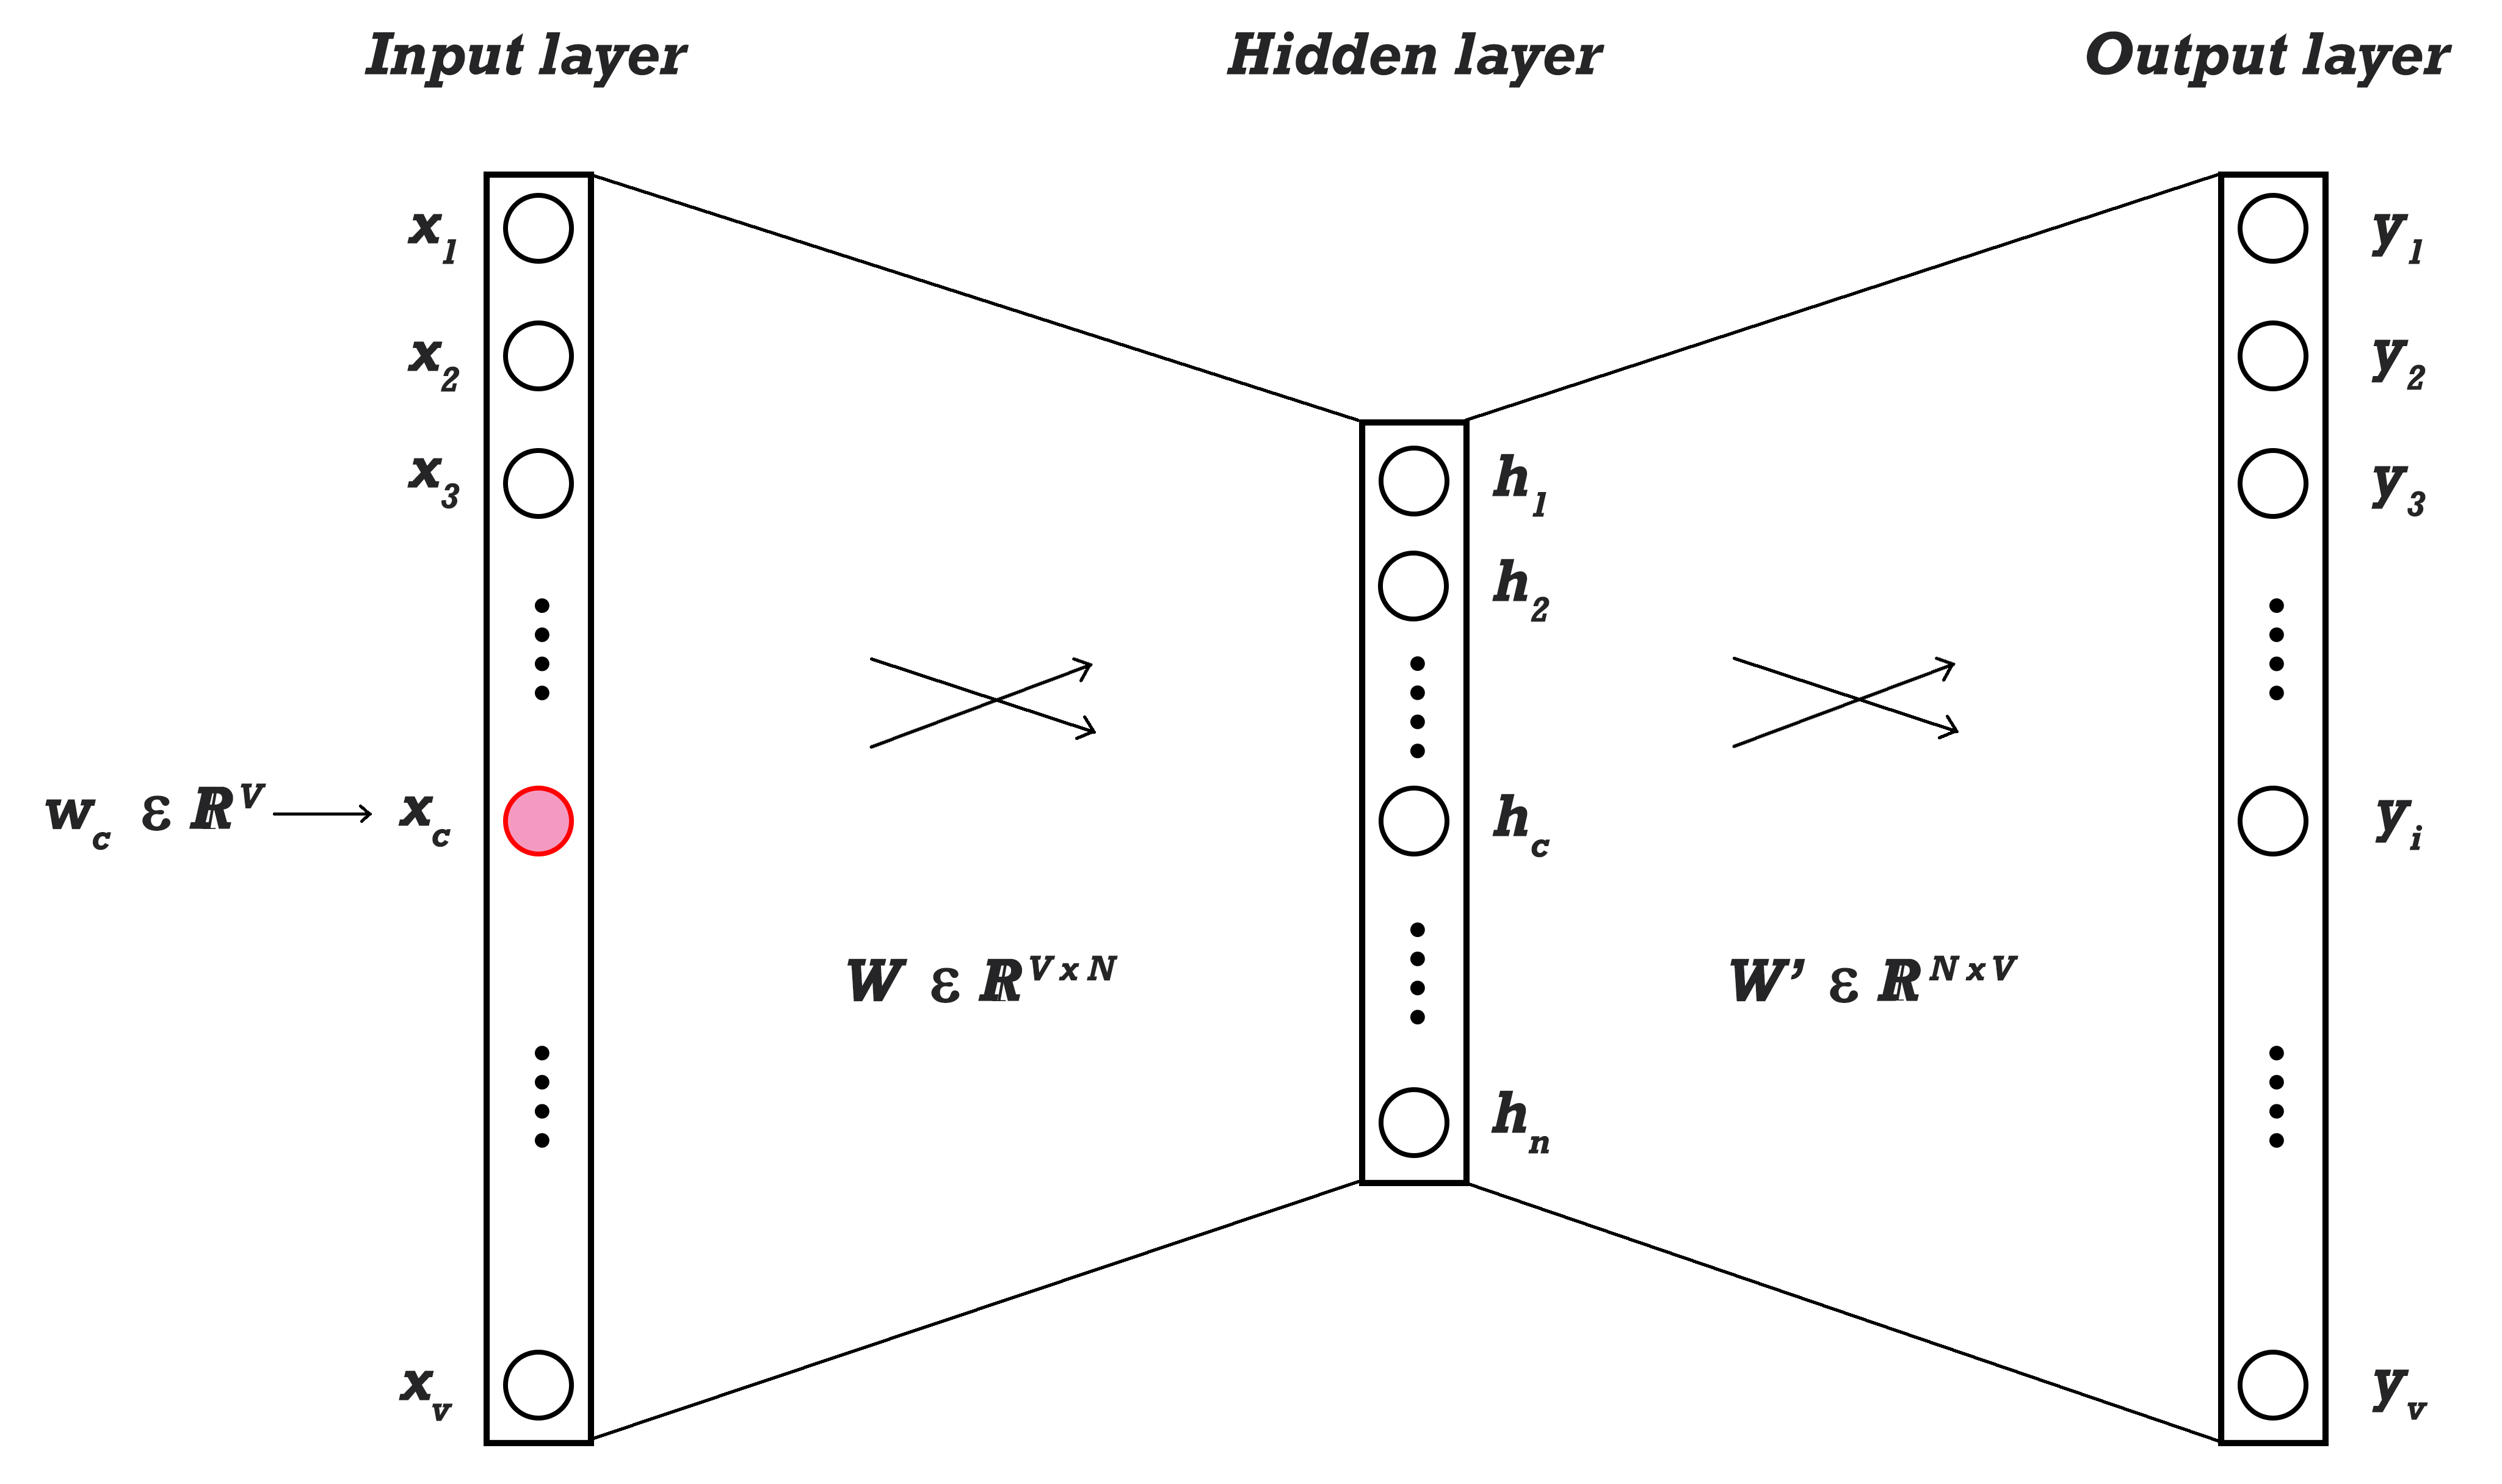
\includegraphics[width=0.8\linewidth,height=10cm,keepaspectratio]{cbow}
\caption[The CBOW model]{\textbf{The CBOW model: } In the CBOW model, the objective is to predict the target word from the words in the context (or neighbouring words). The context words are input to the model (in this case only one) using localist representation where only one vector element corresponding to input word is active ($x_{c}$, shown in red). The model outputs the probability for each word in vocabulary, which is maximized for actual target word during training. Adapted from [ref].}
\label{fig:cbow}
\end{figure}

\begin{figure}[hbtp]
\centering
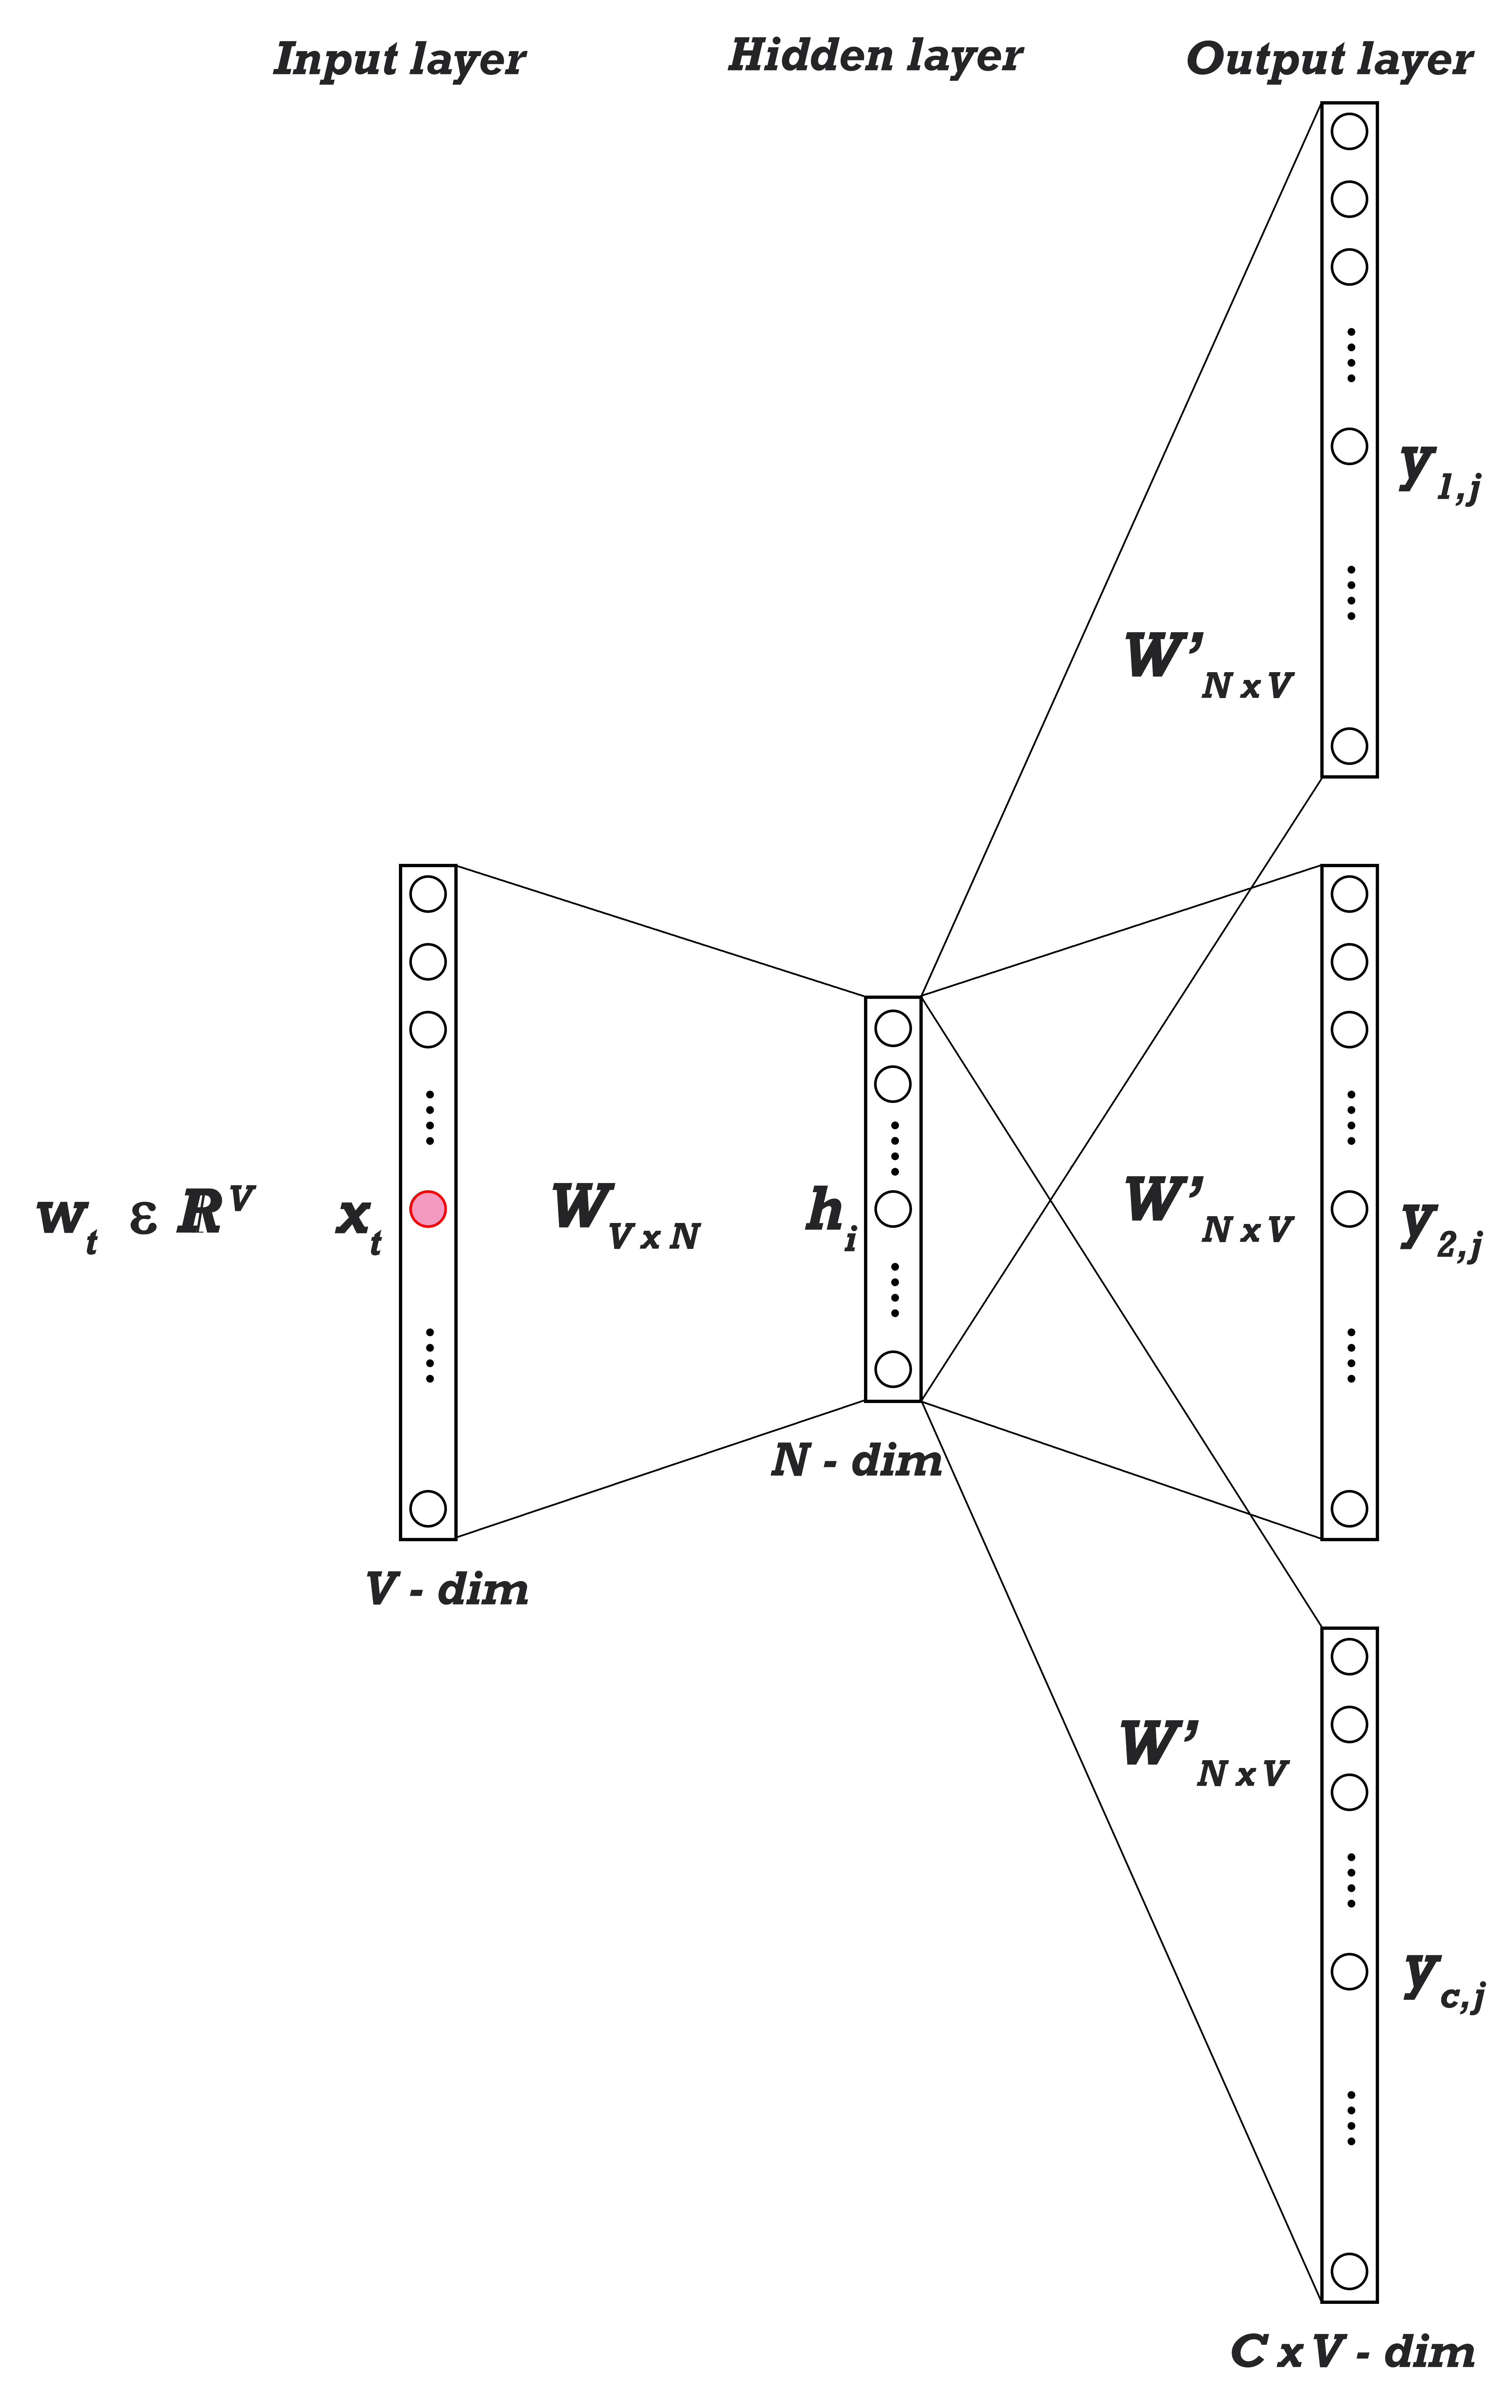
\includegraphics[width=1.8\linewidth,height=10cm,keepaspectratio]{sg}
\caption[The Skip-gram model]{\textbf{The skip-gram model: }In the skip model, the objective is reverse of CBOW. It predict the context words from the word. The target word is input to the model using localist representation where only one vector element corresponding to input word is active ($x_{t}$, shown in red). The model then maximizes the probaility of context words during training. Adapted from [ref].}
\label{fig:sg}
\end{figure}

\subsection{CBOW Model}

CBOW  model is a three layered neural model with the training objective to predict a target word (e.g. Peter) given some context words (John gave ball to …). Figure \ref{fig:cbow} shows the CBOW network architecture with a simplified case of one context word. The model is trained on the dataset having a vocabulary size $V$ in an unsupervised way to achieve the objective. The hidden layer is of size $N$, the dimensions of desired word embedding, and neurons in both the adjacent layer i.e. input and output layers,  are fully connected to hidden layer neurons. The input to the network is the context word $w_c {\in} \mathbb{R}^{V}$ and is represented using localist representation where only one unit $x_c$ at index c will be 1 out of V units $w_c=[{x_1,.....,x_V}]$ and all other units will be 0 \cite{w2v:parameter_learning}. The activation of hidden layer is then given by :

\begin{equation}\label{eqn:hidden_act}
	h = W^T . w_c= W_{(c,:)}=v_{c}
\end{equation}

where $W {\in} \mathbb{R}^{V{\times}N}$ is the weight matrix from input to hidden layer and $v_{c}$ is the vector embedding of the context word $w_c$. Eqn. \ref{eqn:hidden_act} basically copies the $c^{th}$ row of weight matrix $W$ on the hidden layer as hidden layer activation function is linear. 

A score $u {\in}\mathbb{R}^V$ is then calculated for all the target words in the vocabulary, which is essentially the compatibility of a word $w_i$ given the context word $w_c$.

\begin{equation}
\begin{split}
		 u &={W^{'}} ^ T . h \\
	   	   &= {W^{'}}^T. v_{c}	
\end{split}
\end{equation}

\begin{equation}
	u_i = {W^{'}_i}^T. v_{c}
\end{equation}

\noindent  where $u_i$ gives the score of $i^{th}$ word,$w_{i}$, for i = 1, 2...V. $W^{'}{\in} \mathbb{R}^{N{\times}V} $ is the weight matrix between hidden and output layer. ${W^{'}_i}$ is the $i^{th}$ column vector of matrix $W^{'}$.  
The computed scores are then converted to posterior probabilities by output neurons with softmax activation function. Thus aliasing ${W^{'}_i}$ as $v^{'}_{i}$ we get output probabilities as: 

\begin{equation}
\begin{split}	
y_i &= P(w_i | w_c) = \frac {\exp(u_i)} {\sum_{i' {\in} V} \exp (u_{i^{'}})}\\
	&= \frac {\exp({v^{'}_{i}}^T.v_{c})}{\sum_{i' {\in} V}\exp({v^{'}_{i^{'}}}^T.v_{c})}
\end{split}
\end{equation}
where $y_i$ is the probability of $i^{th}$ word given the context word.

The training objective is then achieved by maximizing the log likelihood of actual target word $(w_{t})$ given the context word ($w_{c}$). So the cost functions can be written as:

\begin{equation}
  \begin{split}
  	J_{ML} &= max \log P(w_t | w_c) \\
		   &= {v^{'}_{t}}^T.v_{c}- \text{ log} \sum_{i' {\in} V} {\exp({v^{'}_{i^{'}}}^T.v_{c})}
  \end{split}
\end{equation} 

In case of multiple context words is input to the network, the equation \ref{eqn:hidden_act} only change to:

\begin{equation}
h= \frac {1}{K} .(v_{c_1}+v_{c_2}+.......+v_{c_K}) 
\end{equation}	

where $k$ is the size of context window. This equation averages vector embeddings of all context words \cite{w2v:parameter_learning}.

\subsection{Skip-gram Model}

In the Skip-Gram model training objective is reversed from that of CBOW model. In other words, the objective is to learn the vector representation of the word that is good in predicting the context words \cite{w2v:mikolov_2013_distributed}. Thus for a given sequence of words $\{w_1,.....w_V\}$, the objective is to maximize the average log probability. 

\begin{equation}
\frac {1}{V}\sum_{t=1}^{V} \sum_{{-c \leq j \leq c},{j \neq 0}} {log\ P(w_{t+j}|w_t)}
\end{equation}

where c is the size of context window, $P(w_{t+c}|w_t)$ is the probability of context word $w_{t+j}$ for $-c \leq j \leq c$, given the target word $w_t$. This is measured using softmax function as:

\begin{equation} \label{eqn:sg_prob}
p(w_{t+j}|w_t)=\frac {\exp({{v^{'}_{t+j}}^{T}}.{v_t})}{\sum_{w {\in}V} \exp({{v^{'}_{w}}^{T}}.{v_t})}
\end{equation}

\noindent where ${v^{'}_{t+j}}$ and ${v_t}$ are the vector representation of word $w_{t+j}$ and $w_{t}$ respectively.

The objective function is thus optimized using stochastic gradient descent to learn the good word vectors. Calculating the full softmax is computationally expensive as it need to compute and normalize probability for every other word $w$ in the vocabulary V for a given input word ($w_{c}$ for CBOW or $w_{t}$ for skip-gram) at every training step. Thus negative sampling was proposed for learning the word embeddings\cite{w2v:mikolov_2013_distributed}.

\subsubsection{Skip-gram with negative sampling}

For learning word features full probabilistic models was not required. So in skip-gram negative sampling is used for approximation of word features. This technique treats feature learning as a binary classification (logistics regression) problems \cite{w2v:mikolov_2013_distributed, w2v:tensor_flow}. The model is thus trained to distinguish the target word from $k$ imaginary noise words $w_{noise}$, in the same context. Thus the log probability $p(w_{t+j}|w_t)$ in equation \ref{eqn:sg_prob} is now approximated by:

\begin{equation}
p(w_{t+j}|w_t)=log\ \sigma({{v^{'}_{t+j}}^{T}}.{v_t})\ +\  \sum_{w_{noise}{\in}N_{k}} \log\ \sigma({{v^{'}_{noise}}^T}.v_{t})
\end{equation}

\noindent where $\sigma(x)=1/(1+\exp(-x))$, and $N_k$ is the set of $k$ noise word compared to corresponding context word $w_{t+j}$ for $-c \leq j \leq c$. 

\subsection{Properties of Word2Vec embeddings}

Although the word2vec model is simple in architecture and easy to train, it produces word vector embedding which surprisingly encodes several linguistic regularities and patterns \cite{w2v:language_similarities, w2v:mikolov_2013_distributed}. More importantly it is astonishing because the network was not explicitly trained for these linguistic properties (see fig. \ref{fig:sem_rel} and \ref{fig:w2v_translation}). The distributed word embeddings encodes semantic and syntactic properties of the words as a constant vector offset between a pair of words sharing a specific relationship\cite{w2v:mikolov_2013_distributed}. For example, the word embeddings $"King - Queen \approx man - woman"$, $"apples - apple \approx cars - car"$, $"walking - walked \approx swimming - swam"$.

\begin{figure}[hbtp]
\centering
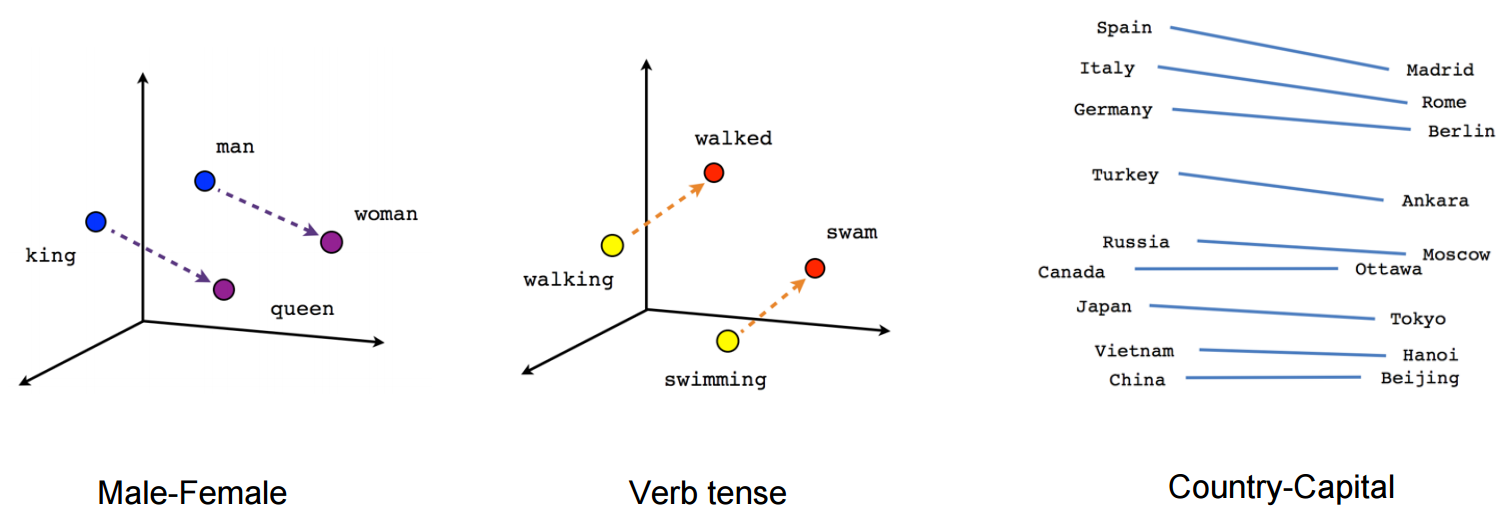
\includegraphics[width=0.8\linewidth]{linear-relationships}
\caption[Word2vec semantic regularities]{\textbf{Word2vec semantic regularities.}} 
\label{fig:sem_rel}
\end{figure}

\begin{figure}[hbtp]
\centering
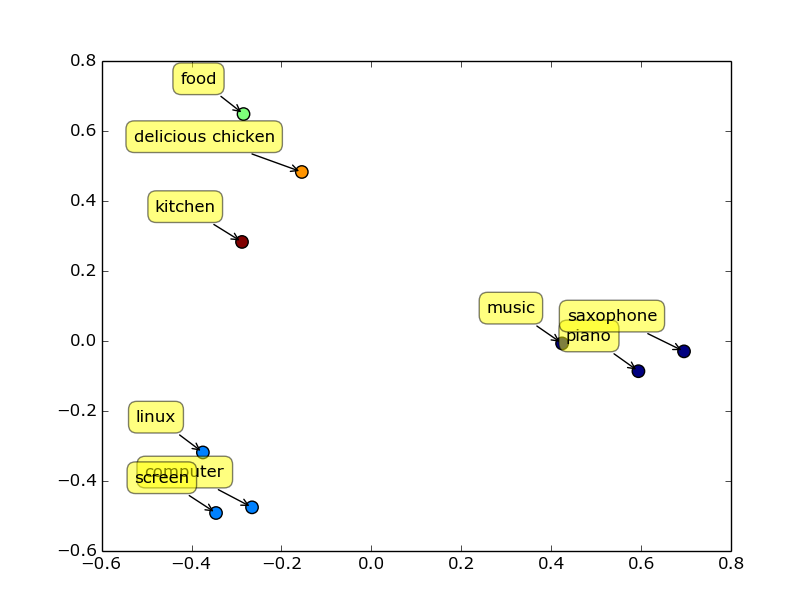
\includegraphics[width=0.8\linewidth]{word2vec_clustering}
\caption [Word2Vec word clustering]{\textbf{Word Clustering with word2vec word embedding:} The figure shows the word clustering property obtained by projecting the word vectors on two dimesional space using PCA. The words vector taken from pretrained word2vec Google News corpus\footnotemark }
\label{fig:w2v_clustering}
\end{figure}

\footnote{https://drive.google.com/file/d/0B7XkCwpI5KDYNlNUTTlSS21pQmM/edit}

\begin{figure}[hbtp]
\centering
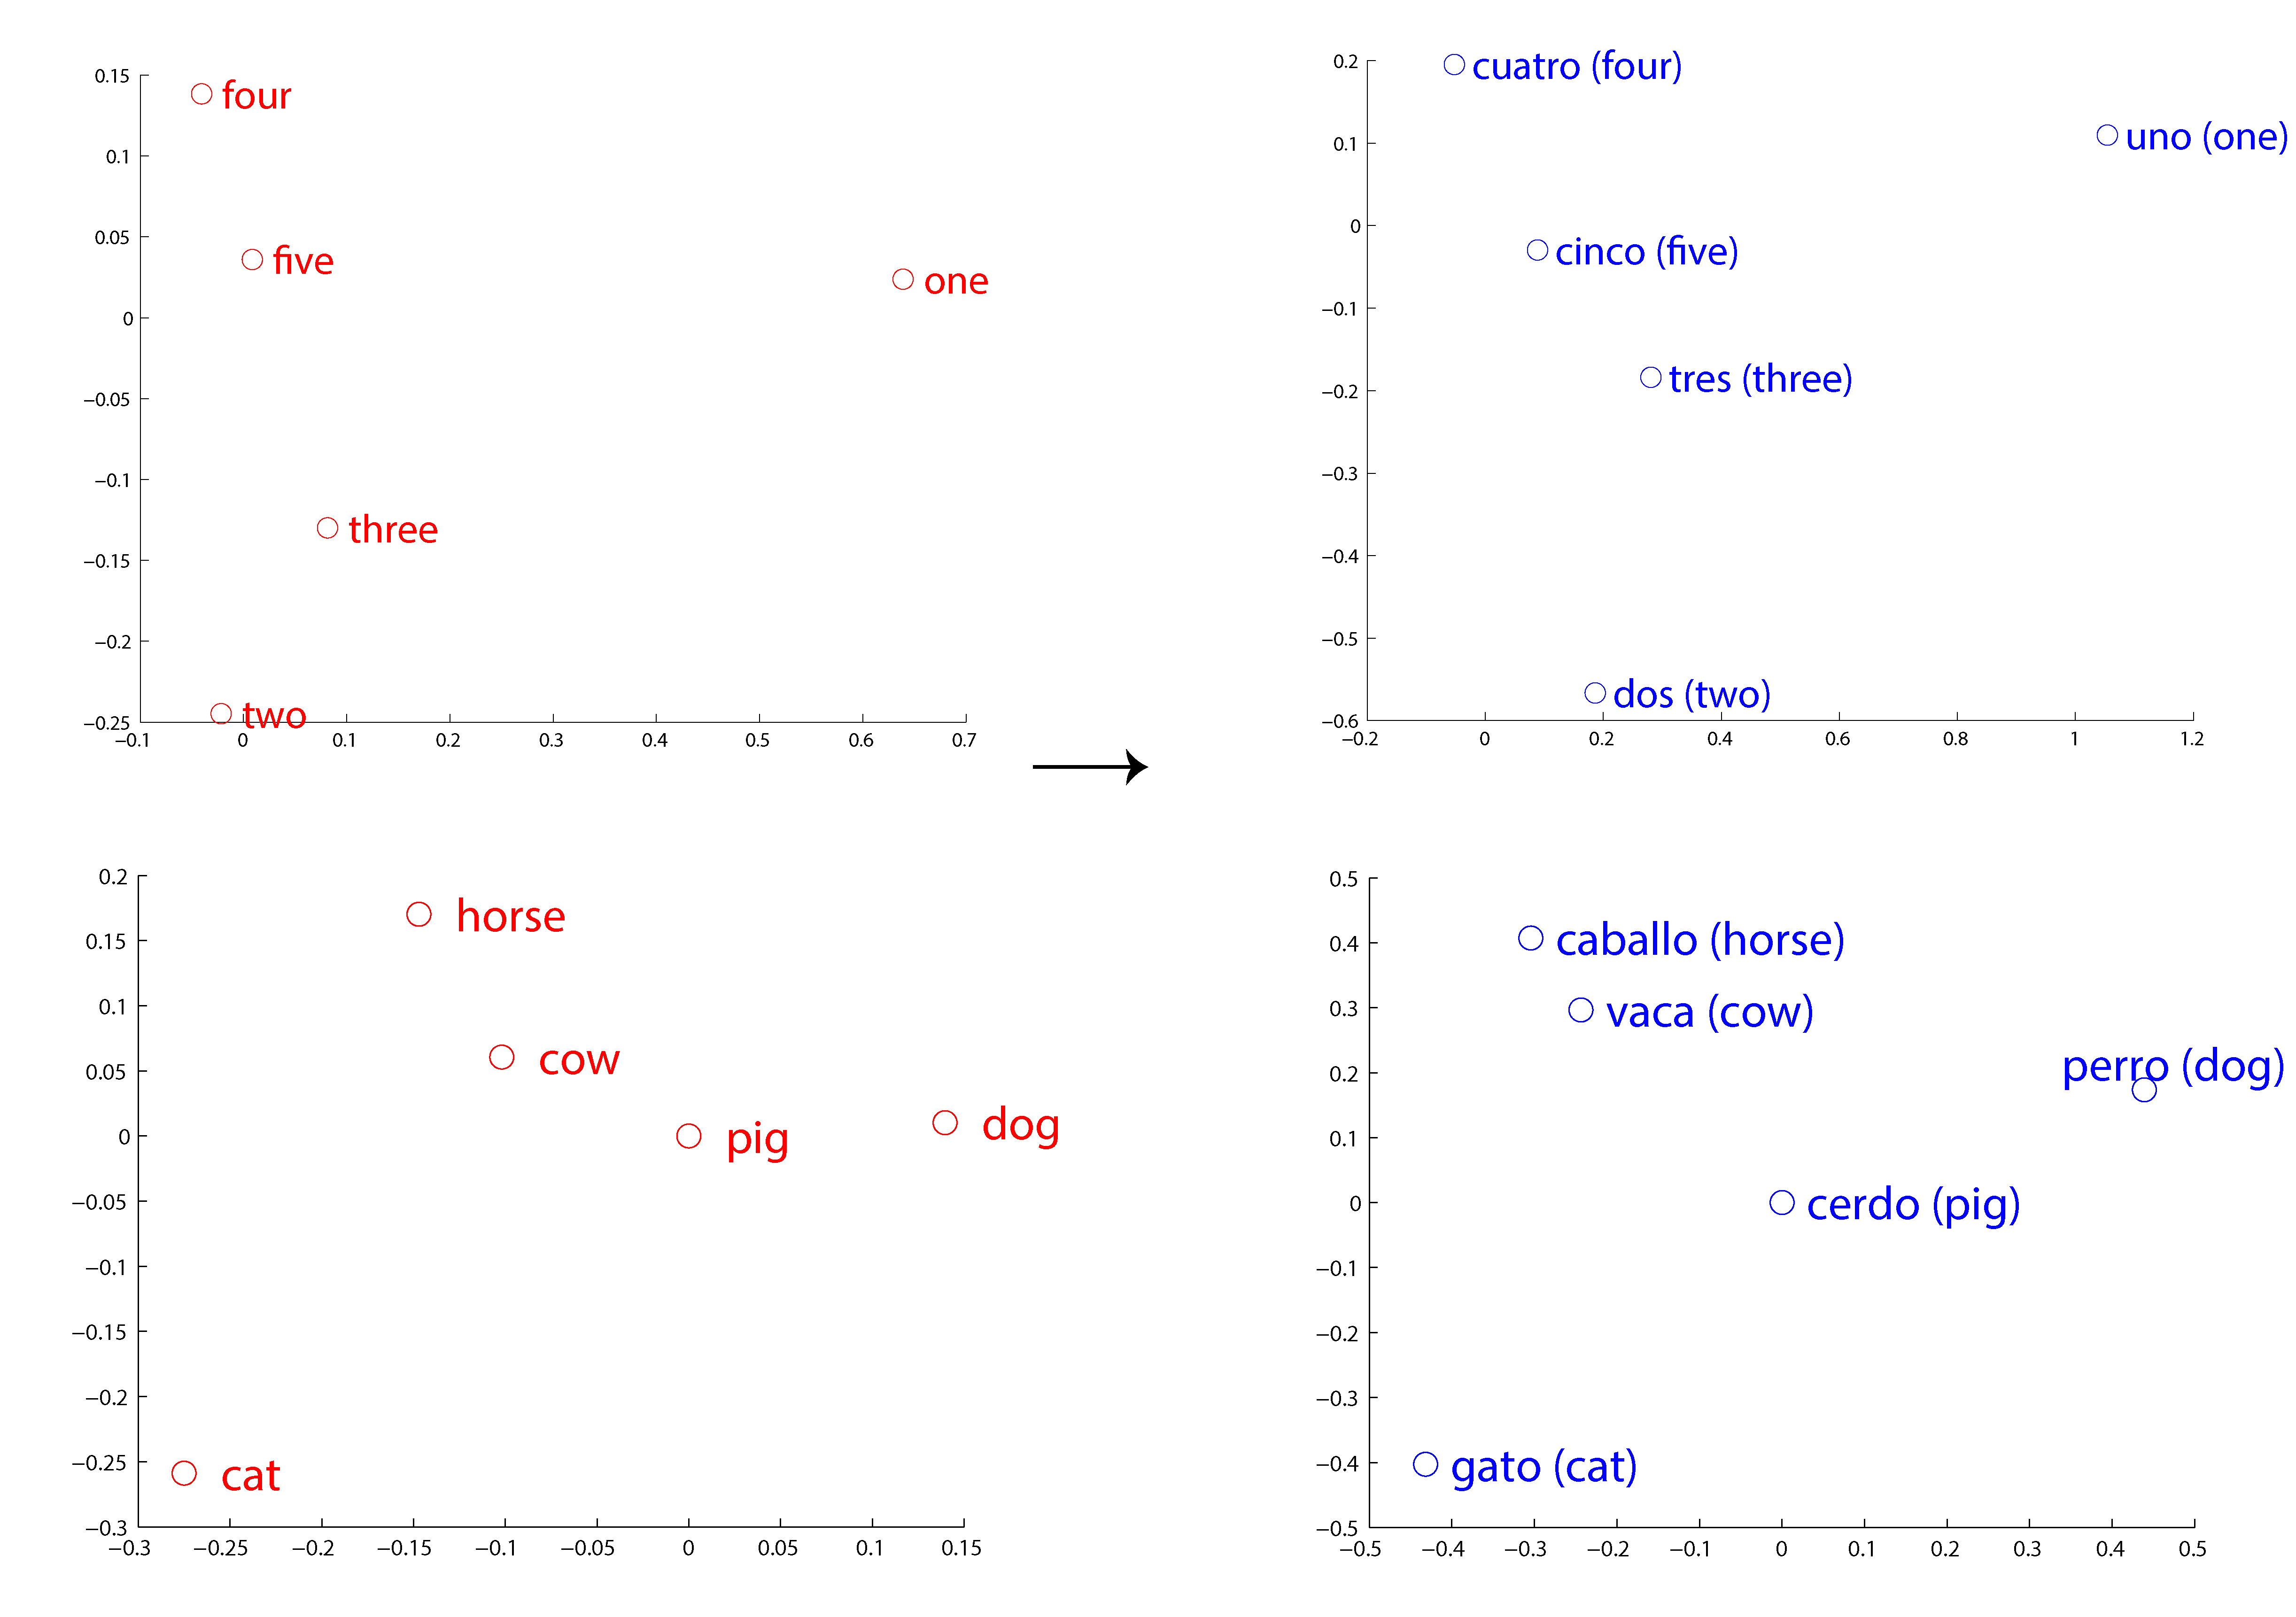
\includegraphics[width=0.8\linewidth,height=10cm,keepaspectratio]{word2vec_translation}
\caption[Word2Vec language translation property]{\textbf{Word2Vec language translation property.}}
\label{fig:w2v_translation}
\end{figure}

The another interesting property is that the the semantically related words are placed close to each other in word vector space, thus forming clusters of semantically related words. It was also observed the word embeddings of similar words in different languages have the same geometrical arrangement in embedding space of respective language. Thus it is also possible to learn linear mapping between different embedding space by vector rotation and scaling \cite{w2v:language_similarities}. Several other regularities can also be captured by performing basic linear operation on word-embeddings \cite{w2v:mikolov_2013_distributed}. 

\section{Echo State Network (ESN)}

Echo State Network (ESN) is a network with a new viewpoint on Recurrent Neural Network (RNN). It is a discrete time continuous state recurrent neural network introduced by Herbert Jaeger \cite{esn:jaeger:2001} and is believed to closely resemble the learning mechanism in biological brains. ESN is found to be computationally simple and inexpensive to process the temporal or sequential data. The main idea of ESN is to operate the random, large, fixed RNN with the input signal and the non-linear response generated by each neuron of the RNN is collectively combined with the desired output signal using regression to learn the output weights \cite{esn:jaeger_tutorial, esn:jaeger:2001,esn:scholarpedia:2007}.

\subsection{ESN Architecture}

ESN is surprisingly efficient variant for RNN training (see fig. \ref{fig:esn_arch}). In the standard RNN all the weights are required to be tuned even-though it was shown that RNN works well enough even without full adaptation of weights. The classical ESN mainly contains three layers, input layer, the hidden layer (also known as reservoir) and the readout layer. The input layer is fully connected to the hidden layer and both the hidden layer and the input layer is connected to the output layer. The output layer is fully connected back to the hidden layer. However the connection from input to output layer and output layer to hidden layer is optional and depends on the task.

The weights from input to reservoir (i.e. $W^{in}$) and from reservoir to reservoir (i.e. $W^{res}$), are sparsely and randomly initialized and more crucially remains untrained during training. The non-zero element in sparse input weight matrix $W^{in}$ and reservoir weight matrix $W^{res}$ are generated from uniform or normal distribution. The weights from the reservoir to output layer (i.e. $W^{out}$) are the only weights learned during supervised training \cite{esn:jaeger:2001, esn:practical_guide}. For ESN approach to work the reservoir should possess the Echo State Property: if a long input sequence is given to the reservoir the reservoir will end up in the same state irrespective of the initial reservoir state. In other word the reservoir states 'echoes' the input sequence and the effect of previous reservoir state and the previous input on the future reservoir states should vanish gradually \cite{esn:practical_guide, esn:jaeger_tutorial}. 

\begin{figure}[hbtp]
\centering
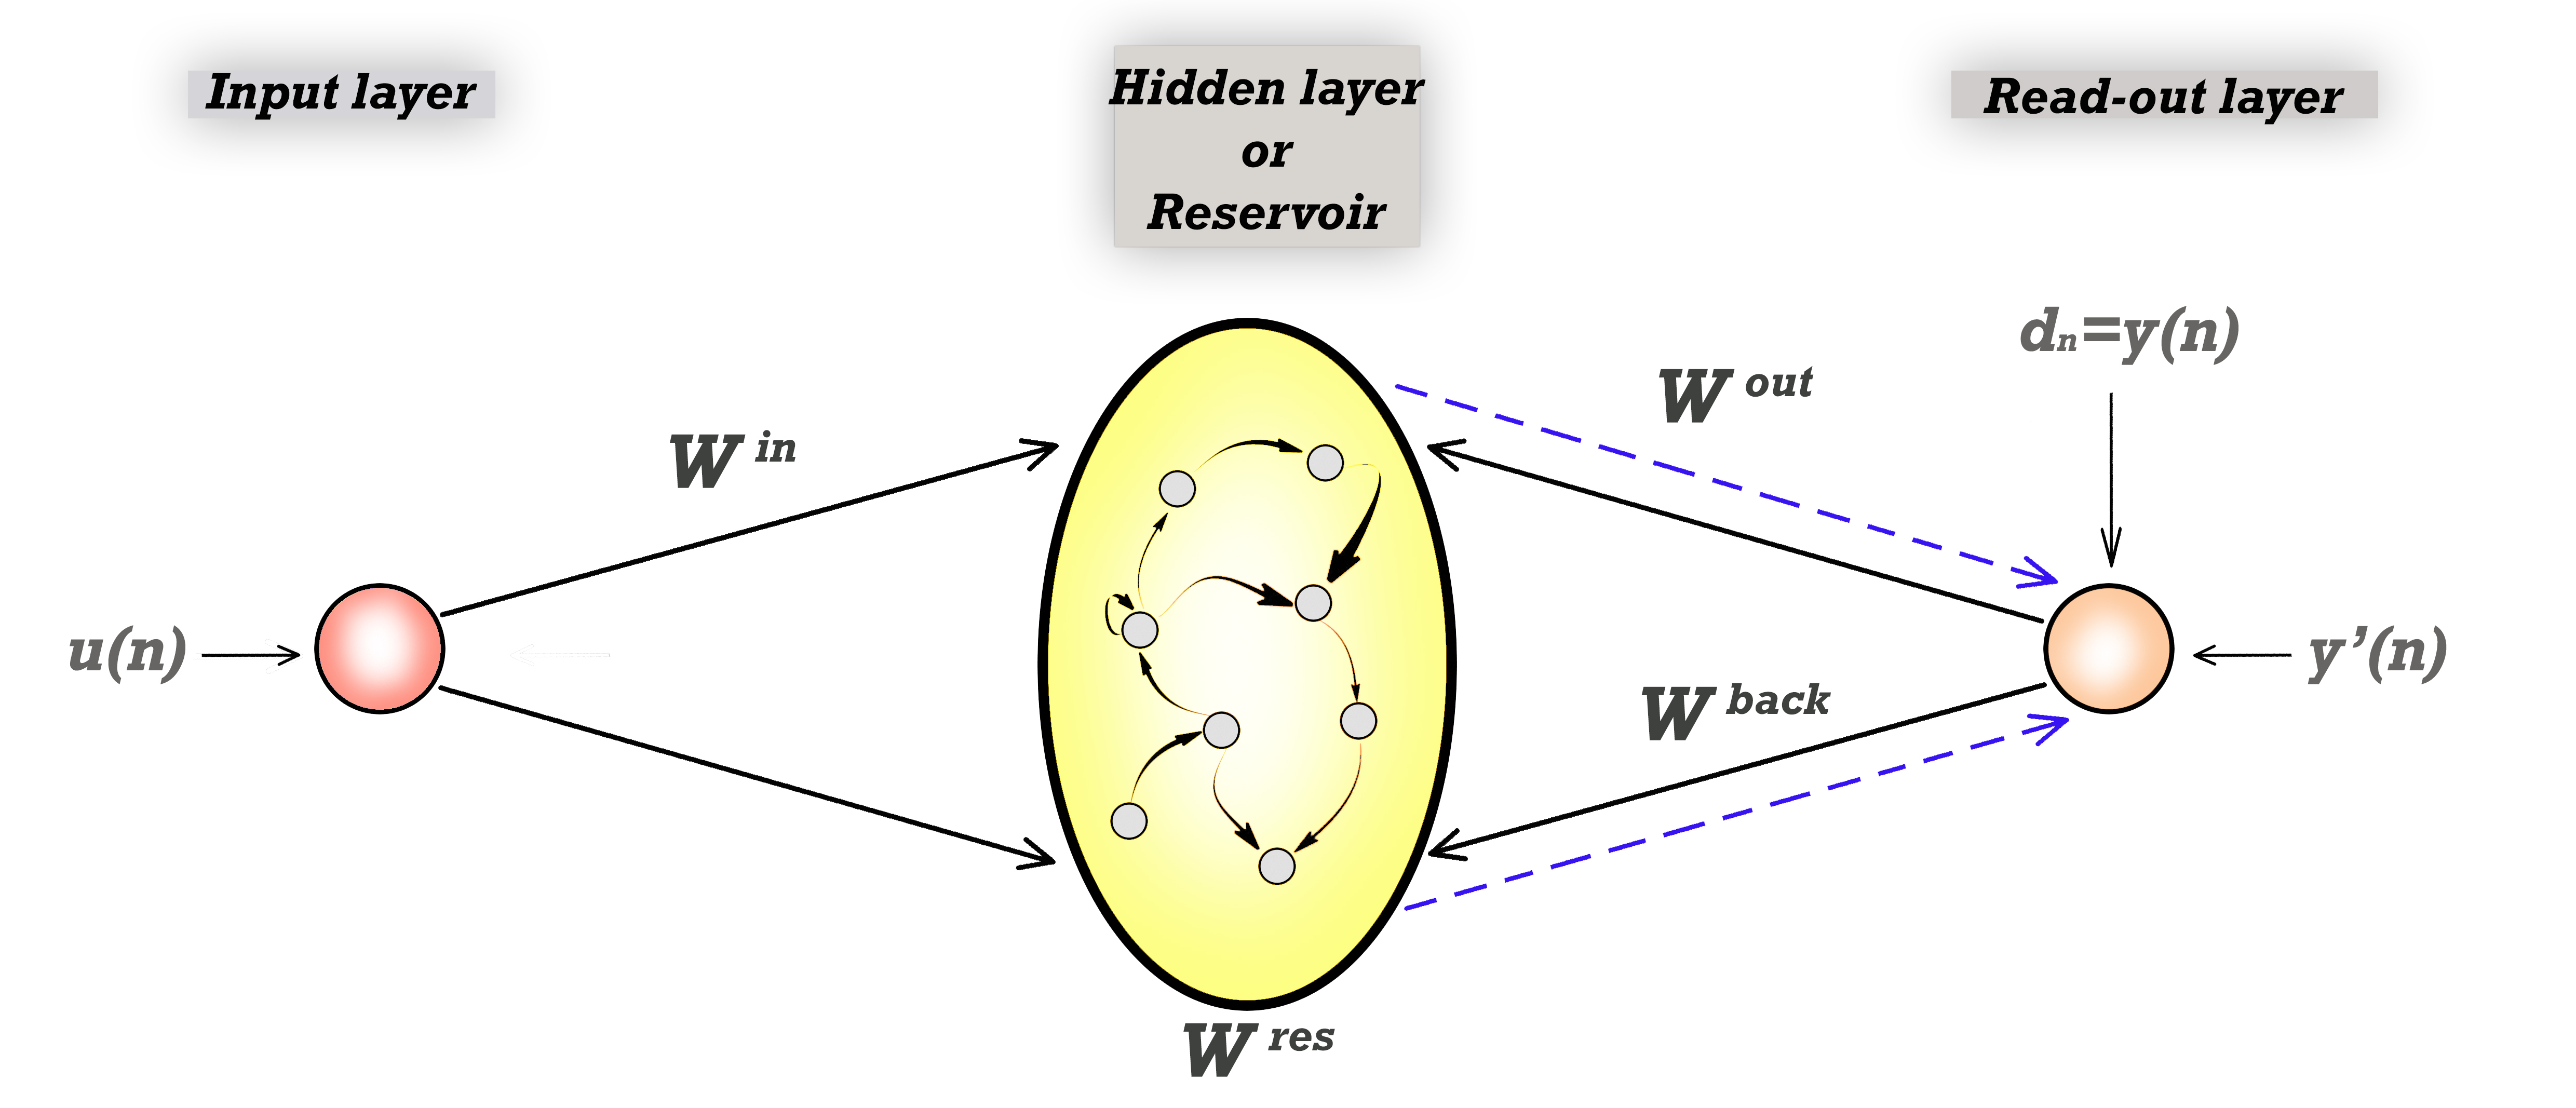
\includegraphics[width=0.8\linewidth]{esn_architecture}
\caption[Architecture of classical ESN]{\textbf{Architecture of classical ESN:} The reservoir is the recurrent neural network with $N_{x}$ units and initialized with random connection. The reservoir is provided input $u(n)$ to the input layer and teacher layer $y(n)$ are pushed output neurons  respectively during training. The input to reservoir weights ($W^{in}$), output neurons to reservoir ($W^{back}$, optional and depends on task) and reservoir to reservoir weight ($W^{res}$) from are also randomly initialized and stays static during learning. The output weight from reservoir to output unit are the only weights learned by the network during training. Adapted from \cite{esn:practical_guide}}
\label{fig:esn_arch}
\end{figure}

To ensure the echo state property in ESN, firstly, the reservoir weights matrix $W^{res}$ and the input weights matrix $W^{in}$ are often generated sparsely (i.e. most of the elements in these matrices will be zero) and randomly from a normal or uniform distribution \cite{esn:practical_guide}. The input weight matrix is however a bit more denser than the reservoir weight matrix. The sparsely generated random reservoir weights matrix $W^{res}$ is often scaled such that its spectral radius $\rho(W^{res})$ i.e. largest absolute eigenvalue, is less than one. To scale the randomly generated $W^{res}$ matrix, it is first divided by its spectral radius and then multiplied with desired spectral radius \cite{esn:jaeger_tutorial}.

\begin{equation}\label{eqn:res_scaling}
W_{new}^{{res}}=\gamma \frac{W^{res}}{\rho(W^{res})}
\end{equation}

where $W_{_{new}}^{{res}}$ is the scaled reservoir weight matrix, $0 < \gamma < 1$ is the desired spectral radius and $\rho(W^{res})$ is the spectral radius of randomly generated reservoir Matrix $W^{res}$.

It is also argued that the $\rho(W^{res}) < 1 $ is not a necessary condition for ESN to have the echo state property and can be achieved even when $\rho(W^{res}) > 1$ \cite{esn:jaeger:2001, esn:practical_guide, esn:jaeger_tutorial}. Intuitively, the spectral radius is a crude measure of the amount of memory the reservoir can hold, the small values meaning a short memory, and the large values a longer memory, up to the point of over-amplification when the echo state property no longer holds. The input weights are also scaled to regulate the non-linearity in reservoir activations. A very high input scaling let the reservoir to behave in highly non-linear manner (because of tanh activation function) whereas a very small input scaling is used wherever linearity is required in a task \cite{esn:practical_guide}.

\subsection{Training ESN}\label{ssec:esn_training}

ESNs are mostly applied supervised machine-learning tasks where temporal or sequentail aspect of the data is to be modeled. Before training, the reservoir of size $N_{x}$, generally containing leaky-integrated discrete-time continuous-value neurons with \textit{tanh} activation function is generated. The reservoir of any computationally affordable size can be used. The bigger the reservoir size, the more the input signal gets non-linearly expanded and easier it will be to find linear combination with the desired output signal \cite{esn:practical_guide, esn:jaeger_tutorial}. With the big reservoir size comes the risk of over-fitting. Thus, It is also important to use proper regularization methods to avoid over-fitting. The reservoir weight $W^{res}$, input weights $W^{in}$ and $W^{back}$ are then randomly initialized.

The training objective of ESN approach is to learn a model which outputs $\textit{y'}$, such that it is as close as possible to the target output \textit{y} by mining the error measure $E(y',y)$ and also generalize well on the data not used for training. Root Mean Square Error is typically chosed as erorr measure E. Thus during training, the given training input signal $\textit{u(n)} \in \mathbb{R}^{N_u}$ and the corresponding teacher signal $\textit{y(n)} \in \mathbb{R}^{N_y}$  is input to the reservoir at every time-step 'n'. Here n = 1,2...,T is the discrete time step for sequence of length T. The reservoir then generate a sequence $\textit{x(n)}$ of $N_{x}$-dimensional reservoir states which is non-linear high dimensional expansion of the input signal $\textit{u(n)}$ \cite{esn:jaeger_tutorial}. The reservoir activation and reservoir state update is computed using following recursive equations:

\begin{equation} \label{eqn:res_update}
x'(n) =\textit {tanh } ( W^{res}x(n-1) + W^{in}.u(n) + W^{back}.y(n-1))
\end{equation}
\begin{equation} \label{eqn:res_state}
x(n) =\textit (1-\alpha) x(n-1) + \alpha x'(n)
\end{equation}

where $\textit{ x(n)}$ is the vector of reservoir neuron's activations and $\textit{ x'(n)}$ is its update at time step $\textit{n}$. \textit{tanh} is reservoir neuron activation function. $ W^{in} \in \mathbb{R}^{{N_x} \times{N_u}}$ and $ W^{res} \in \mathbb{R}^{{N_x} \times{N_x}} $ are input weights and reservoir weights matrices respectively. $ W^{back} \in \mathbb{R}^{{N_x} \times{N_y}} $ is the optional output to reservoir matrix \footnote{this weight matrix is not used in our model implementation}. $\alpha \in (0,1]$ is leaking rate of neurons.  

The leaking rate, $\alpha$, regulates the speed of reservoir update dynamics in discrete time. Smaller value of also induces slow reservoir dynamics thus ensuring the long short-term memory in ESN \cite{esn:practical_guide, esn:optimization_leaky_neurons}. The reservoir activation states are accumulated at every time step for regression with the teacher output. The linear readout weights are then learned using equations:

\begin{equation}\label{eqn:esn_output}
y'(n) = \textit W^{out}x(n)
\end{equation}

where $y'(n) \in \mathbb{R}^{N_y}$ is output of the network and $W^{out} \in \mathbb{R}^{{N_y} \times {N_x}}$ is the output weight matrix.

Writing the equation \ref{eqn:esn_output} in matrix form, the output weights $W^{out}$ are then learned using the following equation:
 
\begin{equation}
Y=W^{out}X
\end{equation}
\begin{equation}
W^{out}=YX^{T}(XX^{T}+{\beta}I)^{-1}
\end{equation}

where $\beta$ is the regularization coefficient parameter of ridge regression and \textit{I} is the Identity matrix. 

Training procedure of ESN, have only few global parameters which are to be optimized: reservoir size $ N_{x} $, spectral radius of $W^{res}$, input scaling of $W^{in}$, leak rate $\alpha$ and the ridge parameter $\beta$. All these parameters can only be optimized by trial and error method and depends heavily on the task under consideration. Usually a grid search is applied to explore the best parameter combination.   

\cleardoublepage

\chapter{Related Work and Open Issues}\label{issues}

Humans have a remarkable ability of perceiving and comprehending one or more languages. But how do they know what does a sequence of symbols means? In other words, how do they link a sequence of words to its meaning? With this research question, Hinaut et al. \cite{xavier:2013:RT} proposed a neuro-inspired model, $\theta RARes$, to process the sentence across time without having to know the semantics of the words. The model used reservoir computing approach namely echo state network and implemented on robotics architecture \cite{tra:xavier_hri} for the thematic role assignment task. This was the first time when echo state network was used for thematic role assignment task. The experiments done for TRA showed the results toward modeling of language acquisition in brain \cite{tra:xavier_wermter:2014,xavier:2013:RT}. The model was based on the cue competition hypothesis of Bates et al. \cite{tra:bates:1982} which states that closed class words (e.g. prepositions, articles, determiners, pronouns etc.), the order of words and prosody in a sentence encodes the grammatical structure. 

\section{Overview of $\theta RARes$ Model}\label{sec:xavier_model}

$\theta RARes$ Model is basically an echo state network, used to learn and predict thematic roles of the input sentences. The model is based on the notion of grammatical construction. The grammatical construction of a sentence is defined as the mapping of the surface form (word order) of the sentence to its meaning \cite{gc:goldberg:1995}.Figure \ref{fig:tra_gc} represents the characterization of thematic role assignment in grammatical construction form. The model does not take in input the raw sentences but instead use the abstract form of the sentences. The abstraction marks each word of a sentence into two kinds of symbols: Function Words and Semantic Words. Semantic words are the open class words like nouns, verbs, adjectives, adverbs etc. whereas Function words are closed class words like determiners, prepositions, articles, pronouns and verb inflections like -ed,-ing or -s etc.. Thus before giving a sentence as an input to ESN, all the semantic words are replaced with a unique token 'SW' and pushed to FIFO memory stack(see fig. \ref{fig:xavier_model}). The functional words were left unchanged unchanged (see table \ref{tab:localist_representation}).

\begin{figure}[hbtp]
\centering
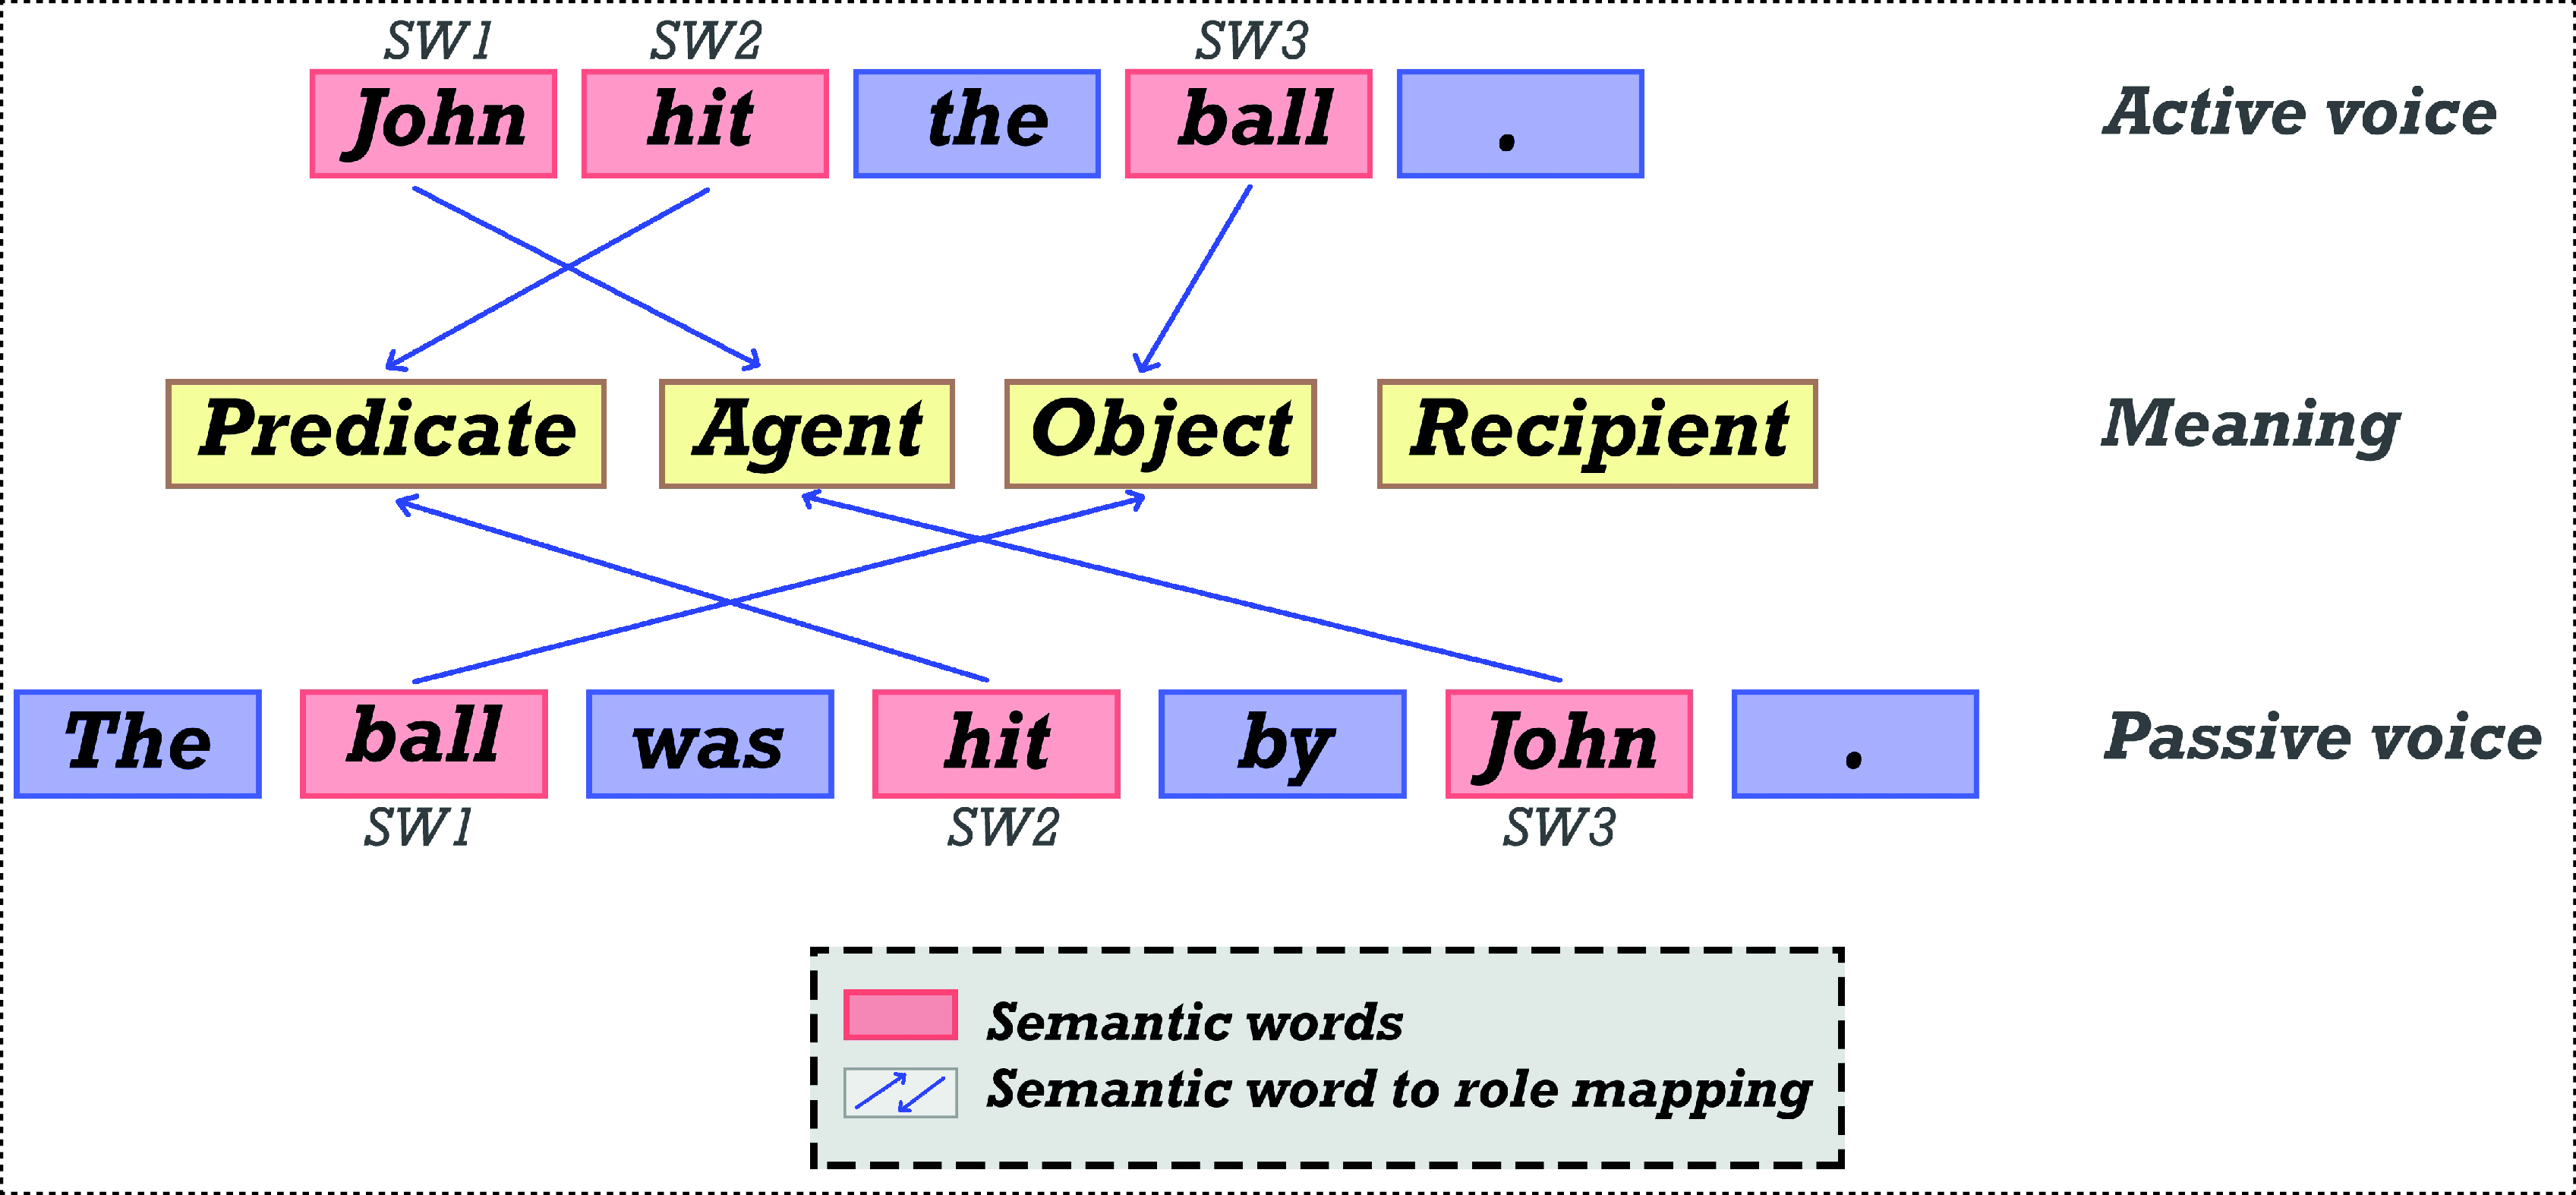
\includegraphics[width=0.8\linewidth,height=3.5cm, keepaspectratio]{grammatical_construction}
\caption[Word2vec semantic regularities]{\textbf{Word2vec semantic regularities.}} 
\label{fig:tra_gc}
\end{figure}

\begin{table}[hbtp]
\centering
\caption[Localist vector representation of sentence]{Transformation of a sentence by replacing semantic words with 'SW' token and localist vector representation of words used as an input for a sentence.}
\begin{tabular}{|c|c|c|c|c|c|c|c|}
\hline
\textbf{Original words} & \textbf{Transformed words}  & \multicolumn{6}{c|}{\textbf{Localist vectors}} \\ \hline
put		&	SW     & 0   & 1  & 0  & 1  & 0  & 1  \\ \hline
the		&	the    & 0   & 0  & 1  & 0  & 0  & 0  \\ \hline
ball	&	SW     & 0   & 1  & 0  & 1  & 0  & 1  \\ \hline
on		&	on     & 0   & 0  & 0  & 0  & 1  & 0  \\ \hline
the		&	the    & 0   & 0  & 1  & 0  & 0  & 0  \\ \hline
box		&	SW     & 0   & 1  & 0  & 1  & 0  & 1  \\ \hline
\end{tabular}
\label{tab:localist_representation}
\end{table}

\begin{figure}[hbtp]
\centering
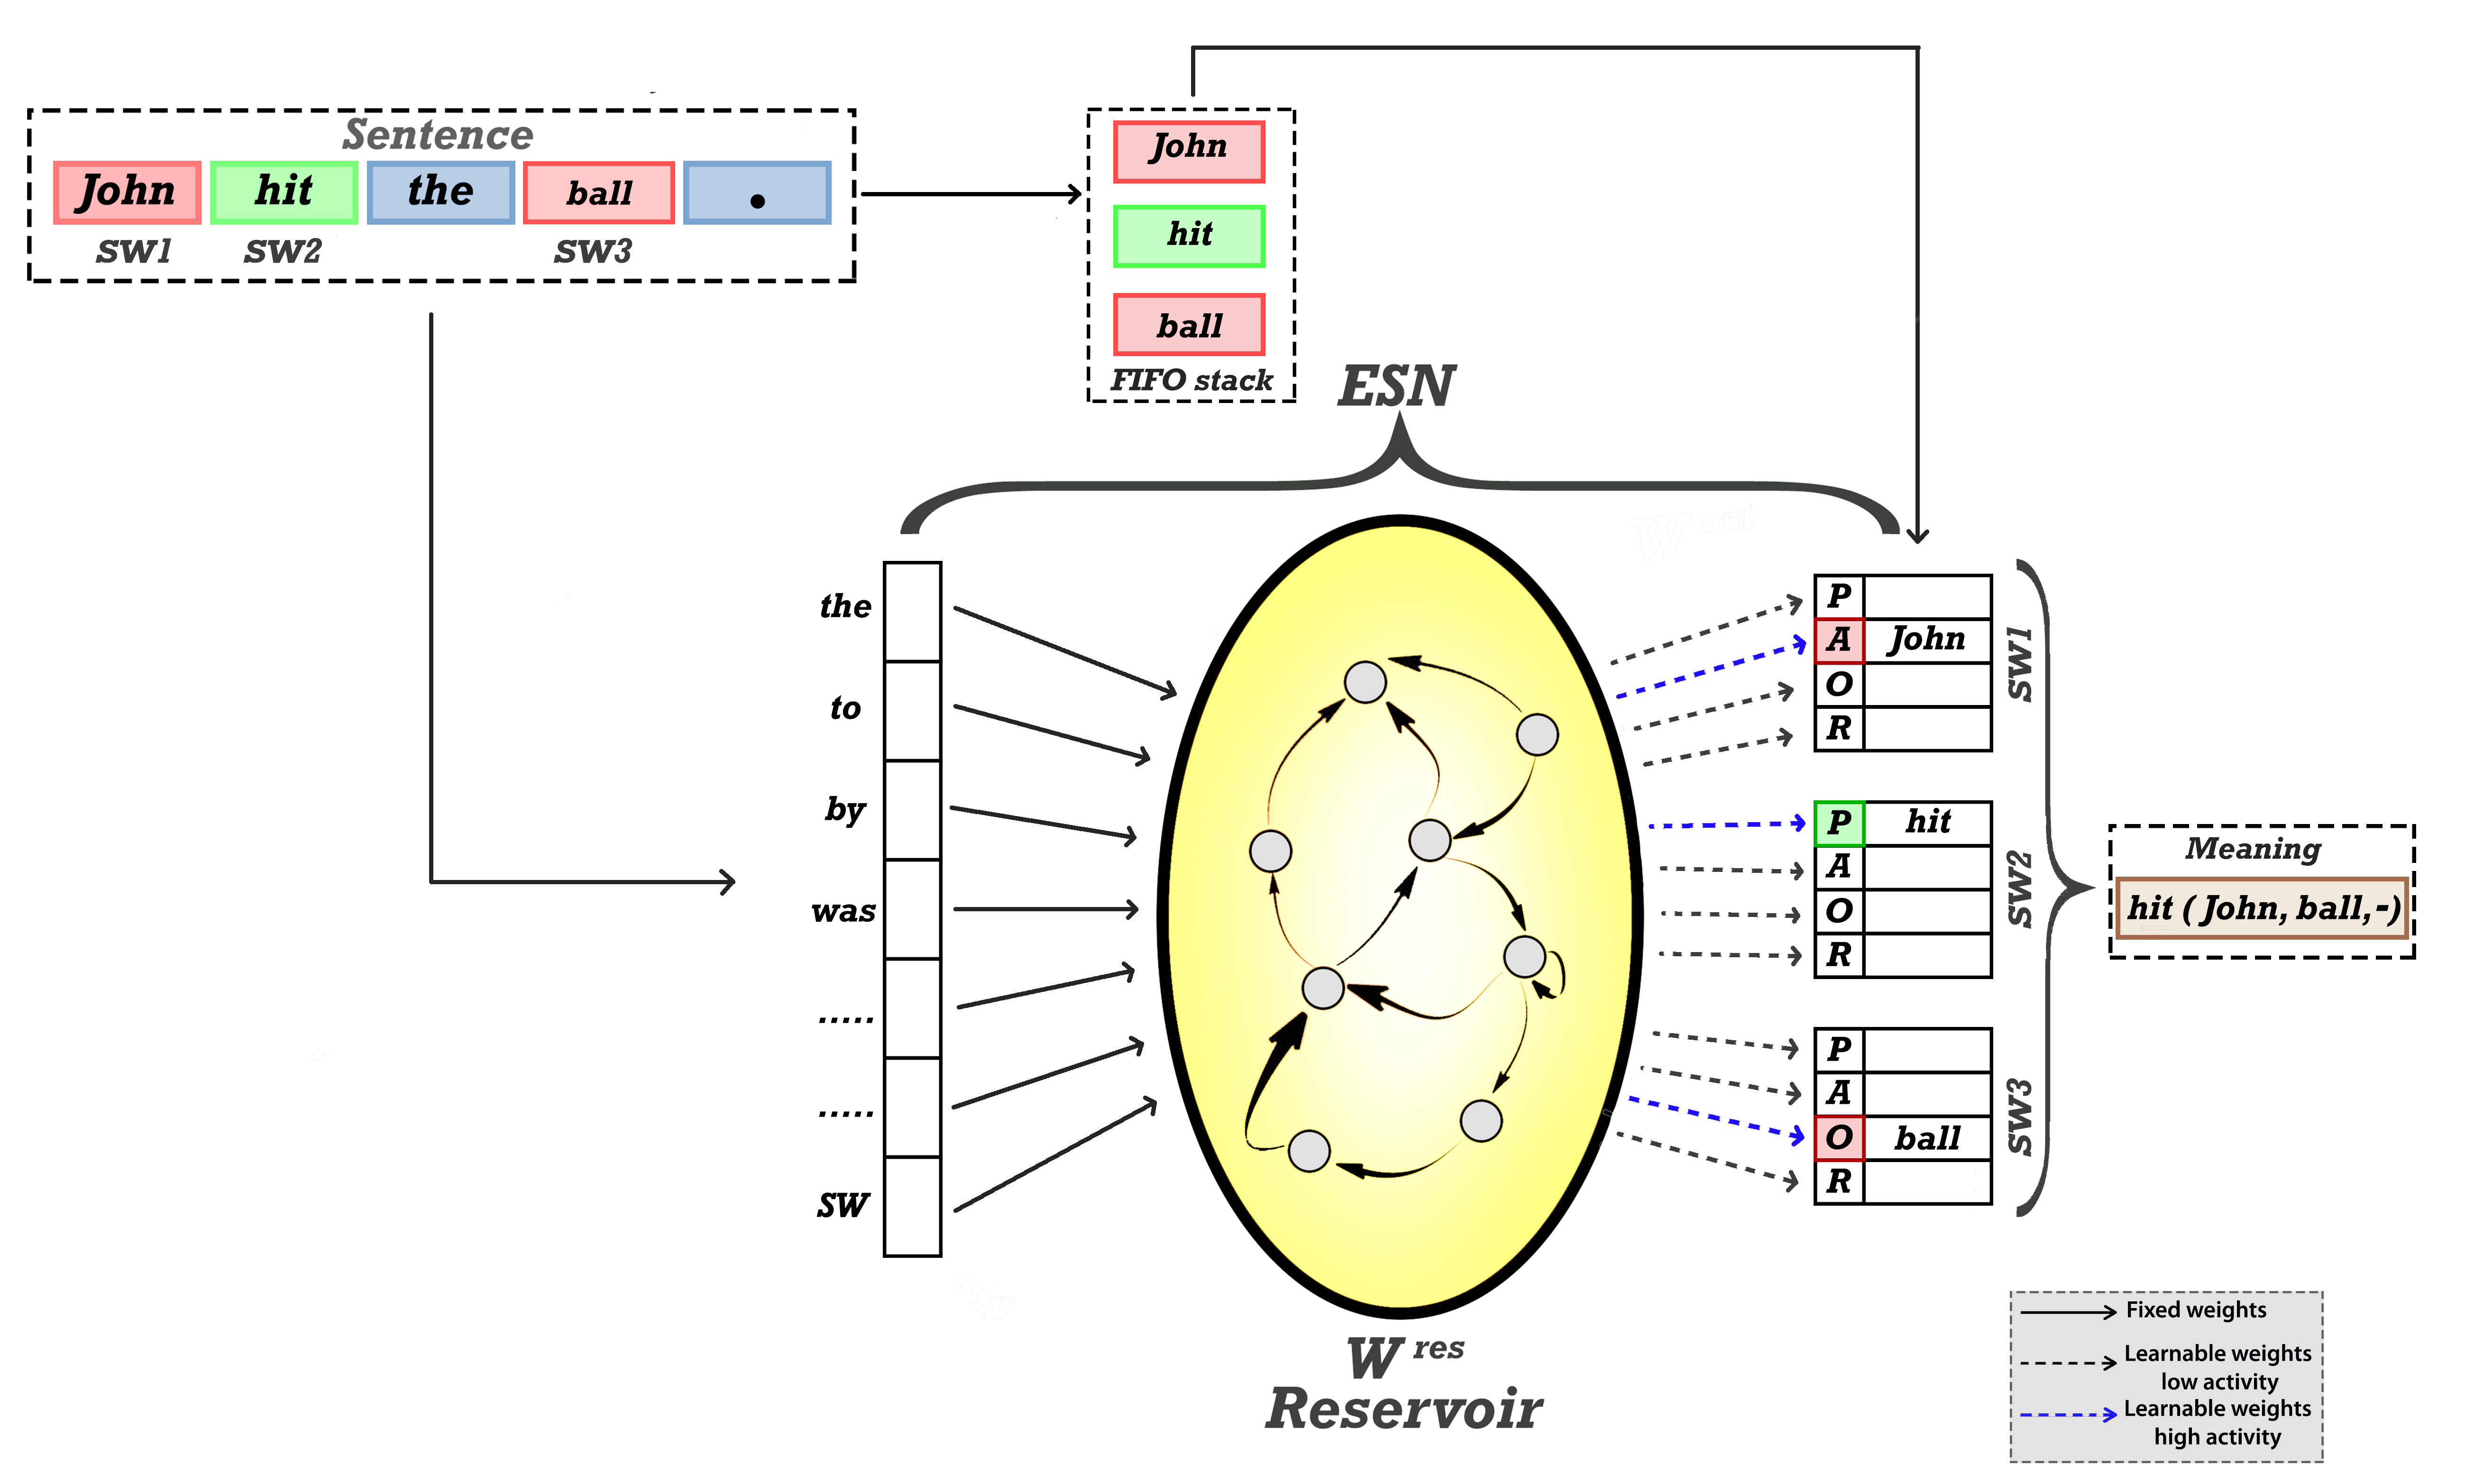
\includegraphics[width=0.8\linewidth]{xavier_model}
\caption[Word2vec semantic regularities]{\textbf{Word2vec semantic regularities.}} 
\label{fig:xavier_model}
\end{figure}

Thus for training the transformed sentences were presented to the model sequentially, word-by-word. Considering each word as a discrete atomic symbol, the words were encoded using localist vector representation, where all elements except the current input are zeros (see table \ref{tab:localist_representation}). Figure \ref{fig:xavier_model} shows the functional organization of the model. The localist word vectors are projected on the input layer of ESN and coded meaning of the input sentence is teacher-forced on the output layer of ESN. The model learns the thematic roles of all semantic words by learning reservoir to readout weights of ESN. During the testing, the model predicts the coded meaning of the test sentence. The output activation is decoded to its meaning by thresholding the activation at last time step. For each SW word the that has the highest activation is considered as the role of SW. Each semantic word in the memory stack is then mapped to the corresponding role (see fig. \ref{fig:xavier_model}).

\subsection{Limitation of $\theta RARes$ model }

Transforming a sentence into its abstract representation (explained above) and using the localist representation of each word in a sentence as an input to an ESN does not allow the network to leverage the information retrieved from semantically related words. The limitations of such an input representation mainly occur with the ambiguous sentences. A sentence is said to be ambiguous if it has the same grammatical construction but the different coded meaning and actual meaning (see fig. \ref{fig:meaning_realtions}). The limitation can be described below in the two ambiguous examples.

\begin{figure}[hbtp]
\centering
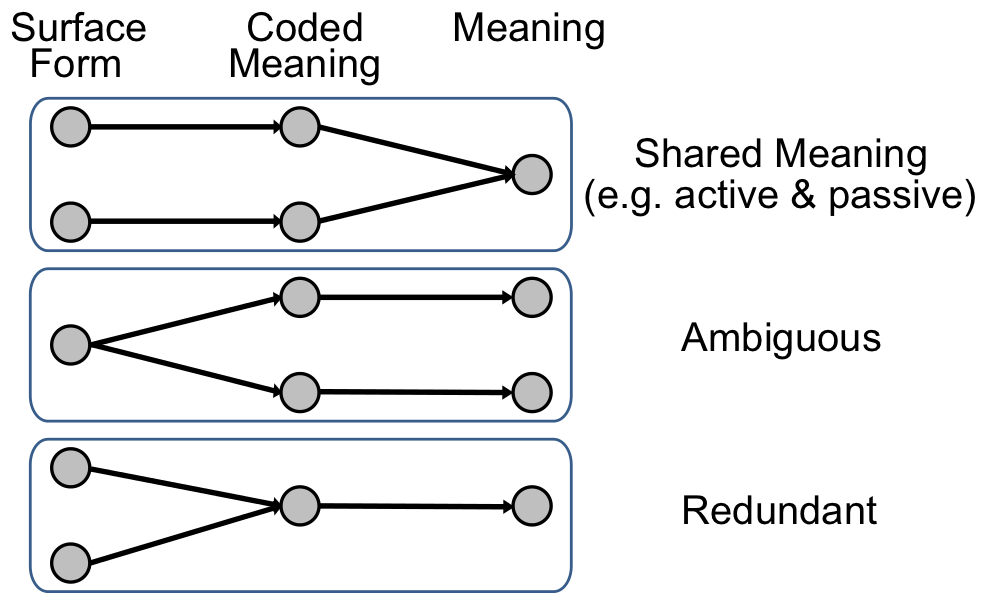
\includegraphics[width=0.8\linewidth]{meaning_relations}
\caption[Different type of sentence structure to meaning relations] {\textbf{Relation between surface form and meanings:} Sentence structure to meaning mapping exist in three categories. Active and passive sentence like "John chased the dog" and "The dog was chased by John" have the different surface form but share the same meaning i.e. chased(John, dog). Also the coded meaning of both these sentences are different i.e. SW-3 ("dog") in the active form is the 'object' whereas in passive form SW3 ("John") it is an 'agent'. Ambiguous sentences have the same surface form but different meaning and coded meaning whereas redundant sentences have different surface form but same meaning and coded meaning. Adapted from \cite{end-to-end}}
\label{fig:meaning_realtions}
\end{figure}

\paragraph{Example 1: Ambiguous Sentences}

\begin{enumerate}[noitemsep]
\item take (SW-1) the blue (SW-2) box (SW-3) \label{eg-1:sent-1}
\item take (SW-1) the left (SW-2) box (SW-3) \label{eg-1:sent-2}
\item throw(SW-1) the green(SW-2) box(SW-3)  \label{eg-1:sent-3} 
\end{enumerate}

All the three sentences having the same surface form after transforming the sentence by replacing the semantic words with 'SW' token i.e. SW the SW the SW SW.

\paragraph{Training with Sentence \ref{eg-1:sent-1}:} In the Sentence \ref{eg-1:sent-1} there are three semantic words namely SW-1: take, SW-2: blue, SW-3: box. During the training the sentence is input to the model from left to right word by word at each time step. The teacher output (thematic roles) of each semantic word is also teacher-forced as described below where, A: Action, O: Object, C: Color, I: Indicator. During the training ESN learns that second semantic word represents a \textit{'Color'}.

\begin{table}[hbtp]
\centering
\begin{minipage}{1.5in}
\begin{tabular}{|c|c|c|c|}
\hline
\multicolumn{4}{|c|}{\textbf{SW-1}}   \\ \hline
\textit{\textbf{A}}    & O & C & I 	\\ \hline
\textit{\textbf{take}} &   &   &  		\\  \hline
\end{tabular}
\end{minipage}
\begin{minipage}{1.5in}
\begin{tabular}{|c|c|c|c|}
\hline
\multicolumn{4}{|c|}{\textbf{SW-2}}                    \\ \hline
A	& O & \textit{\textbf{C}}    & I  \\ \hline
	&   & \textit{\textbf{blue}} & 	\\ \hline
\end{tabular}
\end{minipage}
\begin{minipage}{1.5in}
\begin{tabular}{|c|c|c|c|}
\hline
\multicolumn{4}{|c|}{\textbf{SW-3}}                                  \\ \hline
A	& \textit{\textbf{O}}   & C	& I \\ \hline
 	& \textit{\textbf{box}} &  	&   \\ \hline
\end{tabular}
\end{minipage}
\end{table}

\paragraph{Training with Sentence \ref{eg-1:sent-2}:} In the Sentence \ref{eg-1:sent-2} we have three semantic words; SW-1: take, SW-2: left, SW-3: ball. Both the sentences (\ref{eg-1:sent-1} and \ref{eg-1:sent-2}) differs only in the second semantic word. Now suppose we train this sentence with a teacher output as follows where symbols A, O, C and I have the same meaning as described above.

\begin{table}[hbtp]
\centering
\begin{minipage}{1.5in}
\begin{tabular}{|c|c|c|c|}
\hline
\multicolumn{4}{|c|}{\textbf{SW-1}}   \\ \hline
\textit{\textbf{A}}    & O & C & I \\ \hline
\textit{\textbf{take}} &   &   &  \\  \hline
\end{tabular}
\end{minipage}
\begin{minipage}{1.5in}
\begin{tabular}{|c|c|c|c|}
\hline
\multicolumn{4}{|c|}{\textbf{SW-2}}                    \\ \hline
A       & O & C    & \textit{\textbf{I}} \\ \hline
 &   &  & \textit{\textbf{left}} \\ \hline
\end{tabular}
\end{minipage}
\begin{minipage}{1.5in}
\begin{tabular}{|c|c|c|c|}
\hline
\multicolumn{4}{|c|}{\textbf{SW-3}}                                  \\ \hline
A                  & \textit{\textbf{O}}   & C                  & I \\ \hline
 & \textit{\textbf{box}} & \textit{\textbf{}} &   \\ \hline
\end{tabular}
\end{minipage}
\end{table}

As both the sentences used for training have the same surface form, the ESN learning from the sentence \ref{eg-1:sent-1} is disrupted after training with sentence \ref{eg-1:sent-2}. This is because the second semantic word in the sentence \ref{eg-1:sent-2} is trained to be an \textit{'Indicator'} whereas it was trained for \textit{'Color'} in the sentence \ref{eg-1:sent-1}. Such kind of ambiguous examples having the same surface form but different coded meaning (roles assignment) and actual meaning, drops the learning ability of the model. We believe that this problem is mainly because each input words are treated as a discrete atomic symbols, which does not carry any semantic information about the input words.

\paragraph{Testing with Sentence \ref{eg-1:sent-3}:} Now, when we use the sentence \ref{eg-1:sent-3} for testing, the network suggests two pseudo probabilities for the second semantic word \textit{'green'} i.e. being an \textit{'Indicator'} and a \textit{'Color'} as shown below. It becomes difficult for the model to resolve this ambiguity and assign the appropriate role. Although the word \textit{'green'} in the test sentence \ref{eg-1:sent-3} and the word \textit{'blue'} in the training sentence \ref{eg-1:sent-1} are semantically related i.e. both are colors. The model was not able to utilize this information as words were input to the in discrete forms for training. Thus by using localist vector representation we are depriving the ESN from the semantic information carried out by a words in a language.

\begin{table}[hbtp]
\centering
\begin{minipage}{1.5in}
\begin{tabular}{|c|c|c|c|}
\hline
\multicolumn{4}{|c|}{\textbf{SW-2}}  \\ \hline
A	& O & \textit{\textbf{C(0.5)}}   & \textit{\textbf{I(0.5)}} \\ \hline
	&   & \textit{\textbf{green}} 	  & \textit{\textbf{green}} \\ \hline
\end{tabular}
\end{minipage}
\end{table}

\noindent Similary the following three sentences also have the same suface form i.e. The SW is SW to SW.

\begin{enumerate}[noitemsep,label=(\roman*)]
\item The chicken(SW-1) is cooked(SW-2) to eat(SW-3) \label{eg-1:sent-i}
\item The ball(SW-1) is given(SW-2) to John(SW-3) \label{eg-1:sent-ii}
\item The book(SW-1) is taken(SW-2) to John(SW-3) \label{eg-1:sent-iii}
\end{enumerate}

Clearly we can see that the third semantic word is a \textit{'predicate'} in Sentence \ref{eg-1:sent-i} and \textit{'noun'} in sentence \ref{eg-1:sent-ii}. Thus if network is trained on sentences \ref{eg-1:sent-i} and \ref{eg-1:sent-ii} and tested on sentence \ref{eg-1:sent-iii} the network is not able to resolve the ambiguity for semantic word SW-3, which possibly leads to wrong labelling of this word.

\paragraph{Example 2: Ambiguous and Polysemous Sentences}

\begin{enumerate}[noitemsep]
\item John (SW-1) books (SW-2) the ticket (SW-3) to London (SW-4) \label{eg-2:sent-1}
\item John (SW-1) read (SW-2) the books (SW-3) to learn (SW-4) \label{eg-2:sent-2}
\end{enumerate}

Both the above sentences share the same surface form i.e. SW SW the SW to SW.

\paragraph{Training model on sentence \ref{eg-2:sent-1}} Training the model on the first sentence, the fourth semantic word \textit{'London'} is trained to be as a \textit{location}.

\paragraph{Testing model on sentence \ref{eg-2:sent-2}} Testing the model with the second sentence, the fourth semantic word \textit{learn} will be assigned the role of a location (as network was trained for this only) whereas it is actually a \textit{predicate}. The reason for such problem is that each semantic word is considered as an unique token without taking into consideration semantics of an individual word. Hence the network could not exploit the semantic information of the words during the role assignment.

\paragraph{Issue with Polysemous words:} In the first sentence, the second semantic word \textit{books} is the predicate and describe the action of making reservation, whereas the same word (books) in the second sentence is an \textit{'object'}, and represents a book which we read. Although both words are same but they represent different meanings depending on the context. These kind of words with different meaning are also known as \textit{polysemous} words. Semantic ambiguities because of polysemous words is hard to resolve with localist vector representation where each word is treated as an unique identifier. To resolve such kind of semantic ambiguities, distributed embedding of words can be useful as they are learned using the the contextual information of words.

\subsection{Research Hypothesis}

Use of abstract form of sentence and the localist word vectors as an input to the ESN have produced the promising results for the thematic role assignment task\cite{xavier:2013:RT, tra:xavier_wermter:2014}. But the behavior of the model with the distributed word embeddings was left unexplored. Thus we hypothesize that using the distributed word embeddings (e.g. Word2Vec word embeddings) could possibly resolve the problems described in the above mentioned two examples by taking into consideration the fact that they capture and encode semantic and syntactic information of words \cite{w2v:mikolov_2013_distributed, w2v:regularities_in_word_representations}. Another advantage of distributed word embedding observed over localist vector representation is that the multidimensional distributed vector representation of semantically related words remains close in the neighborhood within words embedding space (see Fig. 3). This could possibly allow the model to learn these dynamics from the distributed representation of the words and avoid the disruption caused by semantically unrelated words (as in Example 1) in the sentences with the same grammatical constructions. Whereas this semantic grouping of words is not possible in the localist vector encoding as words are represented as discrete atomic symbols.

Consider using distributed embedding of words for both the sentences in Example 2. The distributed embedding of the word \textit{'London'} (sentence 1, Example 2) encodes that it represents a \textit{'location'} along with several other semantic information. Similarly, the distributed embedding of word \textit{'learn'} (sentence 2, Example 2) also encodes that it is a \textit{'predicate'} along with other semantic information. When these distributed embeddings are used as an input to train the network, the learning of the model may not be disrupted by the sentences having the same surface form, but different semantic words. This is because the semantic information about the word is exposed to network and learned by it. Hence, thematic roles could be assigned to the words more accurately although the sentence has the same surface form.

\cleardoublepage

\chapter{Approaching Word2Vec-$\theta$RARes Language Model} \label{approach}

So far we have seen the basisc of Word2Vec model and Echo State Network. We have also seen the functioning and possible limitation of $\theta$RARes model. In this chapter, we extend the $\theta$RARes model and propose the Word2Vec-$\theta$RARes neural language model and also a Word2Vec-ESN classifier to validate the research hypothesis.

\section{Word2Vec-$\theta$RARes Language Model} \label{sec:w2v-esn_model}

This research proposes a Word2Vec-$\theta$RARes language model for TRA task. The proposed model is inspired from the $\theta$RARes model proposed by Hinaut et al. \cite{xavier:2013:RT} for TRA task. Figure \ref{fig:model_arch} shows the architecture of Word2Vec-$\theta$RARes model. Word2Vec-$\theta$RARes model is the combination of Word2Vec model and Echo State Network (ESN). The Word2Vec model is responsible for generating the distributed embeddings of the words in the input sentences. The generated word embeddings can then used as an input to ESN, which further processes these word embeddings to learn and predict the thematic roles of all semantic words in the input sentences.

\begin{figure}[hbtp]
\centering

\includegraphics[width=0.9\linewidth]{model_arch}
\caption[Architecture of Word2Vec-$\theta$RARes model]{\textbf{Architecture of Word2Vec-$\theta$RARes model:} { \small The model, takes the words of a sentence as an input across time. Word2Vec model generates the distributed vector representation of the input word. The generated word vector is then used by ESN for further processing and learns to predict the thematic roles of the input sentence.}}
\label{fig:model_arch}
\end{figure}

\subsection{Model initialization}

Before using the Word2Vec-$\theta$RARes model for TRA task, the Word2Vec model is trained using skip-gram negative sampling \cite{w2v:mikolov_2013_distributed} approach on a general purpose dataset (e.g. Wikipedia) and the domain specific dataset. During the training of Word2Vec model, the low dimensional distributed embeddings for each word in the corpus vocabulary is learned (see section \ref{get_word_embeddings}).

To initialize the ESN, firstly, a reservoir of size $N_{x}$ composed of leaky integrator neurons and \textit{tanh} activation function is created. The input-to-hidden weights ($W^{in}$) and hidden to hidden weights ($W^{res}$) are then generated sparsely and randomly from a Gaussian distribution with mean 0 and variance 1. These weights once initialized are fixed and remains unchanged during training \cite{esn:scholarpedia:2007, esn:practical_guide}. To generate the weights sparsely, a fixed fan-out of $F_{hh}$ and $F_{ih}$ is chosen for hidden-to-hidden and input-to-hidden connections respectively. In other words, each reservoir neuron is connected to $F_{hh}$ other reservoir neurons and each input neurons are connected to only $F_{ih}$ reservoir neurons. 

\subsection{Training model}

Word2Vec-$\theta$RARes language model treats the TRA task as a prediction problem. The objective of this model is to learn and predict the thematic roles of all semantic words in the input sentence. To evaluate the performance of this model meaning error and sentence error metrics are used (see section \ref{sec:evaluation_metrics_1}). The same evaluation metrics was used to evaluate $\theta$RARes model \cite{xavier:2013:RT}. Thus it enable us to compare the performance of both Word2Vec-$\theta$RARes and $\theta$RARes model.



Figure \ref{fig:model_variant_1}), shows the neural comprehension of Word2Vec-$\theta$RARes model for thematic role assignment. Like $\theta$RARes model, a set of closed class words is created prior to training of model. During the training, the sentences are presented to the model one at a time, word-by-word across time. Before presenting a sentence to the model, all the semantic words (not in closed class set) in the sentence are identified and placed in FIFO memory stack (see fig. \ref{fig:model_variant_1}). This memory stack will be used later to decode the output coded meaning of the semantic words to the meaning of input sentence. The readout layer of the model is also teacher-forced with the coded meaning of the input sentence. The size of readout layer thus depends on the maximum number of semantic words a sentence can have in the corpus. A semantic word in a sentence can have one of the four possible roles: Predicate (P), Agent (A), Object (O), Recipient (R). For example, if the sentences in the corpus have a maximum of $N_{sw}$ semantic words then the readout layer size would be $N_{sw} \times 4 $ neurons; where each output neuron encodes the thematic role of a semantic word. The model could also take the topologically modified but equivalent coded meaning of the sentences (see fig\ref{fig:w2v_esn_nv}), where the role of each noun in a sentence is represented with respect to a verb \cite{xavier:2013:RT}. With the topologically modified coded meaning, the readout units contains $N_{noun} \times N_{verb}$, where $N_{noun}$ and $N_{verb}$ are respectively the maximum number of nouns and verbs any sentence could have in the corpus. The output neurons have an activation of 1 if the corresponding thematic roles are present for the sentence, -1 otherwise. 

The Word2Vec model receives the words from an input sentence over time and generates a word vector of $E_{v}$ dimensions which is then used as an input for the ESN. The input layer of ESN uses this word vector as input features for learning and predicting the thematic roles of the semantic words in the sentences. Thus the size of the input layer is same as the dimensionality of word vector i.e. $E_{v}$. The output ofthe reservoir is accumulated for each time step during the presentation of a sentence. The accumulated reservoir states are then linearly combined with readout activations (coded meaning of the input sentence) to learn the reservoir-to-readout ($W^{out}$) weights using linear or ridge regression. The reservoir states of ESN are reset before the presentation of the consequent sentence. Word2Vec-$\theta$RARes model can be operated in two learning modes so that it learns to extract the coded meaning of the semantic words in the sentences.

\begin{enumerate}
\setlength{\itemsep}{\smallskipamount}

\item \textbf{Sentence Continuous Learning (SCL)}: In this learning mode, learning takes place from the beginning of the sentence. In other words, the coded meaning of the input sentence is made available to model from the onset of the first word of the sentence. Thus, the regression is applied with the teacher roles from the onset of the first word in the sentence \cite{xavier:2013:RT}. \label{eg:SCL}

\item \textbf{Sentence Final Learning (SFL)}: In this mode, the learning takes places only at the end of the sentence \cite{xavier:2013:RT}. Hence, the teacher labels are only provided to the network at the end of sentence i.e. from the last word of the sentence. \label{eg:SFL}

\end{enumerate} 

\begin{figure}[hbtp]
\centering
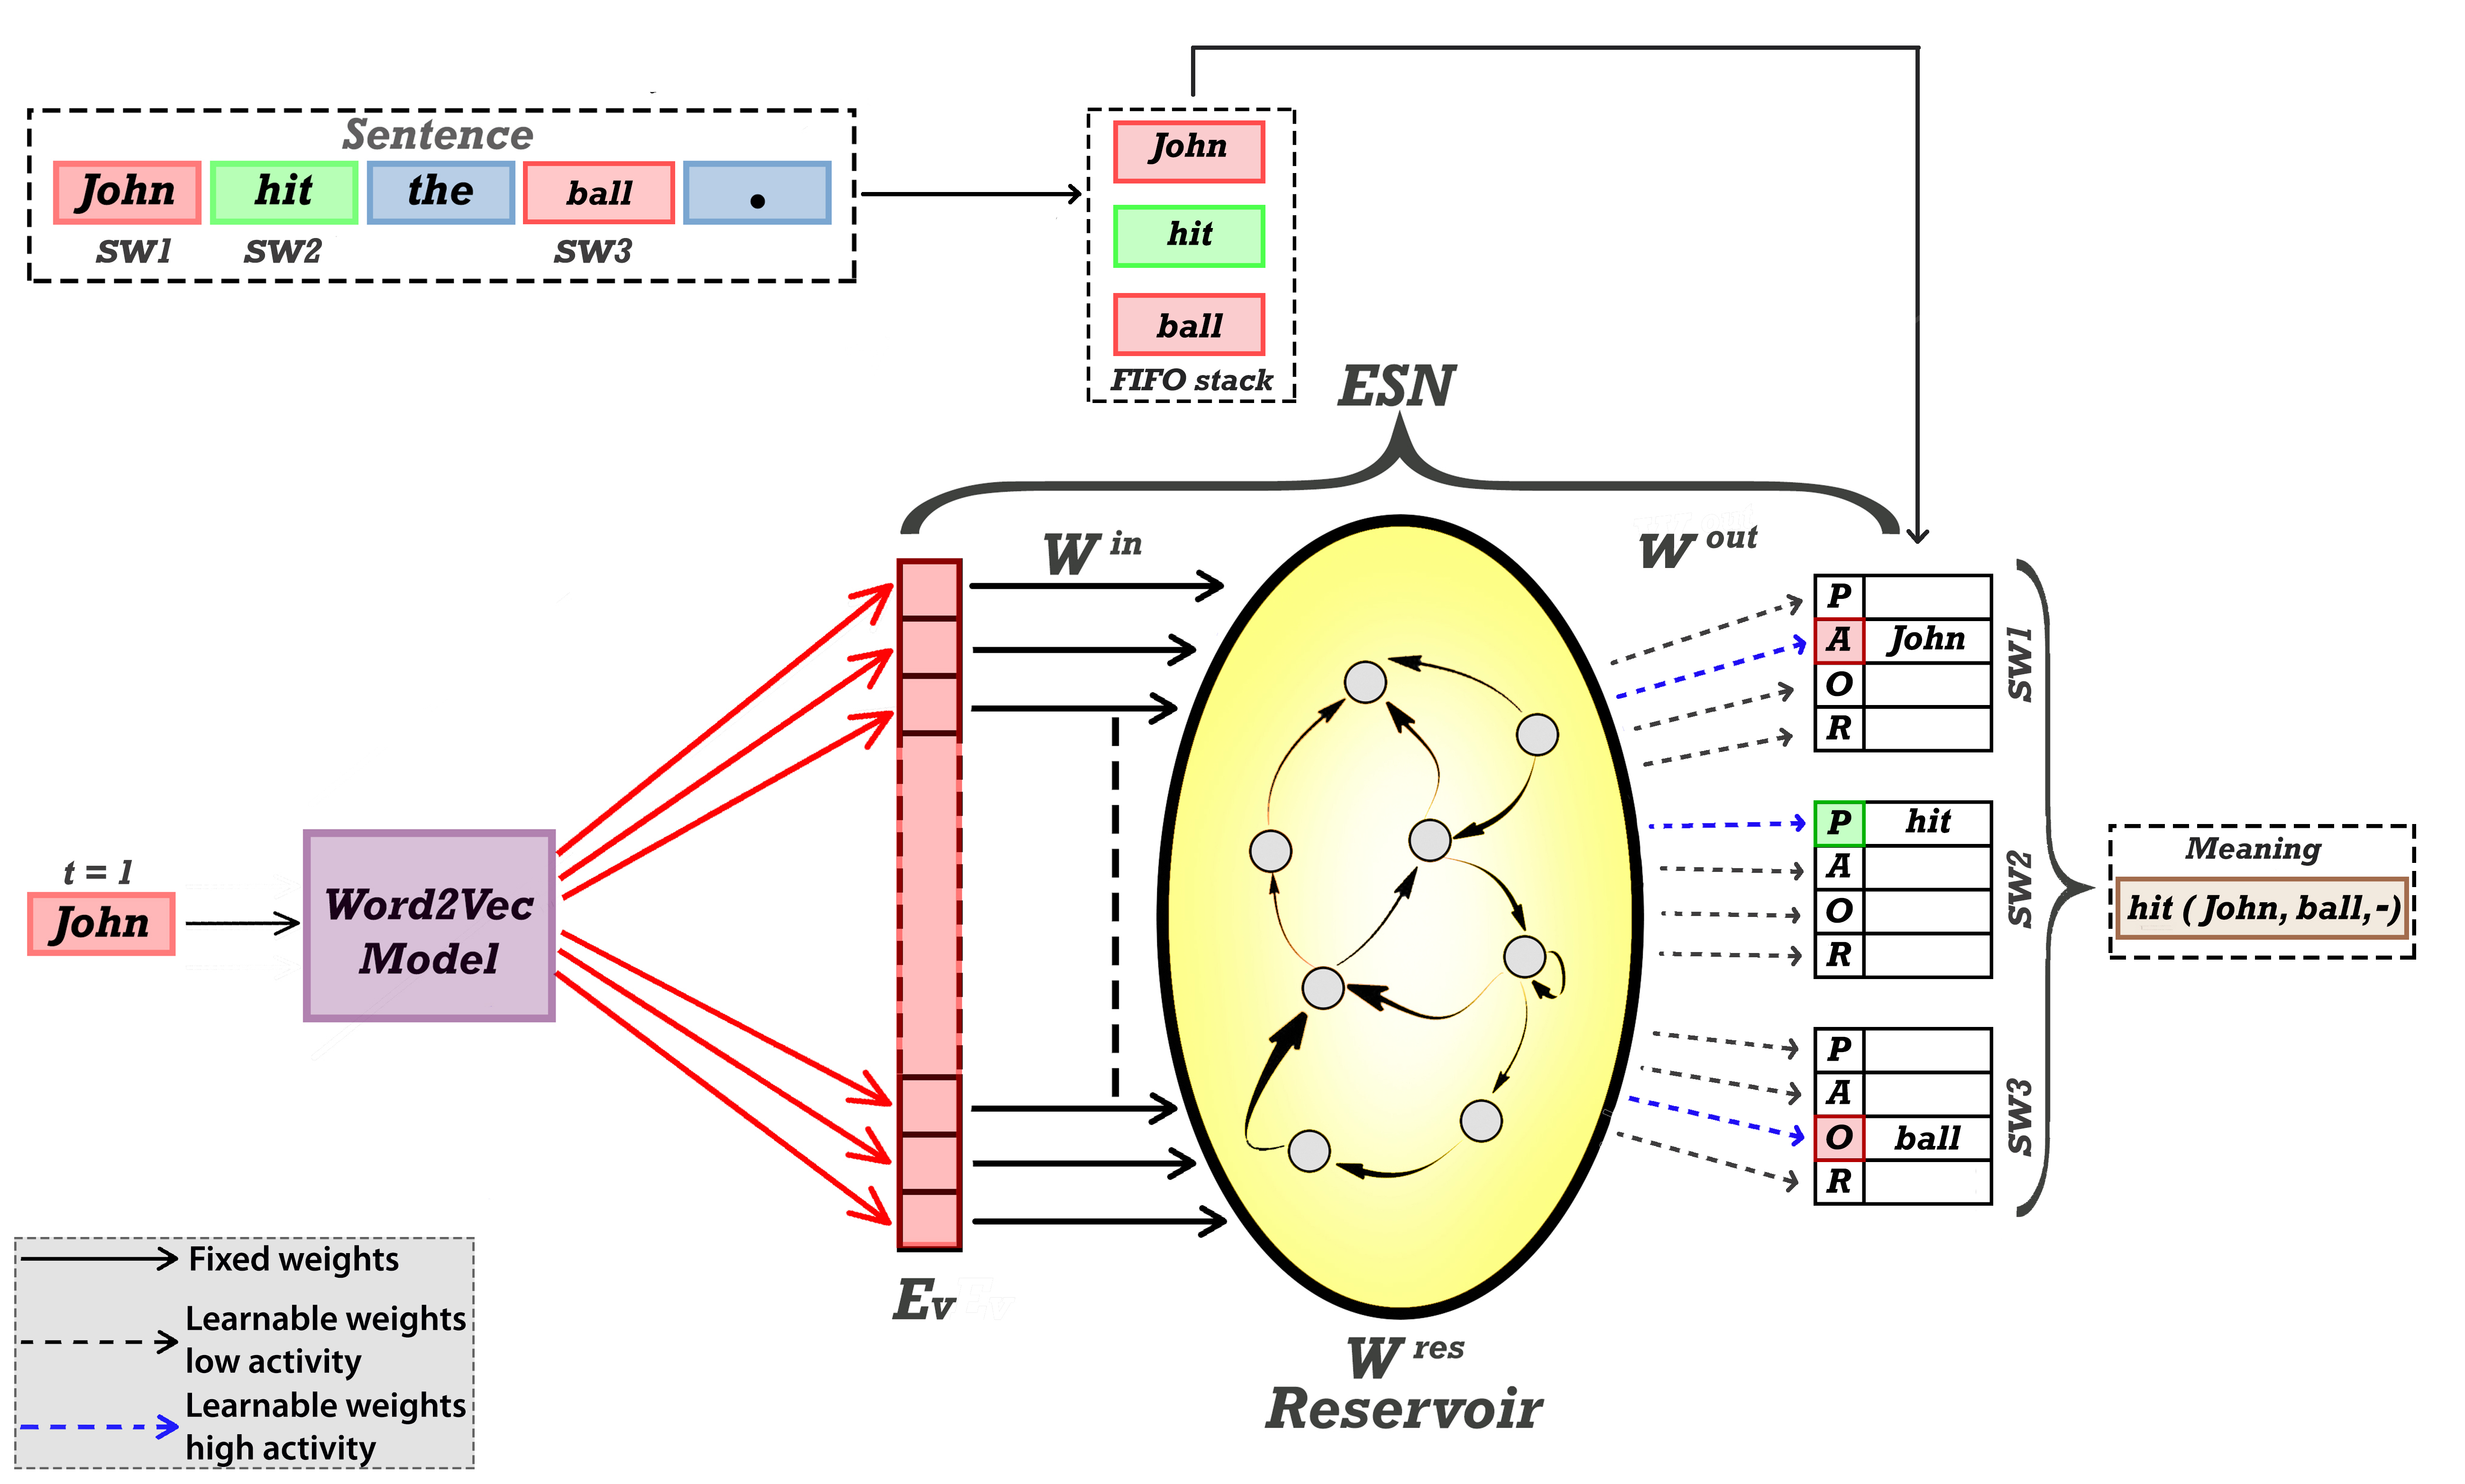
\includegraphics[width=0.9\linewidth]{w2v_esn_model}
\caption[Neural comprehension of Word2Vec-$\theta$RARes Model]{\textbf{Word2Vec-$\theta$RARes language model:} {\small The figure shows the processing of a sentence by the model Word2Vec-ESN classifier at time step 1. Nouns and verbs (specified in red and green respectively) are stored in a memory stack for interpreting the coded meaning. The word \textit{'John'} is input to word2vec model which generate a word vector of $E_{v}$ dimensions. The output vector is then input to ESN for further processing. During training, the readout units are teacher-forced with the coded meaning of the input sentence. During testing, the readout units generate the activations which code the predicted coded meaning of input sentence. The meaning: hit(John, ball, -) is decoded from coded meaning by mapping the thematic roles with semantic words from memory stack. Adapted from \cite{xavier:2013:RT}}} 
\label{fig:model_variant_1}
\end{figure}

\begin{figure}[hbtp]
\centering
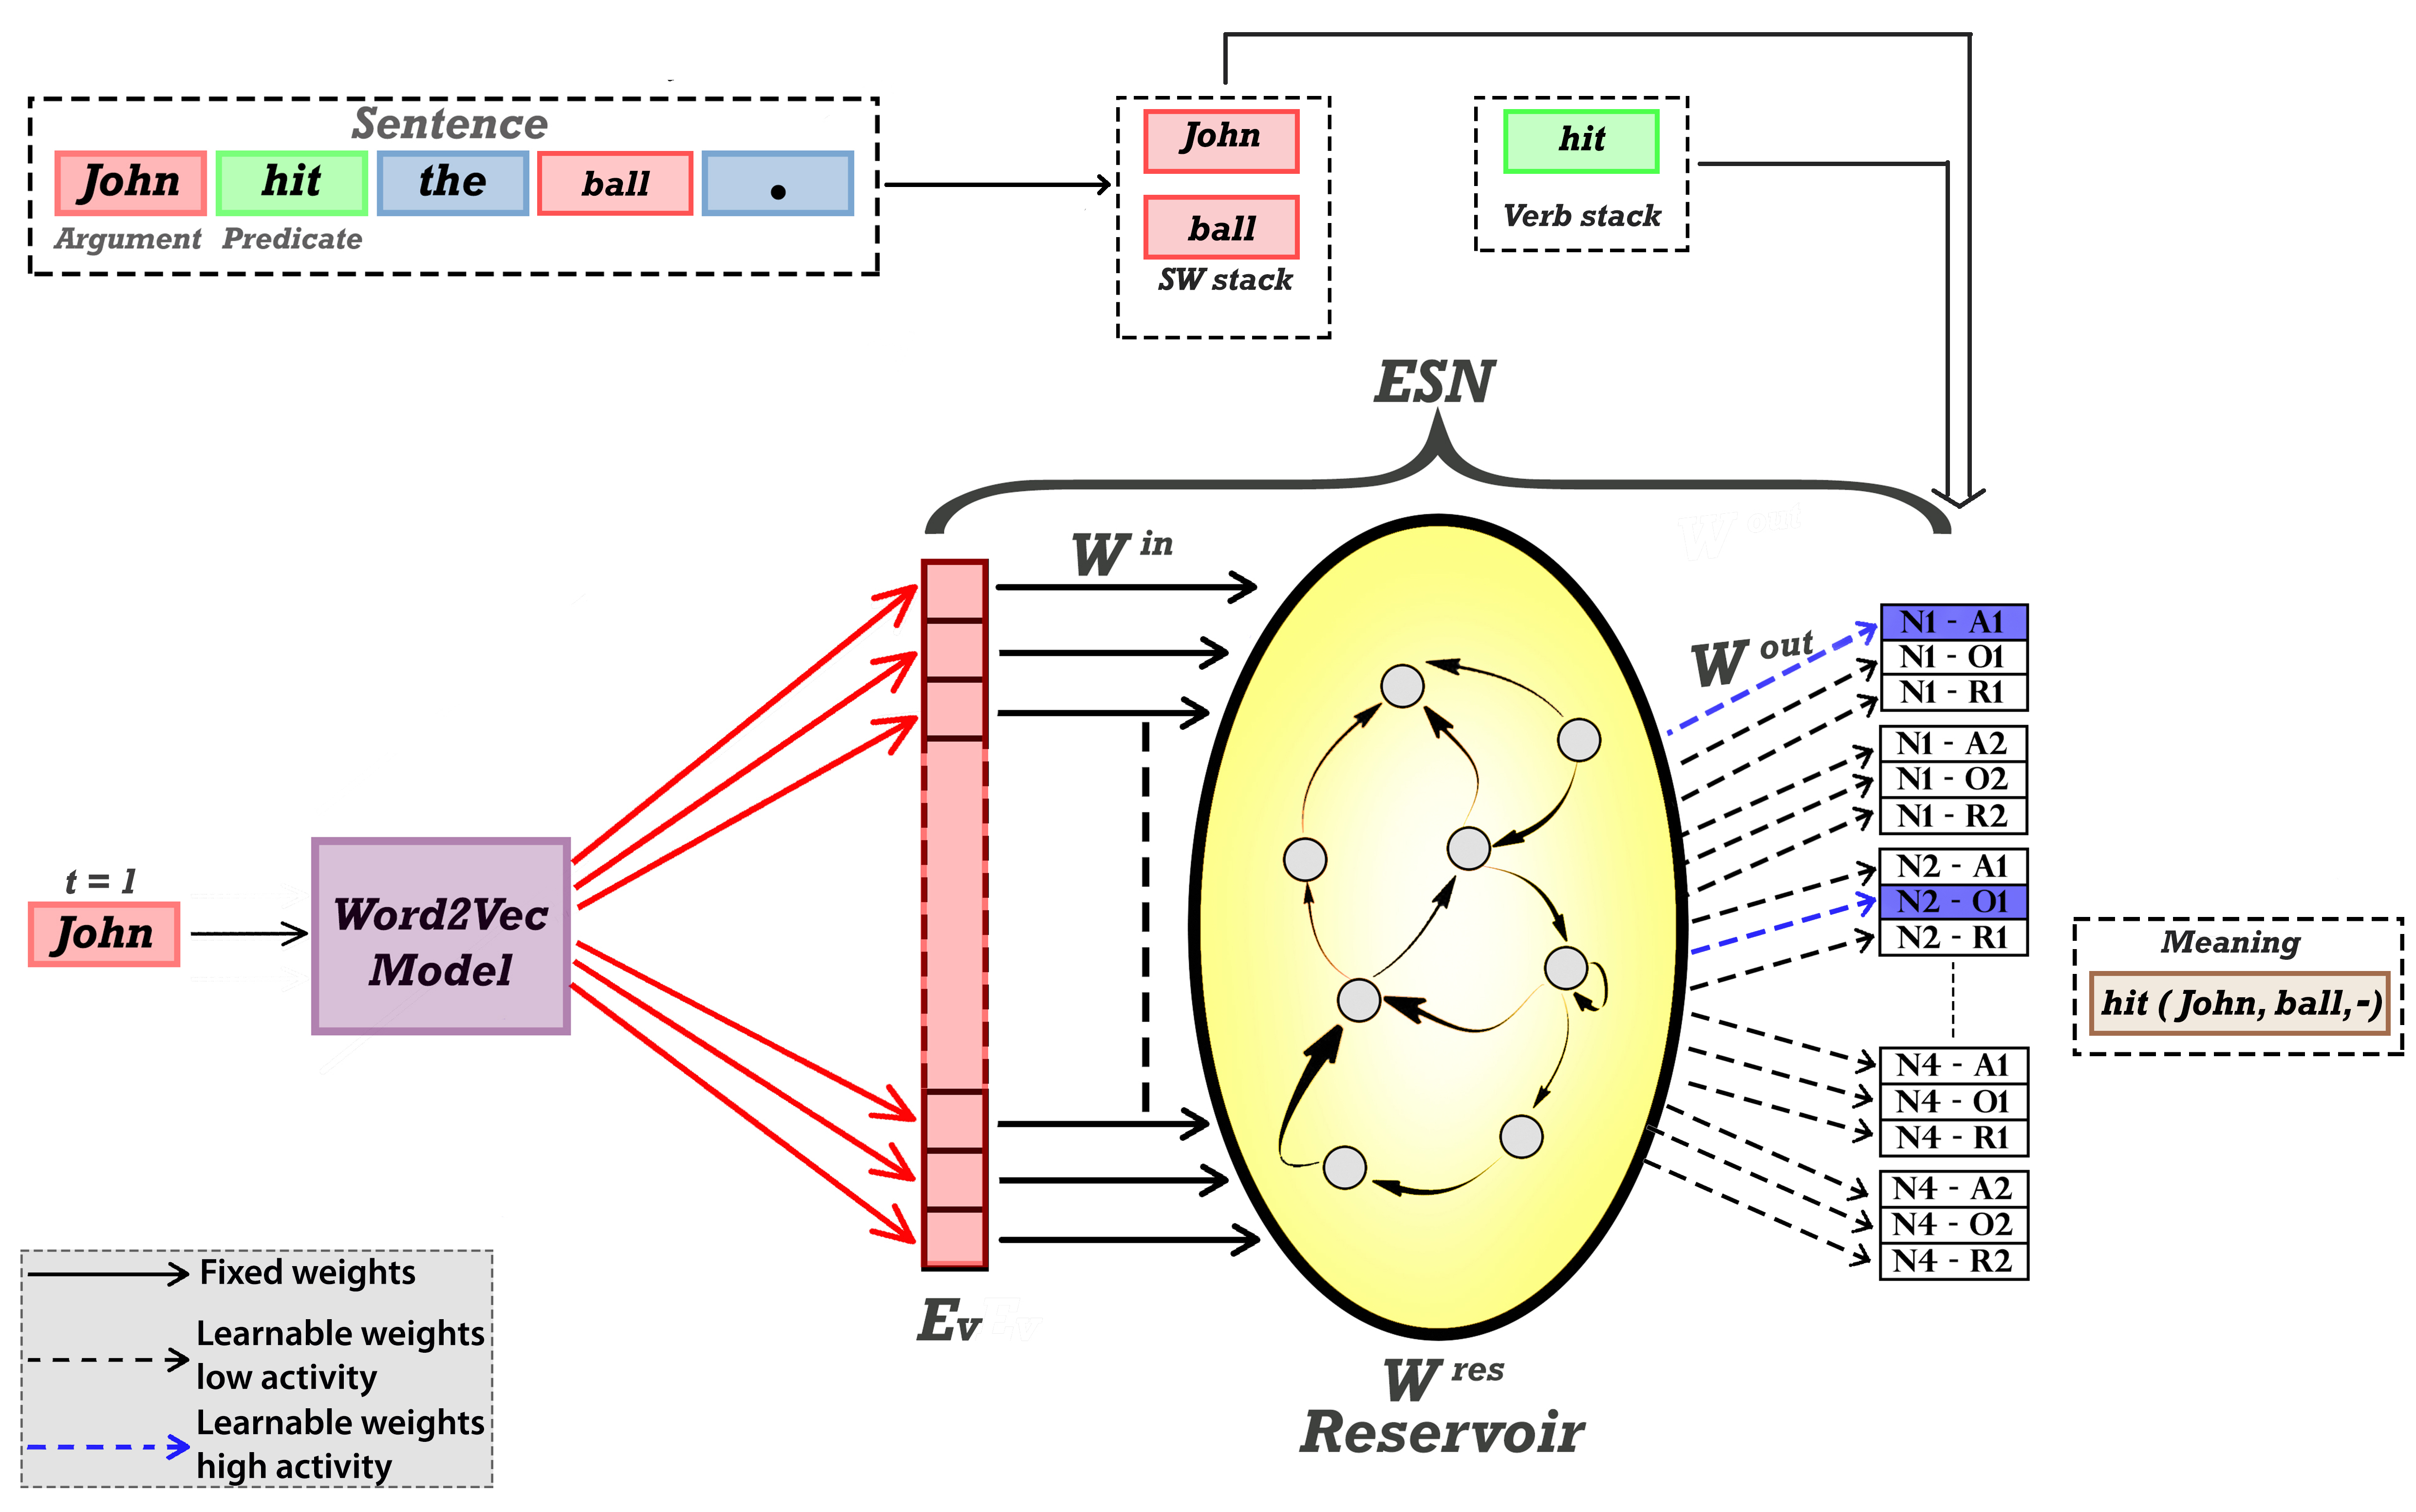
\includegraphics[width=0.9\linewidth]{w2v_esn_nv}
\caption[Neural comprehension of Word2Vec-$\theta$RARes Model]{\textbf{Word2Vec-$\theta$RARes language model with toplogically modified output coding:}{\small The figure shows the processing of a sentence by the model Word2Vec-ESN classifier at time step 1. Nouns and verbs (specified in red and green respectively) are stored in a repective memory stack for interpreting the coded meaning later. The word \textit{'John'} is input to word2vec model which generate a word vector of $E_{v}$ dimensions. The output word vector is then input to ESN for further processing. During training, the readout units are teacher-forced with the coded meaning of the input sentence. The coded meaning ``N1-A1" represents that Noun-1 (`John') is agent of Verb-1 (`hit'). During testing, the readout units generate the activations which code the predicted coded meaning of input sentence. The meaning: hit(John, ball, -) is decoded from coded meaning by mapping the thematic roles with nouns and verbs from memory stack. Adapted from \cite{xavier:2013:RT}} }
\label{fig:w2v_esn_nv}
\end{figure}

\paragraph{Decoding Output: } As described earlier, the coded meaning of a sentence is defined as the description of thematic roles for all the semantic words in the sentence. As the readout neurons of model codes the thematic roles for all semantic words, the output activations produced by the model while testing a sentence are thresholded at 0 for every semantic words. The maximum of all activation between four possible roles (i.e. Predicate, Agent, Object, Recipient) is taken as the coded meaning of a semantic word \cite{xavier:2013:RT}. A semantic word is said to have an incorrect coded meaning if the winning readout neuron is not the true role of the semantic word. If there is no activation above the threshold for a semantic word, then this semantic word is considered to have no coded meaning \cite{xavier:2013:RT}. Combining the coded meaning of semantic words, forms the coded meaning of the sentence. The coded meaning of the sentence can then be decoded to the actual meaning by mapping the coded meaning to the semantic words from the FIFO memory stack(see fig \ref{fig:model_variant_1}).
 
\subsection{Evaluation Metrics}\label{sec:evaluation_metrics_1}

To evaluate the performance of the Word2Vec-$\theta$RARes language model, the same metrics that was used by Hianut et al. \cite{xavier:2013:RT} to evaluate the $\theta$RARes model was employed. The metrics compute the Meaning Error (ME) and the Sentence Error (SE). Meaning error is the percentage of semantic words with incorrect coded meaning, whereas the sentence error is the percentage of sentences having at least one semantic word with incorrect coded meaning. Both the error measures are related, but there is no strict correlation between them \cite{xavier:2013:RT}. Sentence error is a stricter measure than meaning error to evaluate model performance because a meaning error of $5\%$ cannot be used to estimate the sentence error, as this $5 \%$ incorrect words, can be from just one sentence or several sentences. 

To evaluate the performance of Word2Vec-$\theta$RARes model, not all the readout neurons are considered i.e. if a sentence has only three semantic words then only readout neurons corresponding to these three semantic words are analyzed \cite{xavier:2013:RT} and remaining coded meaning of remaining neurons are ignored. It is important to know that if there are more than one verb, in a sentence then each semantic word can have a possible role with respect to each verb. 

\section{Word2Vec-ESN classifier}\label{sec:model_variant}

To ensure the objectivity of our findings apart from Word2Vec-ESN model, this research work also propose a Word2Vec-ESN classifier. Figure \ref{fig:model_variant_2} illustrates the functional organisation of Word2Vec-ESN classifier for TRA task. Although the model Word2Vec-ESN classifier is architecturally (see fig. \ref{fig:model_arch}) similar to Word2Vec-$\theta$RARes model, but varies in training objective and the way the sentences are processed. It treats the TRA task as a classification problem. The training objective of Word2Vec-ESN classifier is to classify the words of the input sentences to one of the roles namely Predicate (P), Agent (A), Object (O), Recipient (R) and No-role (XX) with respect to the verbs and maximize the classification scores for each role (i.e. F1-score, Precision, and Recall- see section-\ref{sec:evaluation_metrics_2}).

Two input features play a major role in Word2Vec-ESN classifier: argument and predicate. An argument describe the current word being processed and the predicate describes the verb with respect to which an argument is processed \cite{end-to-end}. So, if there are $N_{v}$ verbs in a sentence, then the same sentence is processed $N_{v}$ times. Each argument then takes a unique role for an argument-predicate pair. For example in the following sentence there are two predicates namely \textit{`chased'} and \textit{`ate'}. Thus this sentence will be processed twice, and each argument will take a role for an argument-predicate pair \cite{end-to-end}. 

\begin{table}[H]
\centering
\label{tab:argument-predicate}
\begin{tabular}{lccccccccc}
Arguments $\rightarrow$ & the & dog & that & chased & the & cat & ate & the & rat \\
Predicate('chased') 	 & XX  & A   & XX   & P      & XX  & O   & XX  & XX  & XX  \\
Predicate('ate')    	 & XX  & A   & XX   & XX     & XX  & XX  & P   & XX  & O  
\end{tabular}
\end{table}

It is worth noticing that the classifier takes in input, the predicate with respect to which an argument is processed. To retrieve the predicates from a sentence, the Word2Vec-ESN classifier has to depend on syntactic parser e.g. Charniak parser. This limits the classifier from being an end-to-end system for TRA task.  

\begin{figure}[hbtp]
\centering
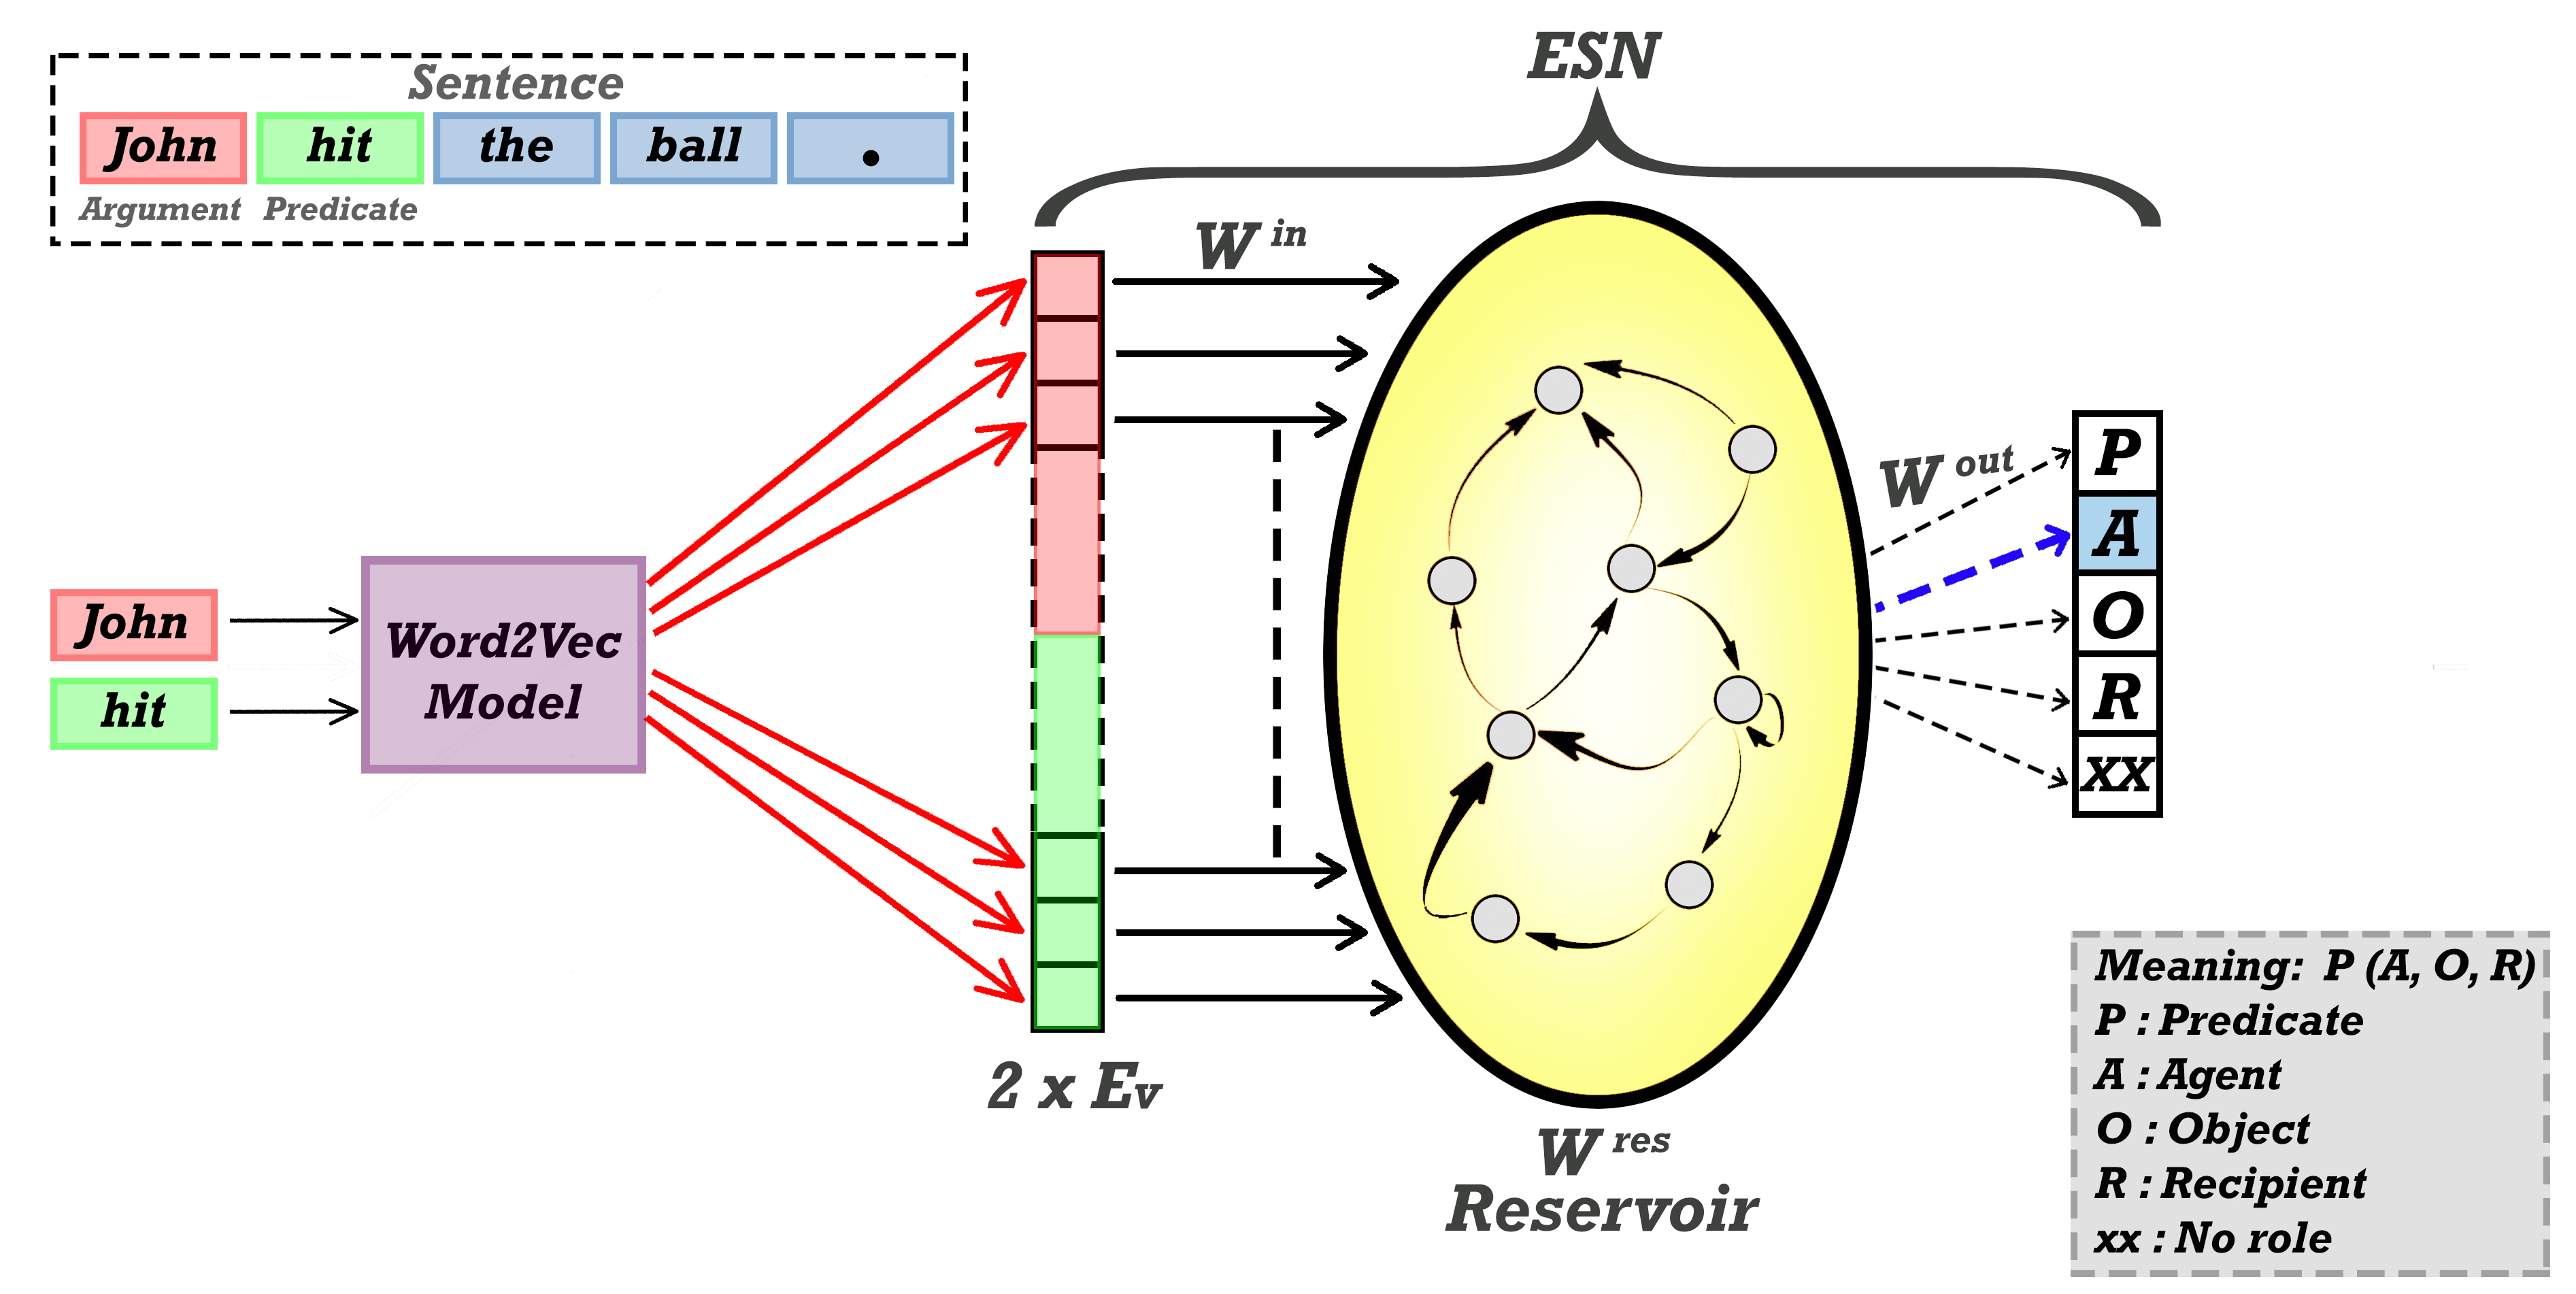
\includegraphics[width=1.0\linewidth]{w2v_esn_variant}
\caption[Functional organisation of Word2Vec-ESN classifier for TRA task] {\textbf{Functional organisation of Word2Vec-ESN classifier for TRA task:} 
{\small The figure shows the processing of a sentence in Word2Vec-ESN classifier at time step 1. At any instant of time, an argument (current word, marked in orange) and predicate (marked in green) is input to the model. Word2Vec model generates the word vectors of $E_{v}$ dimensions which are then concatenated to form a $2 \times E_{v}$ dimensions (shown in red and green color). ESN takes the resultant vector for further processing. During the training, the readout neurons are presented with the role of input word-verb pair (e.g. 'A' for Agent). The read-out weights (shown in dashed line) are learned during training. While testing, the readout unit codes the role of the semantic words, which are then accumulated and decoded to form the meaning \textit{hit(John,ball,--)} of the input sentence at the end. Inspired from \cite{xavier:2013:RT}
}}
\label{fig:model_variant_2}
\end{figure}

\subsection{Training model Word2Vec-ESN classifier}

To train the Word2Vec-ESN classifier, training sentences are presented to the model sequentially. Figure \ref{fig:model_variant_2} shows the processing of an example sentence by Word2Vec-ESN classifier. An input sentence is processed as many time as there are verbs in a sentence, forming multiple sequences. Thus the classifier takes an argument-predicate pair across the time as an input. Unlike Word2Vec-$\theta$RARes model, the readout layer has five neurons each coding for a role (P, A, O, R, XX). Thus during the training, the role of the input argument-predicate pair is also teacher-forced to the model. An output neurons have an activation 1 if an input argument-predicate pair has the corresponding role, -1 otherwise. The Word2vec model initially receives an argument-predicate pair of the input sentence and generates the distributed embeddings for both the input words. The generated word embeddings are concatenated and then taken by ESN as an input. Thus the size of ESN input layer is $2 \times E_{v}$ where the first $E_{v}$ neurons takes the vector representation of the argument and remaining $E_{v}$ neurons for the predicate. The reservoir internal states are collected for an input sequence over time. Reservoir-to-readout ($W^{out}$) weights are then learned by using the linear or ridge regression on collected reservoir states and the readout activations. 

\subsection{Decoding Output}

Recall that the Word2Vec-ESN classifier process a sentence as many times as there are verbs in the sentence. Thus while testing, the output activations of the model is used to predict the role for an argument-predicate pair. The role having the highest output activation is considered as the role of an argument-predicate pair \cite{survey_multi_class}. The role for all argument-predicate pairs is collected and the meaning of the sentence with respect to a verb can then be interpreted by filling up the tagged words in form ``P(A, O, R)". For example, in the sentence ``John hit the ball." as shown in figure \ref{fig:model_variant_2}, the roles for each word-verb pair (i.e. P, A, O, XX ) is used to deduce the meaning of the sentence as ``hit(John, ball, --)".

\subsection{Evaluation Metrics}\label{sec:evaluation_metrics_2}

To analyze the performance of this Word2Vec-ESN classifier on TRA task, the confusion matrix or contingency table \cite{confusion_martrix:1998} is used and the classification scores: Accuracy, Precision, Recall, and F1-Score, are calculated for all possible roles. Higher the classification scores the better. To get the classification score of the model, scores of individual roles are macro-averaged, to get single real numbered scores. The reason for choosing macro-average is that it gives equal weights to all the roles, addressing the role imbalance problem \cite{macro_average:2005}. The same evaluation metrics was also used for CoNLL-04 and CoNLL-05 semantic role labeling shared task \cite{conll:2004,conll:2005}.

\begin{table}[H]
\centering
\caption{Confusion matrix to evaluate Word2Vec-ESN classifier on TRA task.}
\label{tab:argument-predicate}
\begin{tabular}{l|l|c|c|c|c|c|}
\multicolumn{2}{c}{}  &\multicolumn{5}{c}{\textbf{Predicted Roles}}\\
\cline{3-7}
\multicolumn{2}{c|}{} & \textbf{A} & \textbf{O} & \textbf{R} & \textbf{P} & \textbf{XX}\\
\hhline{|~|*6-|}
\multirow{5}{*}{\textbf{True Roles}}
& \textbf{A}     & \cellcolor{gray!25}$TP_{A}$ & $E_{A-O}$ & $E_{A-R}$ & $E_{A-P}$ & $E_{A-XX}$ \\
\hhline{~|*6-}
& \textbf{O}     & $E_{O-A}$ &\cellcolor{gray!25} $TP_{O}$ & $E_{O-R}$ & $E_{O-P}$ & $E_{O-XX}$ \\
\hhline{~|*6-}
& \textbf{R}     & $E_{R-A}$ & $E_{R-0}$ & \cellcolor{gray!25}$TP_{R}$ & $E_{R-P}$ & $E_{R-XX}$ \\
\hhline{~|*6-}
& \textbf{P}     & $E_{P-A}$ & $E_{P-0}$ & $E_{P-R}$ & \cellcolor{gray!25}$TP_{P}$ & $E_{P-XX}$ \\
\hhline{~|*6-}
& \textbf{XX}     & $E_{XX-A}$ & $E_{XX-O}$ & $E_{XX-R}$ & $E_{XX-P}$ & \cellcolor{gray!25}$TP_{XX}$ \\
\hhline{~|*6-}
\end{tabular}
\end{table}

The confusion matrix describes the predictions made by the model. The rows of the matrix correspond to the actual roles and the columns correspond the predictions made by the model. The top left to bottom right diagonal elements of this matrix represent the number of words for which the predicted role is equal to the actual role. So, higher the value of diagonal elements the better. The non-diagonal elements of the matrix represent the number of words which are incorrectly labeled. 

Using the confusion matrix, accuracy can be calculated as the ratio of the number of correctly labeled words to the total number of words (equation \ref{eqn:accuracy}). This accuracy measure specifies how often the classifier is correct \cite{classification_scores:2009}. 

\begin{equation}\label{eqn:accuracy}
Accuracy = \frac{\text{number of words correctly labelled}}{\text{total number of words}}
\end{equation}
 
However, accuracy measure can be distorting (because of accuracy paradox), when the dataset has words with significant role imbalance as it gives high scores to models which merely predict the most frequent class. Thus accuracy measure cannot be used alone to evaluate the performance of the model \cite{accuracy_paradox_1:2008, accuracy_paradox_2:2014}. So, additional performance measures such as Precision (P), Recall(R), and F1-score (F1) are required to evaluate the model. All these measures take a value between 0 and 1. 

\textit{Precision} is defined as the ratio of True positive (TP) to False Positive(FP) and True Positive (equation \ref{eqn:precision}). It is the measure of the accuracy of a role provided that a specific role has been predicted \cite{classification_scores:2009}.

\begin{equation}\label{eqn:precision}
Precision = \frac{\text{True Positive}}{\text{True Positive + False Positive}}
\end{equation}

From the confusion matrix above, the precision for the role Agent($A$) is be calculated as:
\[Precision(A) = \frac{TP_{A}}{(TP_{A}+E_{O-A}+E_{R-A}+E_{P-A}+E_{XX-A})}\]

\noindent \textit{Recall} is defined as the ratio of True Positive to True Positive and False Negative. It measures how good the model is in labeling the correct roles. It is also called \textit{'Sensitivity'} or \textit{'True Positive Rate'}. \cite{classification_scores:2009}.

\begin{equation}\label{eqn:recall}
Recall = \frac{\text{True Positive}}{\text{True Positive + False Negative}}
\end{equation}

Recall for the role `A', from the above confusion matrix is calculate as:
\[Recall(A) = \frac{TP_{A}}{(TP_{A}+E_{A-O}+E_{A-R}+E_{A-P}+E_{A-XX})}\]

\noindent F1-Score or (F1) is the harmonic mean of precision and recall. In other words, it represents the balance between the precision and recall. The F1-score measure takes the false positive and the false negative into consideration. This score is really useful whenever there is a class imbalance in the dataset \cite{classification_scores:2009} and is calculated as:

\begin{equation}\label{eqn:precision}
F1 = 2\times \frac{\text{Precision} \times{Recall }}{\text{Precision + Recall}}
\end{equation}

\cleardoublepage

\chapter{Experiments}\label{experiments}

This chapter presents the experimental setup and experiments performed in this research work. The rest of the chapter is organized as follows. First, we will have an overview of the corpora used to carry out the experiments. Then we describe the configuration of the model necessary to perform the TRA task with the Word2Vec-$\theta$RARes model and the Word2Vec-ESN classifier proposed in the previous chapter. We will also see the experimental setup to perform the TRA task.

\section{Corpora and pre-processing}\label{corpora}

This section describes the corpora used to perform experiments with the proposed Word2Vec-$\theta$RARes language model and Word2Vec-ESN classifier for TRA task. Firstly, we will have an overview of the corpora used for TRA task and then we will see the corpus used to train Word2Vec model.

\subsection{Corpora For TRA Task}

In order to have a fair comparison between the Word2Vec-$\theta$RARes model and  $\theta$RARes model on the TRA task, the same corpora \footnote{https://sites.google.com/site/xavierhinaut/downloads} used by Hinaut et al. \cite{xavier:2013:RT, tra:xavier_hri} with  $\theta$RARes model was utilized. Thus, the corpus-373, corpus-462, corpus-90582 containing 373, 462 and 90582 sentences respectively, were used to perform the experiments with the proposed model on TRA task. 

\paragraph{Corpus-45:} Corpus-45 is a small corpus of 45 sentences. This corpus contains the constructions in grammatical forms i.e. `N' and `V' tokens were used to represent the nouns and verbs, along with the coded meaning of each sentence. The corpus contains the constructions with different grammatical structures i.e. active, passive, object-relative, subject-relative sentences which are represented in the form:

\begin{enumerate}[noitemsep]
\item the N V the N . \# N1-A1 N2-O1
\item the N was V by the N . \# N1-O1 N2-A1
\end{enumerate}

The coded meaning of the sentences is represented after the `$\#$' token. The coded meaning `N1-A1' can be interpreted as; the first noun is the agent of the first verb. For the object and the recipient roles `O' and `R' tokens were used respectively.

\paragraph{Corpus-462 and Corpus-90582:} The sentences in the corpus-462 and corpus-90582 were generated by Hinaut et al. using a context-free grammar for English language and used for TRA task \cite{xavier:2013:RT}. Each sentence in these corpora have verbs which take one, two, or three clause elements. For example, the sentences, ``The man \textit{jumps}", ``The boy \textit{cuts} an Apple", ``John \textit{gave} the ball to Marie", have verbs with the 1 (agent), 2 (agent and object) and 3 (agent, object and recipient) clause elements respectively. The sentences in the corpora have a maximum of four nouns and two verbs \cite{xavier:2013:RT}. A maximum of one relative clause is present in the sentences; the verb in the relative clauses could take 1 or 2 clause elements (i.e., without recipient). For example, ``The dog that bit the cat chased the boy". Both the corpus-462 and corpus-90582 have the constructions in the form:

\begin{enumerate}[noitemsep]
\item walk giraffe $<\!o\!>$ AP $<\!/o\!>$ ; the giraffe walk -s . \# ['the', 'X', 'X', '-s', '.']
\item cut beaver fish , kiss fish girl $<\!o\!>$ APO , APO $<\!/o\!>$ ; the beaver cut -s the fish that kiss -s the girl . \# ['the', 'X', 'X', '-s', 'the', 'X', 'that', 'X', '-s', 'the', 'X', '.']
\end{enumerate}

Each construction in the corpus was divided into four parts. The first part describes the meaning of the sentence using the semantic words (or open class words) in order of predicate, agent, object and recipient. The second part (between `$<\!o\!>$' and `$<\!/o\!>$') describes the order of the thematic roles of semantic words as they appear in the raw sentence. The third part (between `;' and `\#') contains the raw sentence with verb inflections (i.e. `-s') and the fourth part is the abstract representation of a sentence with semantic words removed and replace with token `X' \cite{xavier:2013:RT}.

Corpus-90582 have 90582 sentences along with the coded meaning of each sentence. This corpus is redundant; multiple sentences with different grammatical structure but the same coded meaning (see fig. \ref{fig:meaning_realtions}). In total, there were only 2043 distinct coded meanings \cite{xavier:2013:RT}. This corpus also has an additional property that along with complete coded meanings of the sentences, it also have incomplete meanings. For example, the sentence ``The Ball was given to the Man” have no \textit{`Agent'}, and thus the meaning of the sentence is ``given(-, ball, man)". The corpus also contains $5268$ pair and $184$ triplets of ambiguous sentences, i.e. 10536 and 553 sentences respectively. Thus in total there were $12.24 \%$ (i.e., $ 5268 \times 2 + 184 \times 3 = 11088 $) of ambiguous sentences which have the similar grammatical structure but different coded meaning \cite{xavier:2013:RT}.

\paragraph{Corpus-373:} Apart from the corpus-462 and corpus-90582 which were artificially constructed using the context-free grammar, the corpus-373 containing real sentences collected from humans in natural language was also used. Corpus-373 includes the instructions collected from the participants interacting with a humanoid robot (iCub) in a Human-Robot Interaction (HRI) study of language acquisition conducted by Hinaut et al. \cite{tra:xavier_hri}. In the study, the robot first performs one or two actions by placing the available objects to a location (e.g. left, right, middle) and the participants observes the actions. Then the participants were asked to instruct the robot again to perform the same actions in the natural language. Thus the corpus contains 373 complex instructions to perform single or double actions with temporal correlation (see Action Performing task in Hinaut et al. \cite{tra:tra:xavier_hri} for more details). For example, the instruction ``Point to the guitar" is a one action command whereas the instruction ``Before you put the guitar on the left put the trumpet on the right" is a complex command with double actions, where the second action is specified before the first action. A list of 86 closed class words used to filter semantic words from the sentences is also provided with this corpus. Also, unlike corpus-462 and corpus-90582 this corpus does not contain verbs inflections. Thus, this data is complex enough to test the learnability and generalization of the proposed models on TRA task.

\paragraph{Pre-processing:} As described earlier, unlike the  $\theta$RARes model, the proposed models process the raw sentences. Thus the sentences in corpus-45 are manually pre-processed by replacing the token `N' and `V' with appropriate nouns and verbs such that the coded meaning of the sentence is not changed. For example, the construction ``the N V the N" was changed to ``the man pushed the ball". Recall that the corpus-462 and corpus-90582 contains the sentences where the verbs are represented along with inflections (suffixes ``-s", ``-ed", ``-ing"). So these constructions in corpus-462 and corpus-90582 were processed to obtain the raw sentences without verb inflections. Firstly, all the words are lowercased and then the verbs with inflections are replaced by conjugated verbs \footnote{service used to find verb conjugations: \text{http://www.scientificpsychic.com/cgi-bin/verbconj2.pl}}. The verb conjugation to be used depends on the inflection used for the verb. For example, the sentences ``The giraffe walk -s" and ``John eat -ed the apple" has been changed to ``The giraffe walks" and ``John ate the apple" respectively. This preprocessing was done because the distributed word representation captured by Word2Vec model already captures these syntactic relations which was imposed previously using verb inflections e.g $vector('walks') - vector('walk') \approx vector('talks') - vector('talk')$. 
 
\subsection{Corpus For Training Word2Vec Model}

In this work, to train the Word2Vec model, a general purpose dataset i.e. Wikipedia corpus \footnote{https://dumps.wikimedia.org/enwiki/latest/} ($\approx$ 14 GB) was used to obtain the low dimensional distributed embeddings of words. The corpus contains 2,65,8629 unique words. The reason for choosing the Wikipedia dataset to train the model is that it contains most of the words used in the English language. Also, the Word2Vec model does not give good quality vector representation for words when trained over a small corpus thus a general purpose data set with billions of words is required to have better word embeddings. Thus more words we have the better the vector representation of words. Once the vector representation of words in the Wikipedia dataset is obtained, the model can then be trained further on our domain specific dataset (corpus-462 and corpus-90582) with more bias toward domain specific dataset to update the previously learned vector representations. 

\section{Models Configuration for TRA task}

In this section, we will see the necessary configuration required for the proposed model. Both the Word2Vec-$\theta$RARes and Word2Vec-ESN classifier are initialized in the same way as described in the following subsections.

\subsection{Obtaining Word Embeddings} \label{get_word_embeddings}

Before using the proposed models for TRA task, the distributed embeddings of the words are required to be learned by Word2Vec model. To get the vector representation of words, the Word2Vec model is first trained on the Wikipedia dataset using skip-gram negative sampling approach (see Chapter \ref{basics} for more details). Skip-gram negative sampling approach was used because it was claimed to accelerate the training of the model and the resultant word vectors performs better on word analogy task\cite{w2v:mikolov_2013_efficient, w2v:mikolov_2013_distributed}. 

To obtain the word vectors of different dimensions, six different Word2Vec models were trained. The hidden layers of each model contain 20, 30, 50, 100, 200, 300 neurons respectively. Thus each model produces the distributed word vectors corresponding to the size of the hidden layer. All the six models were trained using the same hypermeters as follows. A context window of $\pm 5$ for the current input word was used. The negative sampling size of 5 was chosen i.e. 5 noise words are chosen randomly from the vocabulary which does not appear in the context of the current input word. Additionally, the most frequent words are discarded with the probability using equation \ref{eqn:subsampling} with a subsampling threshold of $t = 10^{-5}$. All the words which appear less than $5$ times in the corpus were also ignored. To update the network weights stochastic gradient descent was used \cite{w2v:parameter_learning, w2v:mikolov_2013_distributed} with initial learning rate of $\alpha = 0.025$, which drops to $min_alpha = 0.0001$ linearly as training progress. 

The word embeddings obtained by training the Word2Vec model on Wikipedia dataset are accurate enough to capture the semantic relationship of the words for e.g. $vec(`Paris') -vec(`France') + vec(`Germany') \approx vec(`Berlin')$. Before training the model on Wikipedia corpus, a vocabulary of words in the corpus is created. Once the vocabulary is created, and the model is trained, it was not possible to add new words to this vocabulary. However, there is a possibility that when a domain specific corpus (e.g. corpus-462, corpus-373, etc.) is used to further train the Word2Vec model, some of the words may not be present in previously generated vocabulary. Due to this limitation, it was not possible to get the distributed embeddings of these new words. Thus we needed to update the vocabulary of the model if some words are not already present in the vocabulary to facilitate the online training of Word2Vec model. Unfortunately, neither the C++ API \footnote{https://code.google.com/archive/p/word2vec/} nor the Gensim python API \cite{w2v:gensim_api} implementation of Word2Vec model supports the vocabulary update, once created. So, we implemented the online training \footnote{The code is adapted from- http://rutumulkar.com/blog/2015/word2vec} of Word2Vec by modifying and extending the Gensim API. The new words that were not present in the existing vocabulary can now be added and initialized with some random weights, and the model can then be trained in the usual manner to learn the distributed embeddings of new words. Although now the vocabulary can be updated in an online manner, the vector embeddings of the newly added words have poor quality if their count in the new corpus is less. Thus, to have more impact of the domain specific corpus on the words embeddings and to improve the quality of words vectors, the domain specific dataset was repeated several times before training the model \footnote{Idea discussed on: https://groups.google.com/forum/$\#$!topic/gensim/Z9fr0B88X0w}.

So now when we have an online version of training the Word2Vec model, the training of Word2Vec model can be resumed on the domain-specific corpora (corpus-462 and corpus-90582). While updating the model on the new dataset, no word was disregarded irrespective of its count in the corpora. This allows us to have the vector embeddings of all the words in our domain specific corpora. Once the Word2Vec model is trained, the generated word embeddings were normalized using L-2 norm before using them for TRA task. One important point to remember while training word2vec model is that if an already trained model has to be trained further on any other corpus, then normalization should not be done, as it is not possible to train the model again with normalized word vectors \cite{w2v:gensim_api}. The trained Word2Vec model is now ready to be used with the Word2Vec-$\theta$RARes model and Word2Vec-ESN classifier.

\subsection{ESN reservoir initialization}

The size of the reservoir is one of the critical parameters of ESN and it is often recommended to use a bigger reservoir that can be computationally afforded, provided the appropriate regularization method is used \cite{esn:practical_guide}. Thus for the proposed models, a reservoir of 1000 (until and unless specified) leaky integrator neurons with \textit{tanh} activation function was used. The input-to-hidden ($W^{in}$), hidden-to-hidden ($W^{res}$) weights were randomly and sparsely generated using a normal distribution with mean 0 and variance 1. For the TRA task, output-to-reservoir weights ($W^{back}$) was not used. The reservoir state update equations \ref{eqn:res_update} and \ref{eqn:res_state} thus changes to:

\begin{equation} \label{eqn:res_new_update}
x'(n) =\textit {tanh } ( W^{res}x(n-1) + W^{in}.u(n))
\end{equation}
\begin{equation} \label{eqn:res_new_state}
x(n) =\textit (1-\alpha) x(n-1) + \alpha x'(n)
\end{equation}

To generate the sparse weights a fixed fanout number of $F_{hh} = 10$ and $F_{ih} = 2$ was used i.e. each reservoir neuron was randomly connected to $10$ other reservoir neurons and each input neuron was connected to only $2$ other reservoir neurons respectively. Use of the fixed fanout number scales the computational cost of reservoir state update linearly with increase in reservoir size \cite{esn:practical_guide}. After the weights initialization, there are several other reservoir parameters which are to be optimized and are task specific. In the next subsection, we will see how these parameters are optimized.

\subsection{Learning ESN parameters} \label{grid_search}

Echo state network have several parameters to be optimized for the proposed models to perform efficiently on the TRA task. Some of the parameters like reservoir size, sparsity, distribution of non-zero weights are straightforward \cite{esn:practical_guide}. Whereas other parameters like Spectral Radius (SR), Input Scaling (IS) and Leak Rate (LR) are task dependent and are often tuned by multiple trials. Thus to identify these parameters for TRA task, a grid search over the parameter space using five reservoir instances was performed. As the parameter search space can be gigantic, a broader grid with wider parameter ranges was first explored to find the optimal grid: grid with low sentence error for Word2Vec-$\theta$RARes model and high F1-Score for the Word2Vec-ESN classifier. The optimal region identified during the broader grid search was then used for the narrow search to identify the optimal parameters \cite{esn:practical_guide}. As both the proposed models process the sentences differently and have different training objectives, the ESN parameters for both the models were optimized separately. Additionally, the Word2Vec-$\theta$RARes model parameters are optimized separately for SCL and SFL mode. In this section, we will see the parameter optimization on corpus-462, as most of the experiments were performed using this corpus. 

\paragraph{Word2Vec-$\theta$RARes model:} To optimize the reservoir parameters, corpus-462 with the topologically modified coded meaning was used. The choice of using the modified coded meaning was deliberate and will be made clear later in Experiment-6. To get the optimal parameters (i.e. parameters resulting in the lowest sentence error) of Word2Vec-$\theta$RARes model, the model was trained and tested over a range of parameters using 10-fold cross-validation method. The corpus-462 with 462 sentences was randomly split into ten equally sized subsets (i.e. each subset with $\approx$ 46 sentences). The model was trained on sentences from 9 subsets and then tested on remaining one subset. This process was repeated ten times such that the model was trained and tested on all the subsets at least once. A reservoir of 1000 neurons and a fixed regularization coefficient, $\beta = 1\mathrm{e}{-6}$ for ridge regression was used. By exploring the parameter space we identified the optimal parameters as $SR = 2.4$, $IS = 2.5$ and $LR = 0.07$ in SCL mode and $SR = 2.2$, $IS = 2.3$ and $LR = 0.13$ in SFL mode. 

\paragraph{Word2Vec-ESN classifier: } For the Word2Vec-ESN classifier, the optimal parameters (i.e. parameters resulting to highest F1-Score) were identified during the grid search using the same corpus-462 and by applying 10-fold cross-validation. Keeping all the other conditions i.e. reservoir size and regularization coefficient, identical to Word2Vec-$\theta$RARes model described above, optimal parameters were identified as $SR = 0.7$ , $IS = 1.15$, $LR = 0.1$. As later in the Experiment-2, the performance of the Word2Vec-ESN classifier will also be tested on the sentences transformed to grammatical form (i.e. semantic words replaced with 'SW' token) and represented in localist fashion. Thus it is also required to find the optimal parameters for this transformed corpus. Keeping all the conditions same, the grid search was performed over parameter space and identified the optimal parameters were identified as $SR = 1.3$, $IS = 1.0$ , $LR = 0.4$. 

\subsection{Input and Output Coding}

As specified in chapter \ref{approach}, the Word2Vec-$\theta$RARes model and Word2Vec-ESN classifier process the sentences differently, thus the input and output coding for both the model also differs. However, the initialization of Word2Vec model and ESN reservoir weights remains same for both the models. 

\paragraph{Word2Vec-$\theta$RARes model:}

A raw sentence is presented to the model, where each word in the sentence is processed across time by both Word2Vec model and ESN. The Word2Vec model outputs the $E_{v} = 50$ dimension word embedding which is then used as an input for ESN. Thus input layer of ESN has $50$ neurons.

For all the experiments on corpus 45, 462 and 90582 (Experiments 1-5 in next section), an equivalent but topologically modified coded meaning (see section \ref{sec:model_variant}) was used. The readout layer of ESN contains 24 $(4 \times 3 \times 2)$ neurons as the corpus contains sentences, having a maximum of 4 nouns each having 3 possible roles (Agent, Object, and Recipient) with respect to a maximum of 2 verbs. Each neuron in the readout layer thus codes for a role of a noun with respect to a verb. The corpus-90582 contains a maximum of 5 nouns, and thus the size of readout layer is 30 $(5 \times 3 \times 2)$. 

For Experiment-6, the topologically modified coding was not used. So, the readout layer contains 36 $(6 \times 3 \times 2)$ neurons as there are maximum of 6 semantic words in this corpus and each could take one of the 3 possible thematic roles (Object, Predicate, Location) with respect to a maximum of two actions \cite{tra:xavier_hri}. Output neurons have an activation 1 if the corresponding roles are present in the sentence, -1 otherwise. 

\paragraph{Word2Vec-ESN classifier:}

Recall that in Word2Vec-ESN classifier a raw sentence is presented to the model, where each word (argument) along with the verb (Predicate) with respect to which the word is currently processed, is input to the model across time (see section \ref{sec:model_variant}). Also, A sentence is processed as many time as there are verbs in the sentence. So, the Word2Vec model takes this argument-predicate pair as an input and outputs a vector of $E_{v} = 2 \times 50$ dimension, which is then used as an input to ESN. Thus the input layer contains $100$ neurons where first $50$ neurons encodes the vector representation of the word and remaining $50$ neurons codes for the verb with respect to which word is being processed. Unlike the Word2Vec-$\theta$RARes, the size of readout layer always remains the same and contains five neurons each coding for a role: Predicate (P), Agent (A), Object(O), Recipient (R) and No Role (XX) for both corpus-462 and corpus-90582. Readout neuron of ESN has an activation 1, if the input word-verb (argument-predicate) pair have the corresponding role, -1 otherwise.

\section{Experimental Setup}

In this section we descibe the experiments performed in this thesis. Untill and unless specified we use all the optimal parameters identified during the grid search for both Word2Vec-$\theta$RARes model and its Word2Vec-ESN classifier, described in section \ref{grid_search}. 

\subsection{Experiment-1: Models performance on small corpous}\label{exp-1}

In order to see the performance of Word2Vec-$\theta$RARes model and its Word2Vec-ESN classifier on TRA task with the small corpus, the model was first tested with the limited number of sentences i.e. 26 sentences (sentence 15 to 40) from corpus-45. The chosen sentences have distinct surface form and grammatical structure (e.g. active, passive, dative-passive). Both the models were first trained and tested on all the sentences to get the training errors and then tested using Leave one Out (LoO) cross-validation method: training on 25 sentences and testing on remaining one sentence such that all the sentences are tested at least once. Reservoir parameters for this experiments were optimized on the 26 constructions used in the experiment by exploring the parameter space and using LoO cross-validation approach. This experiment remains a toy demonstration, and we will later see the generalization capability of the model with an extended corpus in Experiment-2 and Experiment-5.
 
\paragraph{Word2Vec-$\theta$RARes model:} For simulation with Word2Vec-$\theta$RARes model, five reservoir instances each with 1000 neurons and reservoir parameters $SR = 2.1$ , $IS = 6.6$, $LR = 0.5$ was used. The model was operated in SCL mode.

\paragraph{Word2Vec-ESN classifier:} For simulations with the Word2Vec-ESN classifier, five reservoir instances each with 500 neurons and reservoir parameters $SR = 0.2 $ , $IS = 0.7$ , $ LR = 0.7$, was used. 

\subsection{Experiment-2: Generalization Capabilities} \label{exp-2}

In the experiment \ref{exp-1}, we performed simulations with the limited set of sentences. Thus in order to test the generalization capability of the model, an extended corpus of 462 sentences was examined (see corpus-462 in \ref{datasets}). 

\paragraph{Word2Vec-$\theta$RARes model:} Using the extended corpus-462, generalization capability of Word2Vec-$\theta$RARes model was tested using 10-fold cross-validation approach. For this experiment, equivalent but topologically modified output coding of sentences was used for training (see fig. \ref{fig:model_variant_2}). In order to compare the generalization ability of the Word2Vec-$\theta$RARes model and  $\theta$RARes model, simulations were performed in both the learning modes i.e. in SCL and SFL mode. The reservoir parameters identified during grid search for both the learning modes were used i.e. $SR = 2.4$, $IS = 2.5$, and $LR = 0.07$ in SCL mode and $SR = 2.2$, $IS = 2.3$ and $LR = 0.13$ SFL mode (see section \ref{grid_search}). For simulations in each learning mode, five reservoir instances (i.e. reservoir weights were initialized using 5 different random generator seeds) each with a reservoir of size 1000 neurons was used.

\paragraph{Word2Vec-ESN classifier:} Recall that the Word2Vec-ESN classifier unlike Word2Vec-$\theta$RARes model evaluate the performance of model using classification metrics(see section \ref{sec:model_variant} in chapter \ref{approach}). The model process the raw sentences and the distributed vector representation of input argument-predicate pair is fed into ESN. However, it is also important to test the behavior of this model on the sentences transformed to grammatical form and using localist word representation i.e. without the word2vec unit in the model, as an input to ESN. This will allow us to have an insight on the benefits of distributed word vector. Thus for this experiment, the Word2Vec-ESN classifier was used in two configurations mentioned below. Simulations in both the configurations were performed using five reservoir instances each with a reservoir of 1000 neurons.

\begin{enumerate}
\setlength{\itemsep}{\smallskipamount}

\item \textbf{Configuration-1: } In this configuration, the Word2Vec-ESN classifier process the raw sentences and distributed vector representation of argument-predicate pairs are input to ESN (see section \ref{sec:model_variant} for more detail). For the simulation in this configuration, the reservoir parameters $SR = 0.7$ , $IS = 1.15$, $LR = 0.1$ were used. The parameters are identified previously by exploring the parameter space. \label{config-1}

\item \textbf{Configuration-2: } In this configuration, the Word2Vec-ESN classifier is used without Word2Vec unit, and only ESN is used for processing the sentences. The input sentences were transformed in the grammatical form: all the semantic words in the sentence were replaced with 'SW' token, and localist word vectors are input to ESN. For the simulation in this configuration, the reservoir parameters $SR = 1.3$, $IS = 1.0$ , $LR = 0.4$ found previously during grid search were used. \label{config-2}

\end{enumerate} 

\subsection{Experiment-3: Effect of Corpus structure} \label{exp-3}

As described earlier, that the sentences in the corpus-462 were created based on context-free grammar. Thus the sentences in the corpus contain an inherent grammatical structure. The models thus possibly utilize the underlying grammatical structure to some extent for learning and generalizing. To test this hypothesis and to demonstrate that the model is not generalizing on any other inconsistent regularity in the corpus, in this experiment, the inherent grammatical structure from the sentences was removed by randomizing the word orders within the sentences \cite{xavier:2013:RT}. Such a test will also help us to have an insight on what the model is actually learning and whether the model is overfitting or not. 

\paragraph{Word2Vec-$\theta$RARes model:}In this experiment, the corpus-462 with the scrambled sentences (i.e. in the absence of any grammatical structure) was presented to Word2Vec-$\theta$RARes model. Keeping all the conditions and the reservoir parameters same as used in Experiment-2, a 10-fold cross-validation was performed with five model instances. The cross-validation errors obtained in the Experiment-2 on the corpus-462 with inherent grammatical structure can then be compared with the cross-validation error obtained while using scrambled corpus. If the model is not overfitting and learning from the grammatical structure, then the model should not perform better on the corpus with scrambled sentences (i.e. in the absence of grammatical structure). However, in the case of overfitting the generalization effect on the corpus should not vary much both in presence and absence of grammatical structure \cite{xavier:2013:RT}. 

\paragraph{Word2Vec-$\theta$RARes model:} Like Word2Vec-$\theta$RARes model, the Word2Vec-ESN classifier was also presented with the scrambled sentences of corpus-462. Keeping all the conditions and the reservoir parameters same as used in Experiment-2, a 10-fold cross-validation was performed with five instances of the Word2Vec-ESN classifier. The Word2Vec-ESN classifier was also operated with scrambled corpus in configuration-1 and configuration-2 as described in Experiment-2.

\subsection{Experiment-4: Effect of Reservoir size} \label{exp-4}

The most important hyperparameter which affects the performance of the model is the size of the reservoir (i.e. $N_{x}$ = number of neurons in the reservoir). The addition of neurons in the reservoir is also computationally inexpensive because the read-out weights ($W^{out}$) scales linearly with the number of neurons in the reservoir \cite{esn:learn_gs}. So, in order to determine the effect of reservoir size on the performance of the Word2Vec-$\theta$RARes model and Word2Vec-ESN classifier, the simulations were performed over a range of reservoir sizes \footnote[1]{Reservoir sizes explored in Word2Vec-$\theta$RARes model: [90, 291, 493, 695, 896, 1098, 1776, 2882, 3988, 5094]} \footnote[2]{Reservoir sizes explored in Word2Vec-ESN classifier: [50, 100, 250, 400, 600, 800, 1050, 1600, 2250, 3320, 3860, 4500]} using five reservoir instances. 

\paragraph{Word2Vec-$\theta$RARes model:} With Word2Vec-$\theta$RARes model, the simulations were performed on a range of reservoir size\footnotemark[1] in both SCL and SFL modes using the same optimal reservoir parameters as used in the Experiment-2 i.e. $SR = 2.4$, $IS = 2.5$ and $LR = 0.07$ in SCL mode and $SR = 2.2$, $IS = 2.3$ and $LR = 0.13$ in SFL mode. 

\paragraph{Word2Vec-ESN classifier:} To see the effect of reservoir size on Word2Vec-ESN classifier, simulations were performed on a range of reservoir sizes \footnotemark[2], in both the configuration-1 and configuration-2 of Word2Vec-ESN classifier as described in Experiment-2. 

\subsection{Experiment-5: Scalability of the model} \label{exp-5}

In order to investigate the effect of corpus size and determine the scaling capability of the model, the extended corpus-90582 (see section \ref{corpora}) was used for this experiment. As this corpus also contains $12\%$ of ambiguous sentences which impedes the learning and generalization of the model, this experiment will also validate the model's ability to process the abmbiguous sentences. Thus, in order to study the scaling capabilty of the model with different corpus size, 6 sub-corpora were created by randomly sampling $6\%$, $12\%$, $25\%$, $50\%$, $75\%$, $100\%$ of sentences from the orginal corpus of 90582 sentences \cite{xavier:2013:RT}.

\paragraph{Word2Vec-$\theta$RARes model:} Each of the generated sub-corpora was exposed to the Word2Vec-$\theta$RARes model, and a 2-fold cross-validation was performed. The model was trained on half the sub-corpora size and tested on remaining half. The second half used for testing was then used to train the model and tested on the first half, used for training previously. This experiment was performed with the Word2Vec-$\theta$RARes model in both the learning modes i.e. SCL and SFL mode, using five reservoir instances each with 5000 neurons. All the other parameters were kept identical to the Experiment-2. 

\subsection{Experiment-6: Generalization on new corpus} \label{exp-6}

One may argue that the previously used corpora (corpus-462 and corpus-90582), which were artificially constructed using context-free grammar may add a bias to the model. Thus making it easier for the model to learn and generalize on these corpora for TRA task. To answer this question, in this experiment, the corpus-373 (see section \ref{corpora}) containing the instructions collected from humans in a Human-Robot Interaction (HRI) study of language acquisition was used. 

\paragraph{Word2Vec-$\theta$RARes model:} To test the generalization of Word2Vec-$\theta$RARes model on corpus-373, the model was operated in SCL mode and tested using the LoO cross-validation method. The SCL mode and the LoO method were chosen so that results of this experiment can be compared with that of obtained using  $\theta$RARes model \cite{tra:xavier_hri}. Also, to make the results of both the model deterministically comparable, topologically modified coding was not utilized for this experiment (see section \ref{sec:w2v-esn_model}) and simulations were performed using ten reservoir instances. 

For this experiment, reservoir parameter space was not explored to identify optimal reservoir parameters, but instead, the previously optimized parameters obtained on corpus-462 with topological modified coded meaning was used i.e. $SR = 2.4$, $IS = 2.5$ and $LR = 0.07$ (see section \ref{grid_search}). Doing so will enable us to test the robustness of these model parameters on the new corpus i.e. corpus-373.

\subsection{Experiment-7: Effect of Word2Vec word dimensions} \label{exp-6}

In all the previous experiments, the distributed word vectors of 50 dimension were used. Mikolov et al. \cite{w2v:mikolov_2013_efficient, w2v:mikolov_2013_distributed} showed that the word vectors of higher dimensions (e.g. 300 in their case) perform better on word analogy task. Thus in this experiment, the effect distributed word vector dimensions on the TRA task will be explored. This experiment was only performed on Word2Vec-$\theta$RARes language model.

\paragraph{Word2Vec-$\theta$RARes model:} Recall that in section \ref{get_word_embeddings}, six Word2Vec models were trained to generate the word vectors of 20, 30, 50, 100, 200, 300 dimensions respectively. To test the effect of these word vector dimensions on TRA task, each of these Word2Vec model was used in Word2Vec-$\theta$RARes language model. For this experiment, the corpus-373 without the topologically modified coded meaning was used (see fig. \ref{fig:model_variant_1}). Simulations were performed using ten reservoir instances each with 1000 neurons. The model was trained and tested using LoO cross-validation approach in both the SCL and SFL mode, and all the reservoir parameters were kept identical to Experiment-2.

\cleardoublepage

\chapter{Experiments and Results}\label{results}

This chapter summarizes the experiments performed with the proposed model described in chapter \ref{approach}. In total, seven experiments were performed using the corpora outlined in the previous chapter. Along with the experiments, the results are also presented and compared with that of obtained using $\theta$RARes model wherever required. 

\section{Experiment-1: Performance on Small Corpus}

In order to see the performance of Word2Vec-$\theta$RARes model and Word2Vec-ESN classifier with the small corpus on the TRA task, the models were first tested with a limited number of sentences i.e. 26 sentences (sentence 15 to 40) from corpus-45. The chosen sentences have the distinct surface form and grammatical structure (e.g. active, passive, dative-passive). Using five instances of both the models, each model was first trained and tested on all the sentences to get the training errors and then tested using Leave one Out (LoO) cross-validation method: training on 25 sentences and testing on remaining one sentence such that all the sentences are tested at least once. Reservoir parameters for this experiments were optimized on 26 constructions used in the experiment by exploring the parameter space and using LoO cross-validation approach. This experiment remains a toy demonstration, and the generalization capability of the model will be investigated later with an extended corpus in Experiment-2 and Experiment-5.

\begin{table}[htbp]
\centering
\begin{threeparttable}
\caption[Cross-Validation errors with Word2Vec-$\theta$RARes on limited number of sentences.]{Generalization errors in SCL mode on 26 sentences of corpus-45.}
\label{tab:corpus_45_errors}
\rowcolors{2}{gray!25}{white}
\begin{tabular}{llcc}
\toprule
                           &              &  Word2Vec-$\theta$RARes     & $\theta$RARes \\
\midrule                 
\textbf{Meaning Error}    & mean         & 35.09                      & 14.83  \\
                        & std.         & 05.89                     & 02.59  \\
\textbf{Sentence Error}    & mean         & 85.38                      & 42.73 \\
                        & std.         & 07.88                     & 07.19 \\
\bottomrule
\end{tabular}
\begin{tablenotes}
\small
\item 
LoO cross-validation errors with both Word2Vec-$\theta$RARes model and $\theta$RARes model (shown in \%). Mean and std. is the average and standard deviation of errors over several model instances.
\end{tablenotes}
\end{threeparttable}
\end{table}

\paragraph{Word2Vec-$\theta$RARes Model:} For simulation with Word2Vec-$\theta$RARes model in this experiment, the model was operated in the SCL mode. Also, the reservoir of 1000 neurons and parameters $SR = 2.1$, $IS = 6.6$, $LR = 0.5$ were used. When trained and tested on all the 26 sentences, the model learned the sentences without any errors. However, during the cross-validation the model failed to generalize and yielded high cross-validation error rates (ME = $35.09\%$ and SE = $85.38\%$). This indicates that the Word2Vec-$\theta$RARes model is overfitting on the dataset. However, this is not surprising because the dataset contains limited examples, which constrained the model to generalize well. 

As illustrated in Table \ref{tab:corpus_45_errors}, it can be seen that the cross-validation errors with Word2Vec-$\theta$RARes model are almost doubled when compared to $\theta$RARes model. It is also important to know that the cross-validation errors of $\theta$RARes model reported in the Table \ref{tab:corpus_45_errors} are averaged over 100 reservoir instances of 100 units each \cite{xavier:2013:RT}. Whereas, the cross-validation errors of Word2Vec-$\theta$RARes are averaged over five reservoir instances of 1000 neurons each. With the small reservoir of 100 neurons, the Word2Vec-$\theta$RARes failed to learn and generalize (not reported here) on the same 26 sentences used in this experiment. This shows that the $\theta$RARes model performs better than the proposed Word2Vec-$\theta$RARes model on the small dataset even with a small reservoir.

\paragraph{Word2Vec-ESN classifier:} For simulation with Word2Vec-ESN classifier, a reservoir of size 500 neurons and parameters $SR = 0.2 $ , $IS = 0.7$ , $ LR = 0.7$, were used. As illustrated in Table \ref{tab:corpus_45_scores}, the Word2Vec-ESN classifier learned the 26 sentences resulting in F1-Score of $95.68\%$ during the training. While testing the classifier using LoO cross-validation method it generalized with low F1-Score of $68.53\%$. The high difference in F1-Score during training and testing conditions points toward the limited generalization capability of the classifier on unseen sentences. 

\begin{table}[htbp]
\centering
\begin{threeparttable}
\caption[Generalization score with Word2Vec-ESN classifier on limited number of sentences.]{Classification score of model Word2Vec-ESN classifier on 26 sentences from corpus-45.}
\label{tab:corpus_45_scores}
\rowcolors{2}{gray!25}{white}
\begin{tabular}{llccc}
\toprule
                   &              &  Precision         & Recall    & F1-Score\\
\midrule                
\textbf{training error}    & mean         & 94.92              & 96.54     & 95.68  \\
                & std.         & 00.27             & 00.74      & 00.46  \\
\textbf{test error}    & mean         & 69.87              & 71.29      & 68.53 \\
                & std.         & 02.36             & 01.37     & 01.80  \\
\bottomrule
\end{tabular}
\begin{tablenotes}
\small
\item 
LoO classification scores of Word2Vec-ESN classifier (shown in \%). Mean and std. is average and standard deviation of classification scores over several model instances.
\end{tablenotes}
\end{threeparttable}
\end{table}


\section{Experiment-2: Generalization Capabilities} \label{exp-2}

In the previous experiment, we saw the performance of both the proposed models with a limited number of sentences. The results indicated that the model is probably overfitting and not generalizing on the unseen sentences. Therefore, in this experiment, an extended corpus of 462 sentences (see section \ref{corpora}) was used to test the generalization capability of the models. The simulations were performed with five instances of both the proposed models each with a reservoir of 1000 neurons. To test the learning ability, both the models were initially trained and tested on all the sentences of the corpus-462. Also, to test the generalization ability of both the models, 10-fold cross-validation was used.  

\paragraph{Word2Vec-$\theta$RARes model:} 

In order to compare the learnability and generalization capability of the Word2Vec-$\theta$RARes and $\theta$RARes model, simulations were performed in both the SCL and SFL mode. Also, the reservoir parameters identified during grid search for both the learning modes were used i.e. $SR = 2.4$, $IS = 2.5$, $LR = 0.07$ in SCL mode and $SR = 2.2$, $IS = 2.3$ , $LR = 0.13$ SFL mode (see section \ref{grid_search} in chaper \ref{experiments}). 

%NOTE: 08/09/2016 results are copied after the simulation and are final, no need to change.
\begin{table}[htbp]
\centering
\begin{threeparttable}
\caption{Meaning and Sentence error in the SCL and SFL modes.}
\label{tab:corpus-462_errors}
\rowcolors{2}{white}{gray!25}
\begin{tabular}{llrrrrrrrr}
  \toprule
  \hiderowcolors   
  &  & \multicolumn{4}{c}{Word2Vec-$\theta$RARes} & \multicolumn{4}{c}{$\theta$RARes} \\
  \cmidrule(lr){3-6}   \cmidrule(lr){7-10}
  
  &  & \multicolumn{2}{c}{corpus-462} & \multicolumn{2}{c}{462 scrambled} & \multicolumn{2}{c}{corpus-462} & \multicolumn{2}{c}{462 scrambled} \\
  \cmidrule(lr){3-4} \cmidrule(lr){5-6}  \cmidrule(lr){7-8} \cmidrule(lr){9-10}  
  
  
                           &         & ME     & SE         & ME      & SE         & ME     & SE        & ME     & SE         \\
  \midrule
  \showrowcolors
  \textbf{SCL\ train}     & mean     & 0.55 & 1.64          & 6.68  & 26.80         & 0.12 & 1.21     & 4.81  & 20.43    \\
                           & std     & 0.06 & 0.12         & 0.67  & 1.64         & 0.03 & 0.30     & 0.30  & 1.25    \\
                           
  \textbf{SCL\ test}     & mean  & 8.68 & 24.09         & 70.15 & 99.26     & 7.43 & 32.13     & 74.15 & 99.89    \\
                             & std      & 1.01 & 2.38         & 1.24  & 0.29      & 0.52 & 1.35     & 0.80  & 0.15    \\
                             
  \textbf{SFL\ train}     & mean     & 0.16 & 0.52         & 9.38  & 35.58     & 0.00 & 0.00     & 0.00  & 0.00    \\
                           & std     & 0.09 & 0.25         & 0.69  & 3.40         & 0.00 & 0.00     & 0.00  & 0.00    \\
                           
  \textbf{SFL\ test}    & mean  & 8.88 & 25.17         & 67.87 & 99.26     & 9.18 & 24.37     & 73.39 & 99.91    \\
                            & std     & 0.14 & 0.01        & 0.10  & 0.33      & 0.57 & 1.19     & 0.96  & 0.11    \\
  \bottomrule
\end{tabular}
\begin{tablenotes}
\small
\item 
Meaning (ME) and Sentence error (SE) in different learning modes with Word2Vec-$\theta$RARes and $\theta$RARes model \cite{xavier:2013:RT}. The errors are given in percentage upto two decimal precision. SCL: Sentence Continuous Learning; SFL: Sentence Final Learning; std: standard deviations. Simulations were done with 5 model instances each with a reservoir of 1000 neurons.
\end{tablenotes}
\end{threeparttable}
\end{table}

Table \ref{tab:corpus-462_errors} illustrates the train and test errors obtained with Word2Vec-$\theta$RARes and $\theta$RARes model. One can see that while training both the Word2Vec-$\theta$RARes and $\theta$RARes model learned all the sentences thoroughly (less than $ 1\% $ error rates) in both the SCL and  SFL mode. Comparing the performance during testing, we can see an improvement of $8.04 \%$ sentence error in SCL mode with Word2Vec-$\theta$RARes model, whereas the meaning error dropped by $1.25 \%$. However, considering the standard deviation, we can also say that the meaning error remained almost equivalent in both the Word2Vec-$\theta$RARes and $\theta$RARes model. In SFL mode, both the meaning and sentence errors remained nearly equal for both the models. It can also be observed that with Word2Vec-$\theta$RARes model performs better in SCL mode when compared to SFL mode, whereas it is vice-versa in $\theta$RARes model. Additionally, the Word2Vec-$\theta$RARes model outperform the $\theta$RARes model in SCL mode.

The same experiment was also performed using the sentence in corpus-462 without the topologically modified coded meaning. The cross-validation errors were found to be negligibly increased ($\approx 1 \%$ in SCL mode and $\approx 3 \%$ in SFL mode ) but with the different reservoir parameters (SR = 3.9, IS = 3.8, LR = 0.1 in SCL mode and SR=3.2, IS=3.9, LR=0.1 in SFL mode). This supports the suggestions of Hinaut et al. \cite{xavier:2013:RT}, that topologically modified coded meaning of a sentence (see fig. \ref{fig:w2v_esn_nv}) is equivalent to the usual coded meaning (see fig. \ref{fig:model_variant_1}). Even without the modified coded meaning the Word2Vec-$\theta$RARes model performed better than $\theta$RARes model in SCL mode.

\paragraph{Word2Vec-ESN classifier:} 

Recall that unlike Word2Vec-$\theta$RARes model, the performance of Word2Vec-ESN classifier is evaluated using classification metrics (see section \ref{sec:model_variant}). The classifier process the raw sentences and the distributed vector representation of the input argument-predicate pair is fed into ESN. In order to see the effect of distributed word vectors over localist word representation, it is also important to test the behavior of the classifier on the sentences transformed to grammatical form and using localist word representation as an input to ESN. Thus for this experiment, simulations were performed with the Word2Vec-ESN classifier in two configurations mentioned below.

\begin{enumerate}
\setlength{\itemsep}{\smallskipamount}

\item \textbf{Configuration-1: } In this configuration, the Word2Vec-ESN classifier process the raw sentences and distributed vector representation of the argument-predicate pairs are input to ESN (see section \ref{sec:model_variant} for more detail). For the simulation in this configuration, the reservoir parameters $SR = 0.7$ , $IS = 1.15$, $LR = 0.1$ were used. The parameters are identified previously by exploring the parameter space. \label{config-1}

\item \textbf{Configuration-2: } In this configuration, the Word2Vec-ESN classifier was used without the Word2Vec unit, and only the ESN is used for processing the sentences. The input sentences were transformed in the grammatical form: all the semantic words in the sentence were replaced with `SW' token, and the localist word vectors are input to ESN. For the simulation in this configuration, the reservoir parameters $SR = 1.3$, $IS = 1.0$ , $LR = 0.4$ found previously during grid search were used. \label{config-2}

\end{enumerate} 

\begin{table}
\centering
\begin{threeparttable}
\caption{Classification scores of the Word2Vec-ESN classifier on unscrambled and scrambled corpus-462 in two configurations.}
\label{tab:corpus-462-scores}
\rowcolors{2}{white}{gray!25}
\begin{tabular}{llllll}
  \toprule
  \hiderowcolors   
  &  & \multicolumn{2}{c}{Configuration-1} & \multicolumn{2}{c}{Configuration-2} \\
  \cmidrule(lr){3-4}    \cmidrule(lr){5-6} 
  &  & \multicolumn{1}{c}{corpus-462} & \multicolumn{1}{c}{462 scrambled} & \multicolumn{1}{c}{corpus-462} & \multicolumn{1}{c}{462 scrambled} \\
               
  \midrule
  \showrowcolors
  \textbf{Precision}     & test         & 96.76 ($\pm$ 0.08) & 95.72 ($\pm$ 0.15)    & 61.91 ($\pm$ 0.07) & 16.71 ($\pm$ 0.64)     \\
                             & train     & 97.46 ($\pm$ 0.00) & 96.96 ($\pm$ 0.13)    & 61.96 ($\pm$ 0.07) & 57.24 ($\pm$ 7.90)    \\
                           
  \textbf{Recall}         & test      & 91.78 ($\pm$ 0.08) & 89.75 ($\pm$ 0.11)    & 68.20 ($\pm$ 0.46) & 20.01 ($\pm$ 0.02)     \\
                             & train     & 92.29 ($\pm$ 0.22) & 90.40 ($\pm$ 0.05)    & 67.69 ($\pm$ 0.29) & 20.17 ($\pm$ 0.04)    \\
                             
  \textbf{F1-Score}     & test         & 93.99 ($\pm$ 0.09) & 92.28 ($\pm$ 0.12)     & 63.71 ($\pm$ 0.22) & 17.49 ($\pm$ 0.05)    \\
                           & train     & 94.65 ($\pm$ 0.00) & 93.24 ($\pm$ 0.08)    & 63.55 ($\pm$ 0.17) & 17.74 ($\pm$ 0.08)    \\                           
  
  \bottomrule
\end{tabular}
\begin{tablenotes}
\small
\item 
{\small Classification scores (in  $\%$) of Word2Vec-ESN classifier during training and testing conditions. Configuration-1: raw sentences are processed, and distributed vectors of the argument-predicate pairs are input to ESN. Configuration-2: Sentences transformed to grammatical form and localist word vectors are input to ESN. Simulations were performed with five instances of Word2Vec-ESN classifier each with a reservoir of 1000 neurons.}
\end{tablenotes}
\end{threeparttable}
\end{table}

Table \ref{tab:corpus-462-scores} illustrates the training and cross-validation classification scores of simulations performed with the Word2Vec-ESN classifier in both the configurations. The classifier in configuration-1 learned and generalized on the corpus with high classification scores whereas, in configuration-2, the classifier learned the corpus with low classification scores and hence failed to generalize as shown by low scores. Notice the marginal difference between the training and cross-validation scores in configuration-1. This indicates that the Word2Vec-ESN classifier is generalizing with high classification scores on the unseen sentences and do not overfit. Comparing the performance of the classifier in both the configurations, it can be observed that the classifier performed better when the distributed word embeddings were used as an input to ESN (i.e. configuration-1) as compared to the use of localist words vectors as an input to the ESN (i.e. configuration-2).

% CONFUSION MATRIX
\begin{figure}[hbtp]
\centering
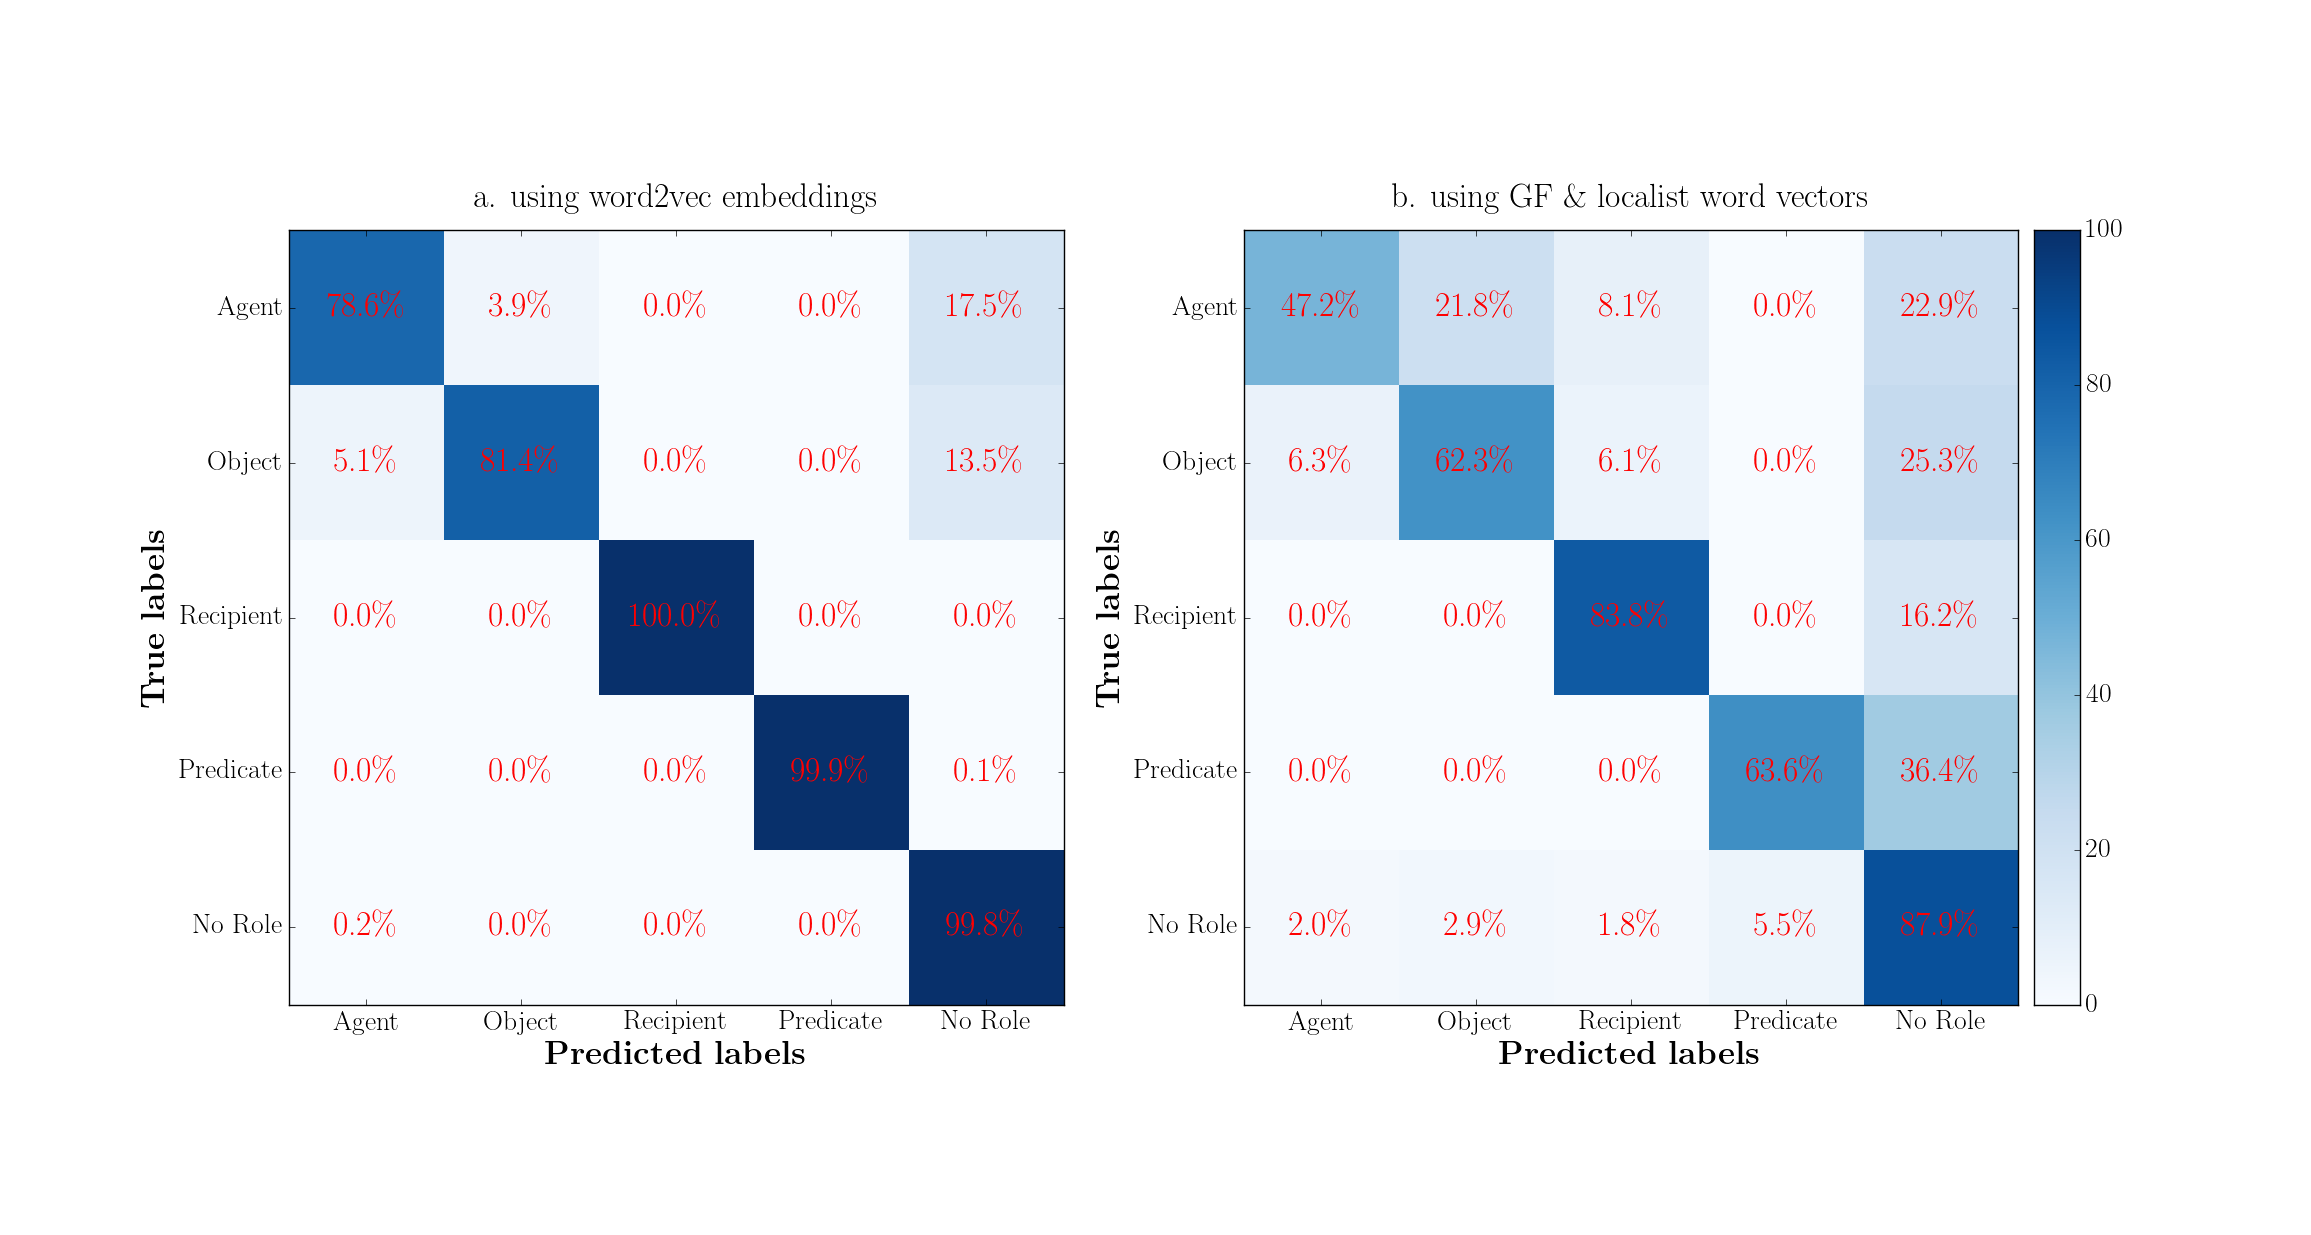
\includegraphics[width=1.0\linewidth]{confusion_matrix}
\caption[Normalized confusion matrix for unscrambled corpus-462.] {\textbf{Normalized confusion matrix with Word2Vec-ESN classifier in configuration-1 and configuration-2:}{\small The confusion matrix with true roles (in rows) and predicted roles (in columns). The top-left to bottom-right diagonal shows the percentage of words whose roles are predicted correctly. Everything other than this diagonal represents the incorrect prediction of roles. Configuration-1: raw sentences processed by Word2Vec-ESN classifier and word2vec word vectors are input to ESN. Configuration-2: Sentences transformed to grammatical form and localist word vectors are input to ESN. The results were obtained with reservoir of 1000 neurons and 10-fold cross-validation.}}
\label{fig:confusion_matrix}
\end{figure}

% CONFUSION MATRIX SCRAMBLED
\begin{figure}[hbtp]
\centering
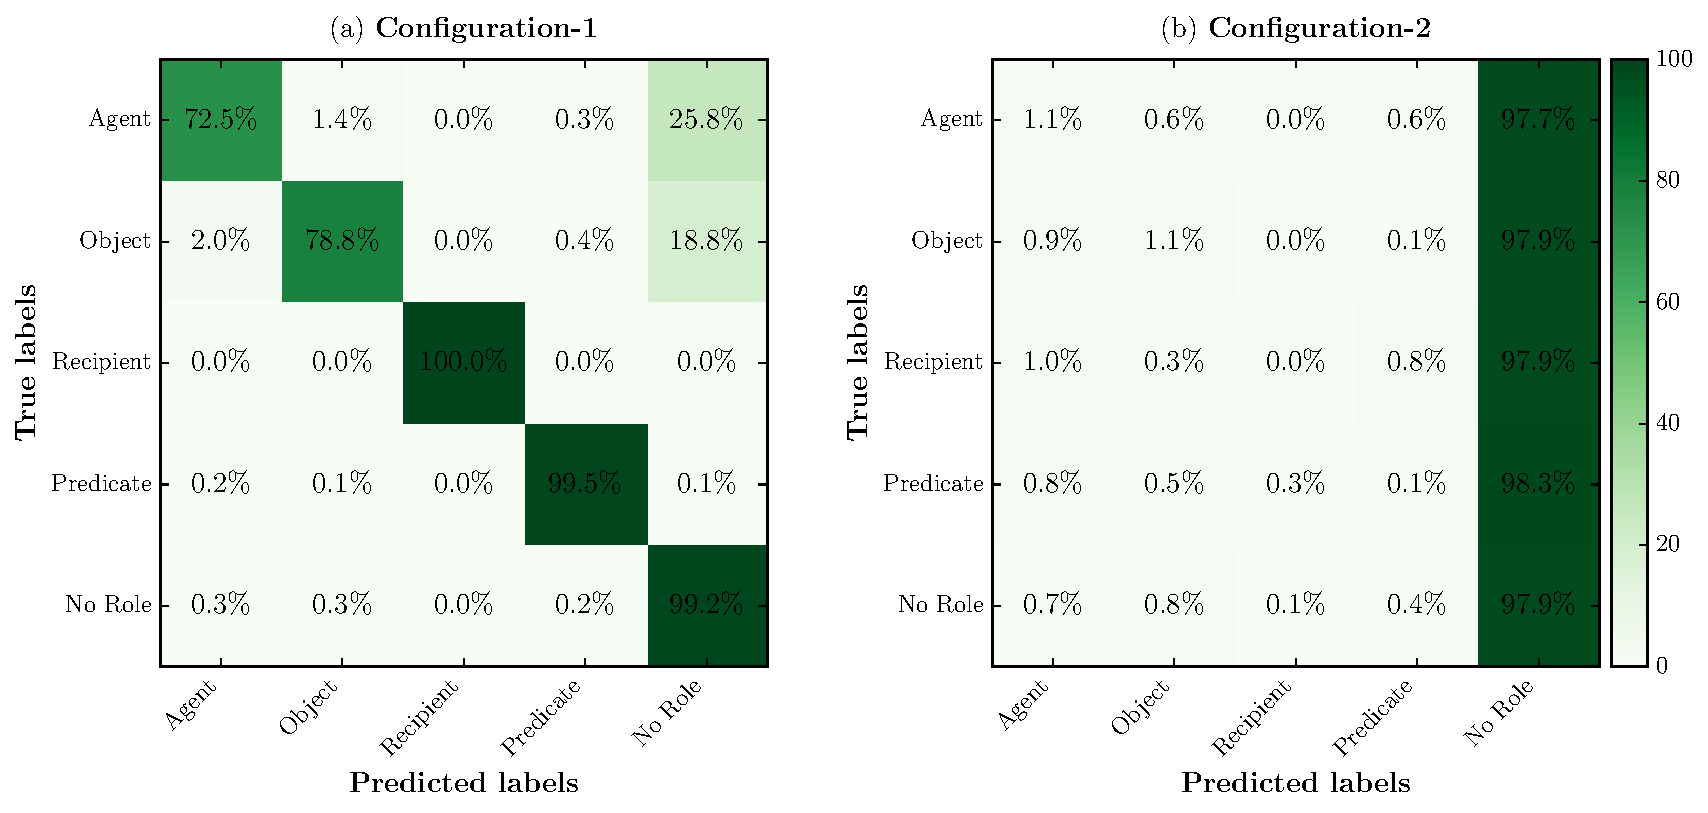
\includegraphics[width=1.0\linewidth]{confusion_matrix_shuffle}
\caption[Normalized confusion matrix for scrambled corpus-462.] {\textbf{Normalized confusion matrix with the Word2Vec-ESN classifier on scrambled corpus-462: } {\small The confusion matrix shows the true roles (in rows) and predicted roles (in columns) of argument-predicate pairs. The top-left to bottom-right diagonal shows the percentage of argument-predicate pairs for which the roles are predicted correctly. All cells, other than this diagonal represents the incorrect prediction of the roles. Configuration-1: raw sentences processed by the Word2Vec-ESN classifier and distributed word vectors are input to ESN. Configuration-2: Sentences transformed to grammatical form and localist word vectors are input to ESN. The results were obtained with reservoir of 1000 neurons.}}
\label{fig:confusion_matrix_shuffle}
\end{figure}

Figure \ref{fig:confusion_matrix} shows the confusion matrices of true and predicted roles for input argument-predicate pairs in confguration-1 and configuration-2. The matrices are plotted using the cross-validation results of the Word2Vec-ESN classifier. The corresponding classification scores of the individual roles produced by the classifier during 10-fold cross-validation are also reported in Table \ref{tab:classsification-scores-21} for both the configurations.

As shown in the confusion matrix (see fig. \ref{fig:confusion_matrix}), it can be observed that when using the distributed vectors of argument-predicate pair as an input to ESN (i.e. configuration-1), the model predicted the roles `Recipient', `Predicate' and `No Roles' almost without making any errors. Notice that the classifier mispredicted the roles `Agent' and `Object' mostly as `No Role'. It can also be noticed that the roles `Agent' and `Object' were confused with each other i.e. the argument-predicate pairs with the role `Agent' were misclassified as `Object' and vice-versa. 

Using the sentences in grammatical form along with the localist word vectors of the argument-predicate pairs (i.e. configuration-2), as an input to ESN, the roles `Recipient' and `No Role' were predicted correctly with least errors of $16.2 \%$ and $12.1 \%$. Notice that significant amount of all the roles were misclassified as `No Role', where the `Predicate' being the highest role to be misclassified ($36.4 \%$) as `No Role'. The classifier in configuration-2 also seems to be confused between the roles `Agent' and `Object'. Additionally, the argument-predicate pairs with the true roles `Agent' and `Object' were also confused with the role `Recipient'. 

While comparing the predictions made by the Word2Vec-ESN classifier in both the configurations, it was observed that the roles `Agent' and `Object' made the most number of errors in predictions as compared to other roles. In both the configurations, the model was mainly confused between roles `Agent' and `Object', but with the higher number of misclassification in configuration-2. Additionally, in configuration-2, the roles `Agent' and `Object' were wrongly predicted as `Recipient', whereas in configuration-1, this misprediction does not exist. Comparing the false predictions made by the classifier in both the configurations, it can be observed that the number of incorrect predictions was comparatively less in configuration-1. Also, in configuration-1, all the argument-predicate pairs with actual roles `Recipient', `Predicate' and `No Role' were predicted almost without any errors whereas, in configuration-2, the classifier misclassified these roles respectively by $16.2 \%$, $36.4\%$, and $12.1 \%$.


%NOTE: 08/09/2016 results are copied after the simulation and are final, no need to change.
\begin{table}[h]
\centering
\begin{threeparttable}
\caption{Training and testing classification scores for individual roles when using Word2Vec-ESN classifier in two different configurations.}
\label{tab:classsification-scores-21}
\rowcolors{2}{gray!25}{white}
\begin{tabularx}{\textwidth}{llYYYYYYY}
\hiderowcolors
\toprule
  &  & \multicolumn{3}{c}{Configuration-1} & \multicolumn{3}{c}{Configuration-2}& \\  
\cmidrule(lr){3-5}   \cmidrule(lr){6-8}
   
Role                 &             & Pr   & Re  & F1         & Pr  &  Re & F1         &  Support  \\
\showrowcolors
\midrule
               
\textbf{Agent}        &test         & 0.92 & 0.79 & 0.85     & 0.63 & 0.47 & 0.54    & 888  \\
                    &train      & 0.94 & 0.80 & 0.86     & 0.64 & 0.46 & 0.53    & 892  \\
\textbf{Object}        &test         & 0.95 & 0.81 & 0.88     & 0.51 & 0.62 & 0.56    & 791  \\
                    &train      & 0.96 & 0.82 & 0.88     & 0.51 & 0.61 & 0.56    & 794  \\
\textbf{Recipient}    &test         & 1.00 & 1.00 & 1.00     & 0.52 & 0.84 & 0.64    & 382  \\
                    &train      & 1.00 & 1.00 & 1.00     & 0.52 & 0.83 & 0.64    & 384  \\
\textbf{Predicate}    &test        & 1.00 & 1.00 & 1.00     & 0.51 & 0.64 & 0.57    & 888  \\
                    &train      & 1.00 & 1.00 & 1.00     & 0.51 & 0.64 & 0.57    & 892   \\
\textbf{No Role}    &test         & 0.97 & 1.00 & 0.99     & 0.92 & 0.88 & 0.90    & 9776  \\
                    &train      & 0.97 & 1.00 & 0.99     & 0.91 & 0.88 & 0.90    & 9823  \\
\bottomrule
\end{tabularx}
\begin{tablenotes}
\small
\item Training and cross-validation classification scores (precision upto 2 decimals) for each output roles predicted by the Word2Vec-ESN classifier in two configuration. Support for each role: actual number of instances, is also shown in last column. Simulation condition: 1000 reservoir neurons, 10-fold cross-validation.
\end{tablenotes}
\end{threeparttable}
\end{table}

\section{Experiment-3: Effect of Corpus Structure} 

As described earlier, the sentences in the corpus-462 were created based on context-free grammar. Thus the sentences in the corpus contain an inherent grammatical structure. The models are thus possibly utilizing the underlying grammatical structure to some extent for learning and generalization. To test this hypothesis and to demonstrate that the models are not generalizing on any other inconsistent regularity in the corpus, in this experiment, the inherent grammatical structure from the sentences of corpus-462 was removed by randomizing the word orders within the sentences \cite{xavier:2013:RT}. Such a test will also help us to have an insight on what the model is actually learning and whether the model is overfitting or not. 

For the simulations, the corpus-462 with the scrambled sentences (i.e. in the absence of any grammatical structure) was presented to the Word2Vec-$\theta$RARes model and Word2Vec-ESN classifier. Keeping all conditions and the reservoir parameters same as used in Experiment-2 for both the models, a 10-fold cross-validation was performed with five model instances. Apart from cross-validation, the models were also trained and tested on all the sentences in the corpus to determine the learning ability of the models with the scrambled corpus.

\paragraph{Word2Vec-$\theta$RARes model:}

As illustrated in Table \ref{tab:corpus-462_errors}, it was observed that when using the scrambled corpus as an input to the Word2Vec-$\theta$RARes model, the model learned the scrambled sentences with low error rates of $ME = 6.68 \%$ and $SE = 26.80 \%$ in SCL mode. While testing, the model generalized with cross-validation error rates of $ME = 70.15 \% $ and $SE = 99.26 \%$. Similarly, in SFL mode the model learned with low error rates of $ME = 9.38 \%$ and $SE = 35.58 \%$  but during cross-validation high error rates of $ME = 67.87 \%$ and $SE = 99.26 \% $ was observed. Notice that the model learned the scrambled corpus with low error rates while training, but during the cross-validation, it generalized with high error rates. While comparing the results of Word2Vec-$\theta$RARes model with and without inherent grammatical structures in the sentences, it can be observed that the model did not perform better on the corpus with the scrambled sentences. This indicates that the model is not generalizing on any other inconsistent regularity in the corpus, but instead utilizing the grammatical structure present in the sentences.


\paragraph{Word2Vec-ESN classifier:} Table \ref{tab:corpus-462-scores} illustrates the effect of the scrambled corpus on the Word2Vec-ESN classifier. It can be observed that in the configuration-1, the classification scores in training and testing conditions, remained almost equivalent to the scores obtained with the unscrambled corpus. Whereas in configuration-2, the Word2Vec-ESN classifier learned and generalized on the scrambled corpus with low classification scores. Also in configuration-2, notice the classification scores in both the training and testing conditions are lower than that obtained with the unscrambled corpus. 

Figure \ref{fig:confusion_matrix_shuffle} shows the confusion matrix obtained when the scrambled corpus is exposed to Word2Vec-ESN classifier. It was observed that in configuration-1, the Word2Vec-ESN classifier classifies the argument-predicate pair to the respective roles with high classification scores whereas, in configuration-2, it fails to do so. Comparing the confusion matrix obtained when using unscrambled corpus-462 (see fig. \ref{fig:confusion_matrix}) and scrambled corpus-462 (see fig. \ref{fig:confusion_matrix_shuffle}) it is clearly visible that in configuration-1, the classification scores for each role is negligibly affected whereas in configuration-2, the classification scores of individual roles dropped heavily.

\section{Experiment-4: Effect of Reservoir Size}

The most important hyperparameter which affects the performance of the proposed models is the size of the reservoir (i.e. $N_{x}$ = number of neurons in the reservoir). The addition of neurons in the reservoir is computationally inexpensive because the read-out weights ($W^{out}$) scales linearly with the number of neurons in the reservoir \cite{esn:learn_gs}. Liu et al. \cite{overfitting:liu} argued that as the number of neurons in the neural network increases, so does the danger of overfitting, thus ensuring the failure of the network to generalize during cross-validation. So, in order to determine the effect of reservoir size on the performance of the Word2Vec-$\theta$RARes model and Word2Vec-ESN classifier, the simulations were performed over a range of reservoir sizes \footnote[1]{Reservoir sizes explored in Word2Vec-$\theta$RARes model: [90, 291, 493, 695, 896, 1098, 1776, 2882, 3988, 5094]} \footnote[2]{Reservoir sizes explored in Word2Vec-ESN classifier: [50, 100, 250, 400, 600, 800, 1050, 1600, 2250, 3320, 3860, 4500]} with the five instances of the proposed models. The sizes of the reservoir were randomly chosen from a range of 50 to 5500 neurons. Also, for the simulations, corpus-462 was used, and models were tested using 10-fold cross-validation approach.

\paragraph{Word2Vec-$\theta$RARes model: } 

With the Word2Vec-$\theta$RARes model, simulations were performed on a range of reservoir size\footnotemark[1] in both the SCL and SFL modes, using the same optimal reservoir parameters as used in Experiment-2 i.e. $SR = 2.4$, $IS = 2.5$ and $LR = 0.07$ in SCL mode and $SR = 2.2$, $IS = 2.3$ and $LR = 0.13$ in SFL mode. 

\begin{figure}[hbtp]
\centering
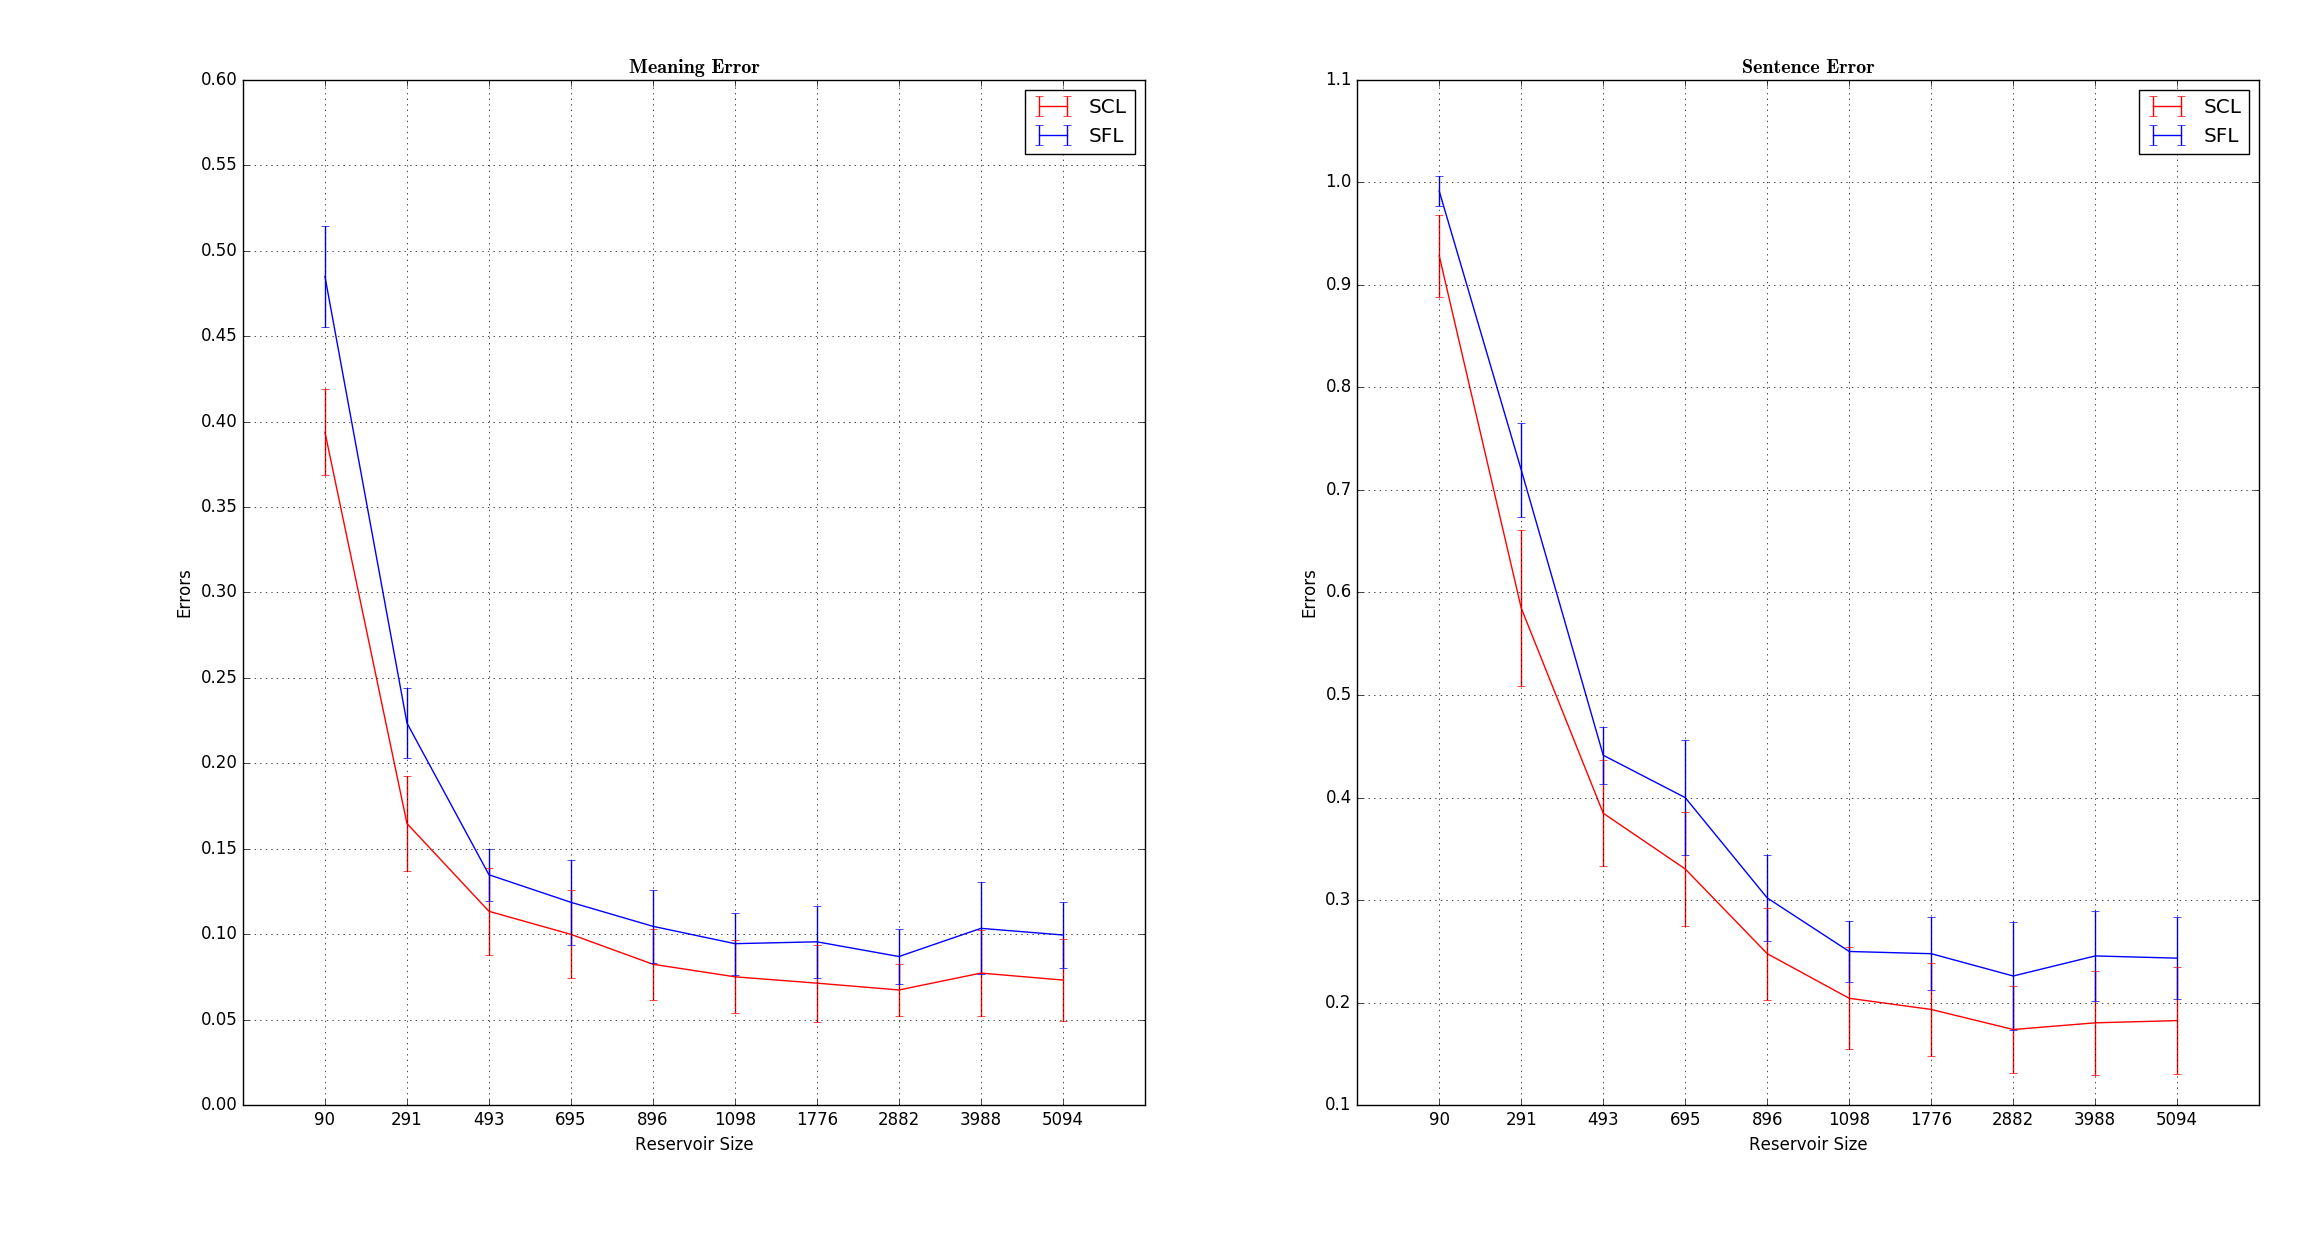
\includegraphics[width=1.0\linewidth]{reservoir_size_1}
\caption[Effect of reservoir size on Word2Vec-$\theta$RARes model.]{Effect of reservoir size on cross-validation errors of Word2Vec-$\theta$RARes model. NOTE: the scale of cross-validation error for the meaning and sentence error are different.}
\label{fig:reservoir_size_1}
\end{figure}

Figure \ref{fig:reservoir_size_1} shows the effect of reservoir size on the cross-validation errors rates (i.e. meaning and sentence error). The meaning and sentence errors continuously drop with the increase in reservoir size from 90 to 1098 in both the learning modes.  As the reservoir size is further increased from 1098, the meaning and sentence error in both the SCL and SFL mode is negligibly affected. Notice that with the increase in reservoir size, the meaning and sentence error curves follows the similar trend in both the SCL and SFL mode. Another interesting pattern to notice is that, with all the reservoir sizes studied, the meaning and sentence error in SCL mode is always lower than in SFL mode. Overall the important behavior to notice is that both the meaning and sentence cross-validation error rates reduce with the increase in the reservoir size, but asymptotes when the reservoir size is above 1000 neurons.

\paragraph{Word2Vec-ESN classifier: } 

To determine the effect of reservoir size on the Word2Vec-ESN classifier, simulations were performed on a range of reservoir sizes \footnotemark[2], in configuration-1 and configuration-2 of the classifier as described in Experiment-2. Also, for the simulations, reservoir parameters were kept identical to that used in Experiment-2.

\begin{figure}[hbtp]
\centering
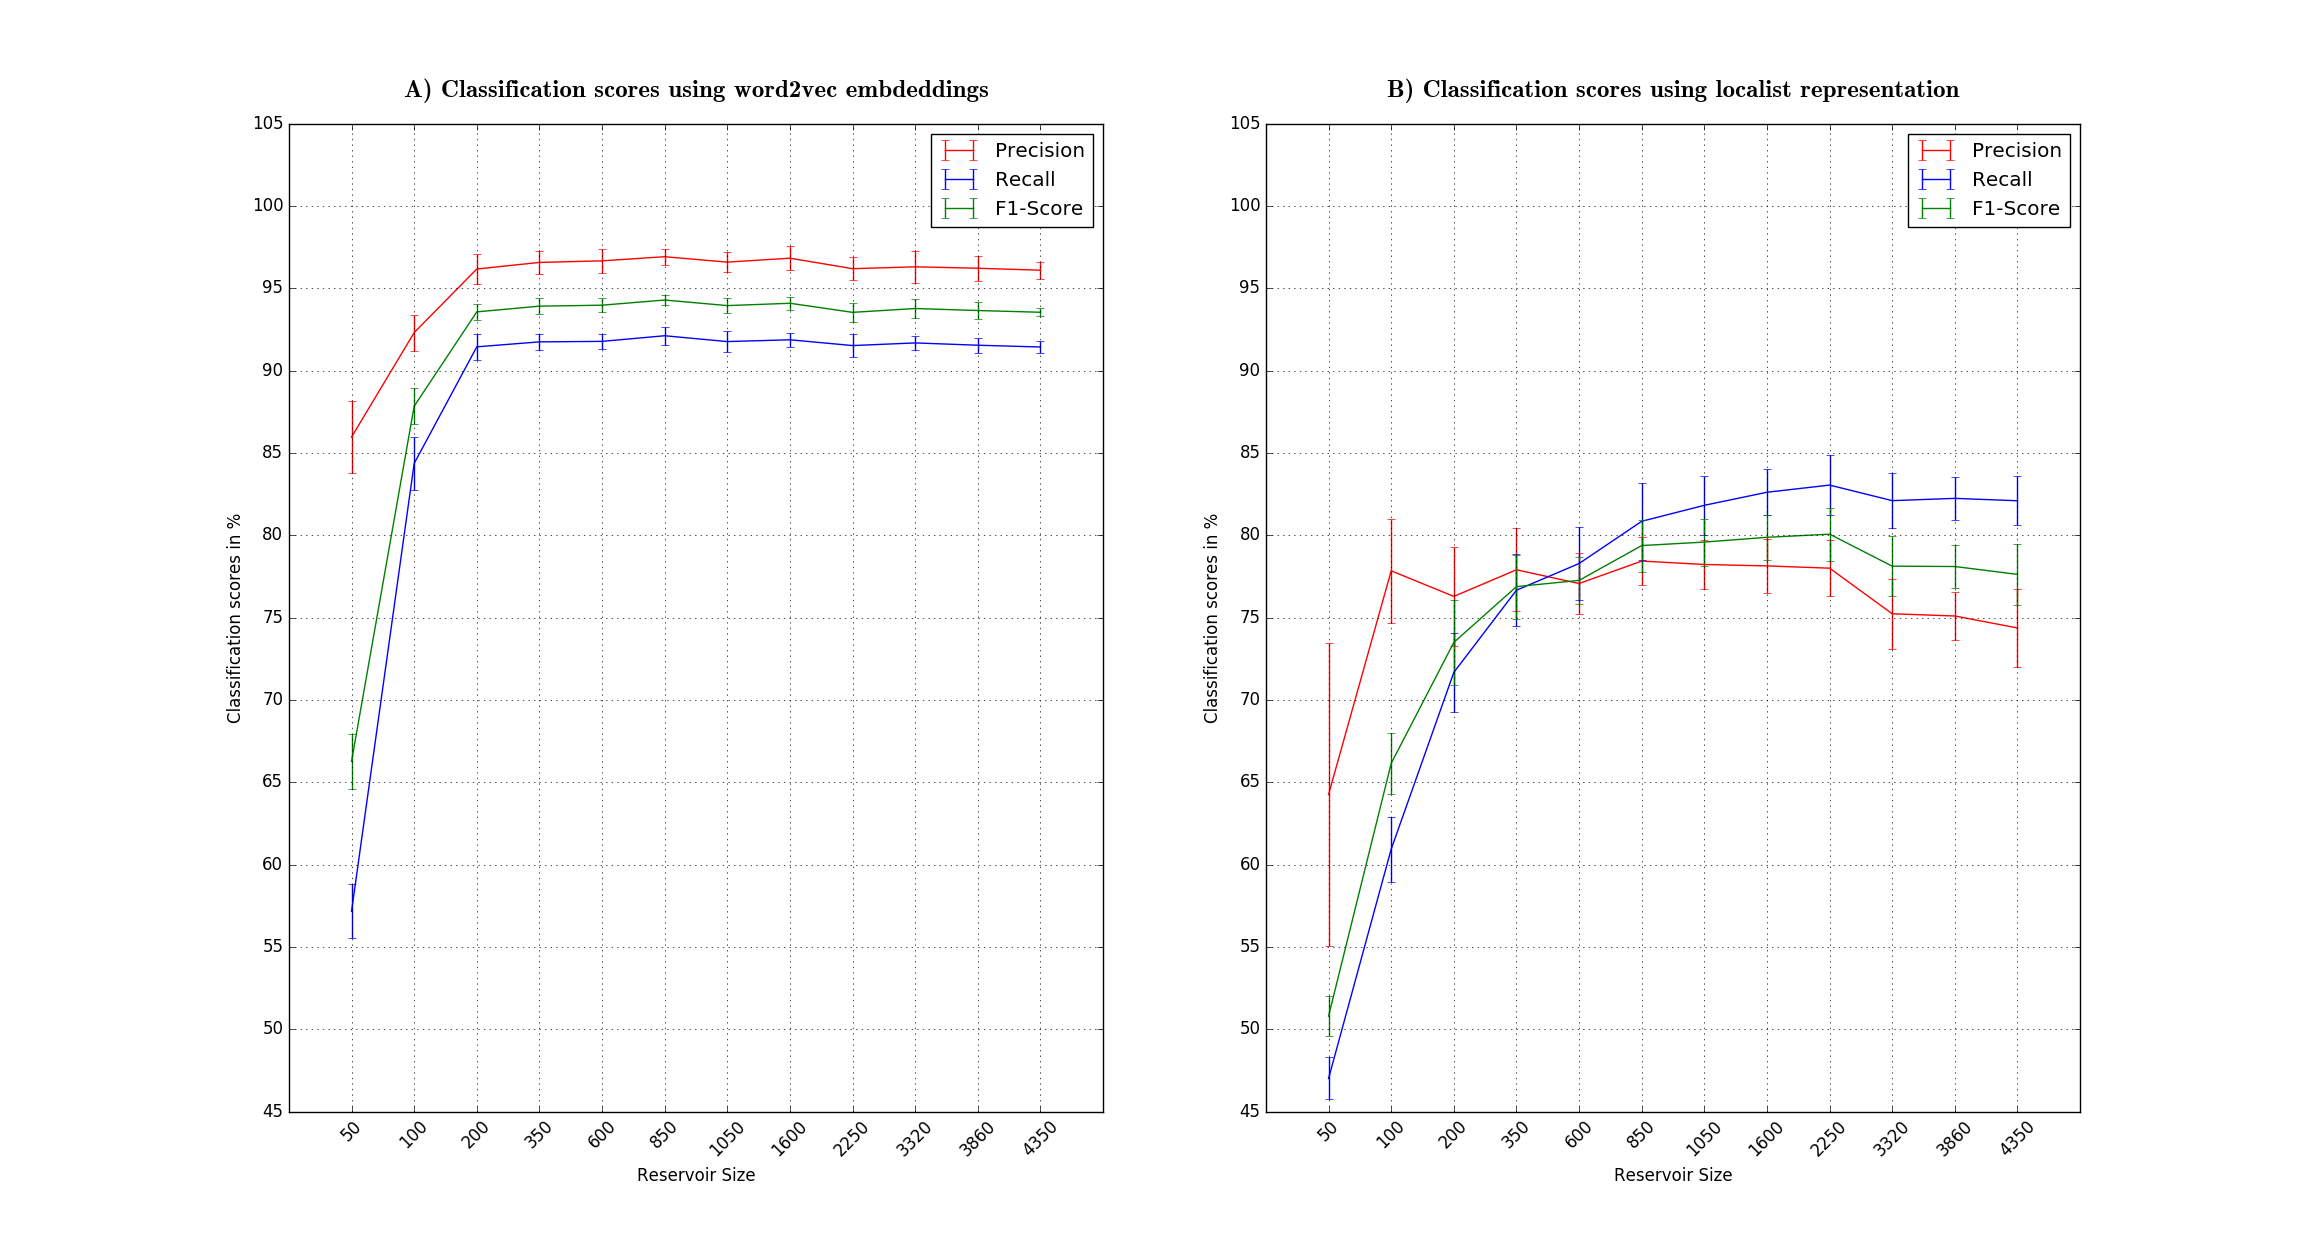
\includegraphics[width=1.0\linewidth]{reservoir_size_2}
\caption[Effect of reservoir size on Word2Vec-ESN classifier.]{Effect of reservoir size on classification scores of Word2Vec-ESN classifier. NOTE: the scale of cross-validation scores in configuration-1 and configuration-2 are different.}
\label{fig:reservoir_size_2}
\end{figure}

Figure \ref{fig:reservoir_size_2} shows the change in classification scores of the Word2Vec-ESN classifier with the increase in reservoir size. It can be observed that when using the distributed word vectors (i.e. configuration-1) the classification scores sharply increases when the reservoir size is increased from 50 neurons to 250 neurons. As the reservoir size is further increased from 250 neurons, the classification scores remain stable with the negligible drop of scores. Whereas in configuration-2 i.e. when using the sentences in grammatical form encoded using localist representation, the classification scores also improve, with the increase in reservoir size from 50 to 250 neurons. As the reservoir size is further increased from 250 neurons, the recall score is improved whereas the precision remains almost flat with negligible improvement. The F1-Score is harmonic mean of precision and recall, and thus it is also slightly increased. Notice that even the highest F1-Score of Word2Vec-ESN classifier observed at reservoir size 4500 in configuration-2 is much lower than that of observed at reservoir size 100 ($\approx 29 \%$ ) in configuration-1.

\section{Experiment-5: Scalability of the Model}

In order to investigate the effect of corpus size and to determine the scaling capability of the model, the extended corpus-90582 (see section \ref{corpora}) was used for this experiment. As this corpus also contains $12\%$ of ambiguous sentences \cite{xavier:2013:RT} which impede the learning and generalization of the model, this experiment will also validate the model's ability to process the ambiguous sentences. Thus, in order to study the scaling capability of the model with different corpus size, 6 sub-corpora were created by randomly sampling $6\%$, $12\%$, $25\%$, $50\%$, $75\%$, $100\%$ of sentences from the original corpus of 90582 sentences \cite{xavier:2013:RT}. Each of the generated sub-corpora was exposed to the Word2Vec-$\theta$RARes model, and a 2-fold cross-validation was performed. The model was trained on half the sub-corpora size and tested on remaining half. The second half used for testing was then used to train the model and tested on the first half, used for training previously. This experiment was performed with the Word2Vec-$\theta$RARes model in both learning modes i.e. SCL and SFL, using five model instances each with a reservoir of 5000 neurons. All the other reservoir parameters were kept identical to the Experiment-2.

\begin{figure}[hbtp]
\centering
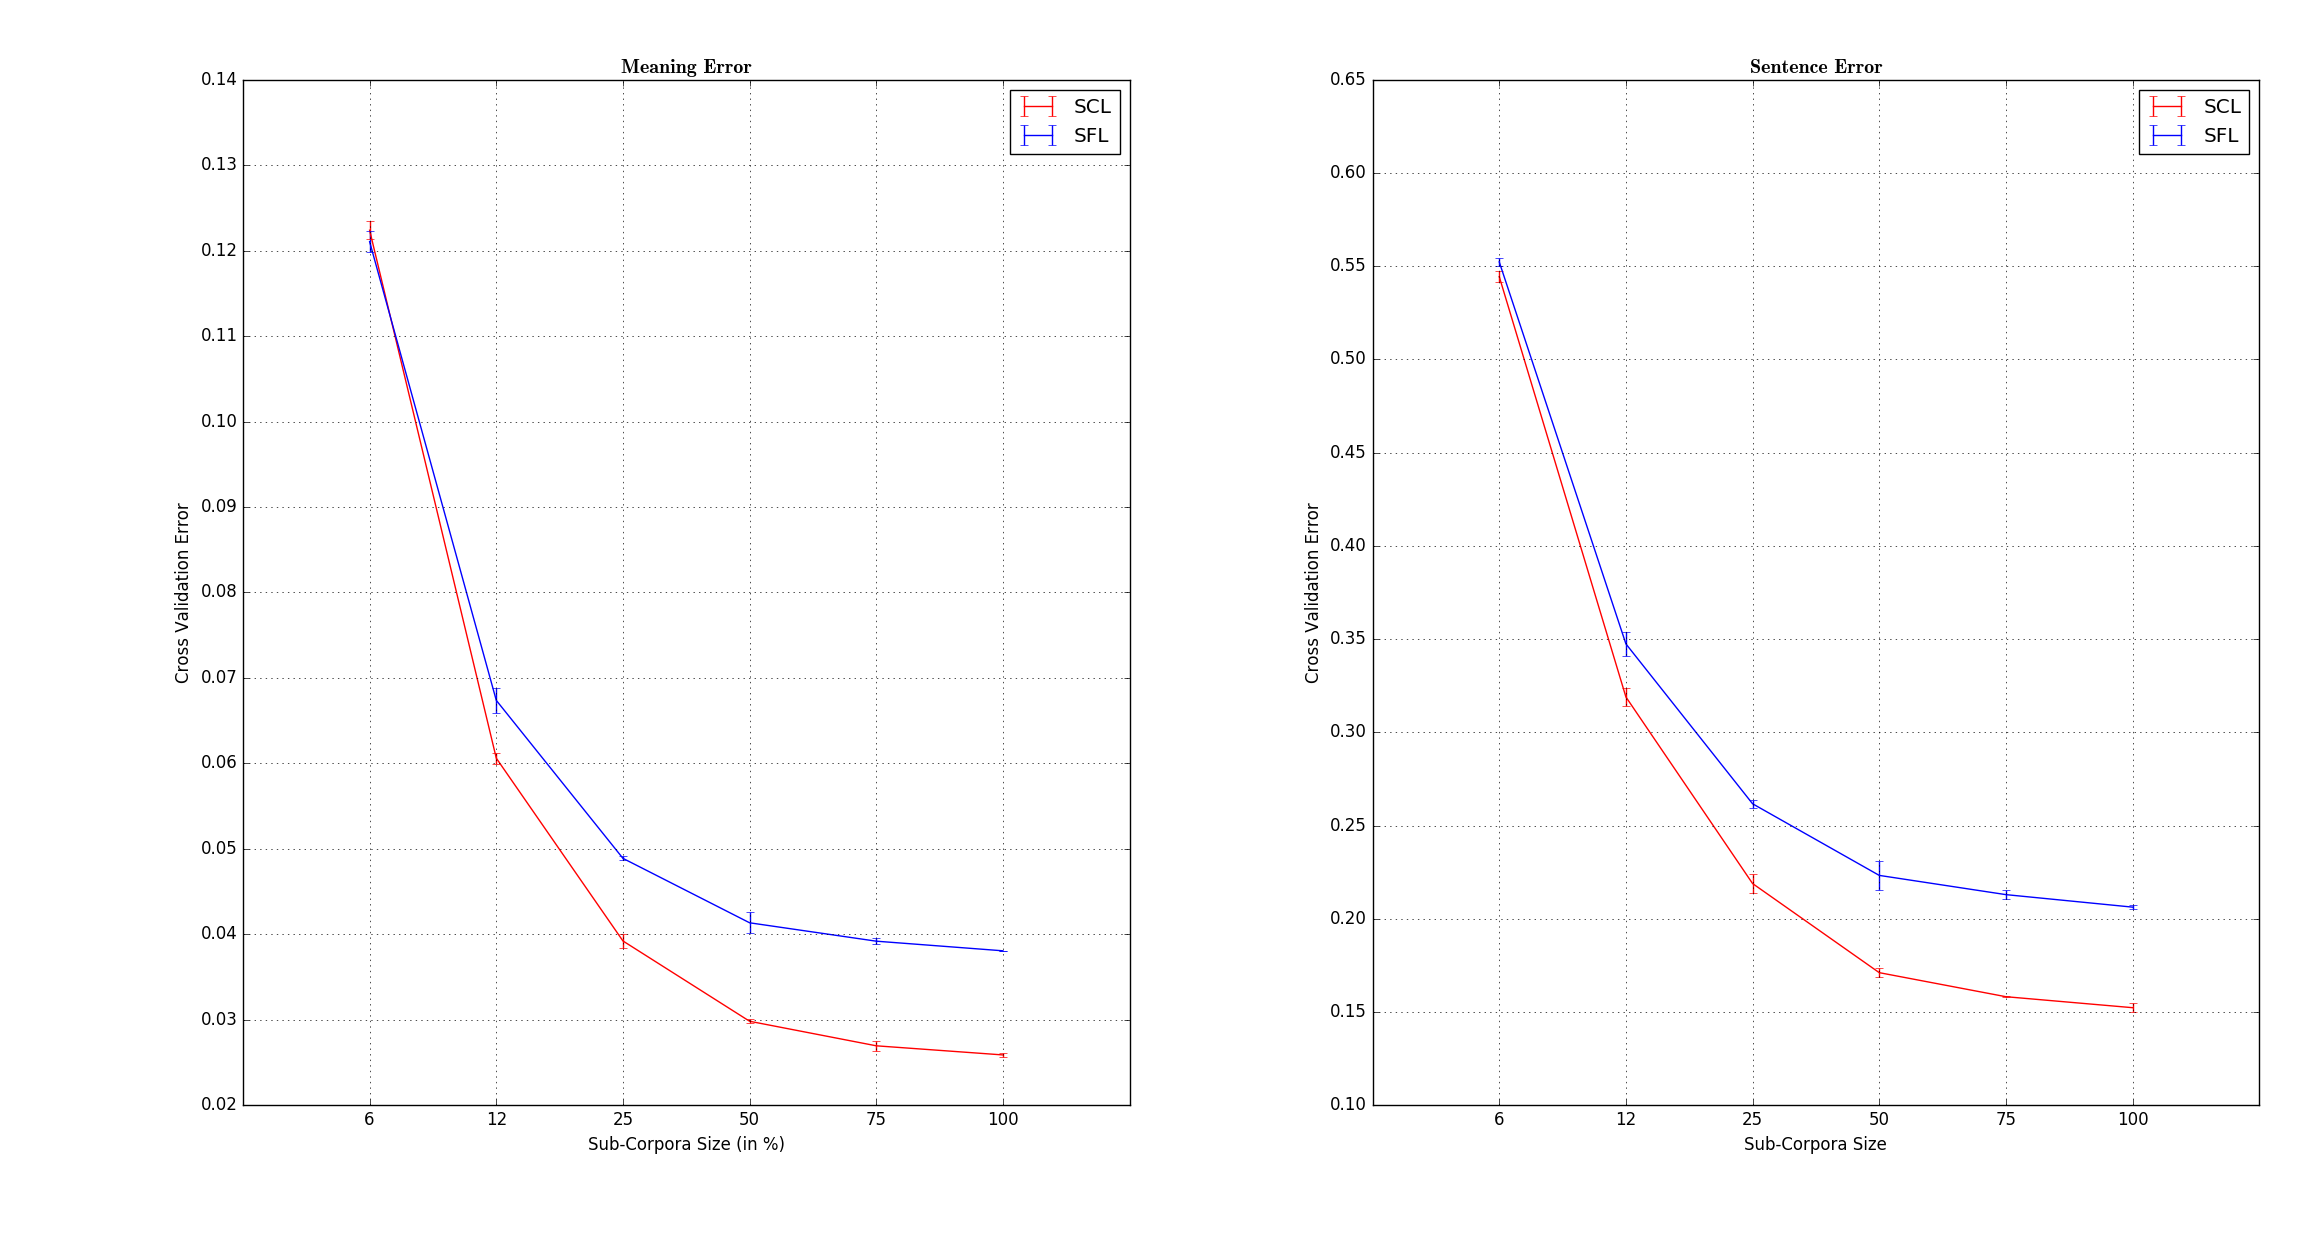
\includegraphics[width=1.0\linewidth]{corpus_size_1}
\caption[Effect of corpus size on Word2Vec-$\theta$RARes model.]{Effect of corpus size on cross validation errors of Word2Vec-$\theta$RARes model in SCL and SFL mode. NOTE: the scale of cross-validation error for the meaning and sentence error are different.}
\label{fig:corpus_size_1}
\end{figure}

Figure \ref{fig:corpus_size_1} shows the cross-validation errors rates with respect to corpus size on the Word2Vec-$\theta$RARes model. It can be observed that with the increase in corpus size from $6 \%$  to $50 \%$, the meaning error sharply drops from $12.18 \%$ to $2.96 \%$ in the SCL mode and from $11.96\%$ to $4.17 \%$ in the SFL mode. Similarly, the sentence error also decreases from $54.84 \%$ to $17.25 \%$ in SCL and from $54.14 \%$ to $22.41 \%$ in the SFL mode. When the sub-corpora size is $75\%$, where the model was trained only on $37.5\%$ of corpora size, the model already generalized with $2.72 \%$ meaning error and $15.98 \%$ sentence error in the SCL mode and with $3.95 \%$ meaning error and $21.33 \%$ sentence error in the SFL mode. Although the error rates gradually drop when the corpus size is further increased from $25\%$ to $100\%$ but the improvement rate of errors is very less. This indicates that cross-validation errors improve with the increase in corpus size up to a certain limit and any further increase in corpus size barely influence the performance of the model.

\begin{figure}[hbtp]
\centering
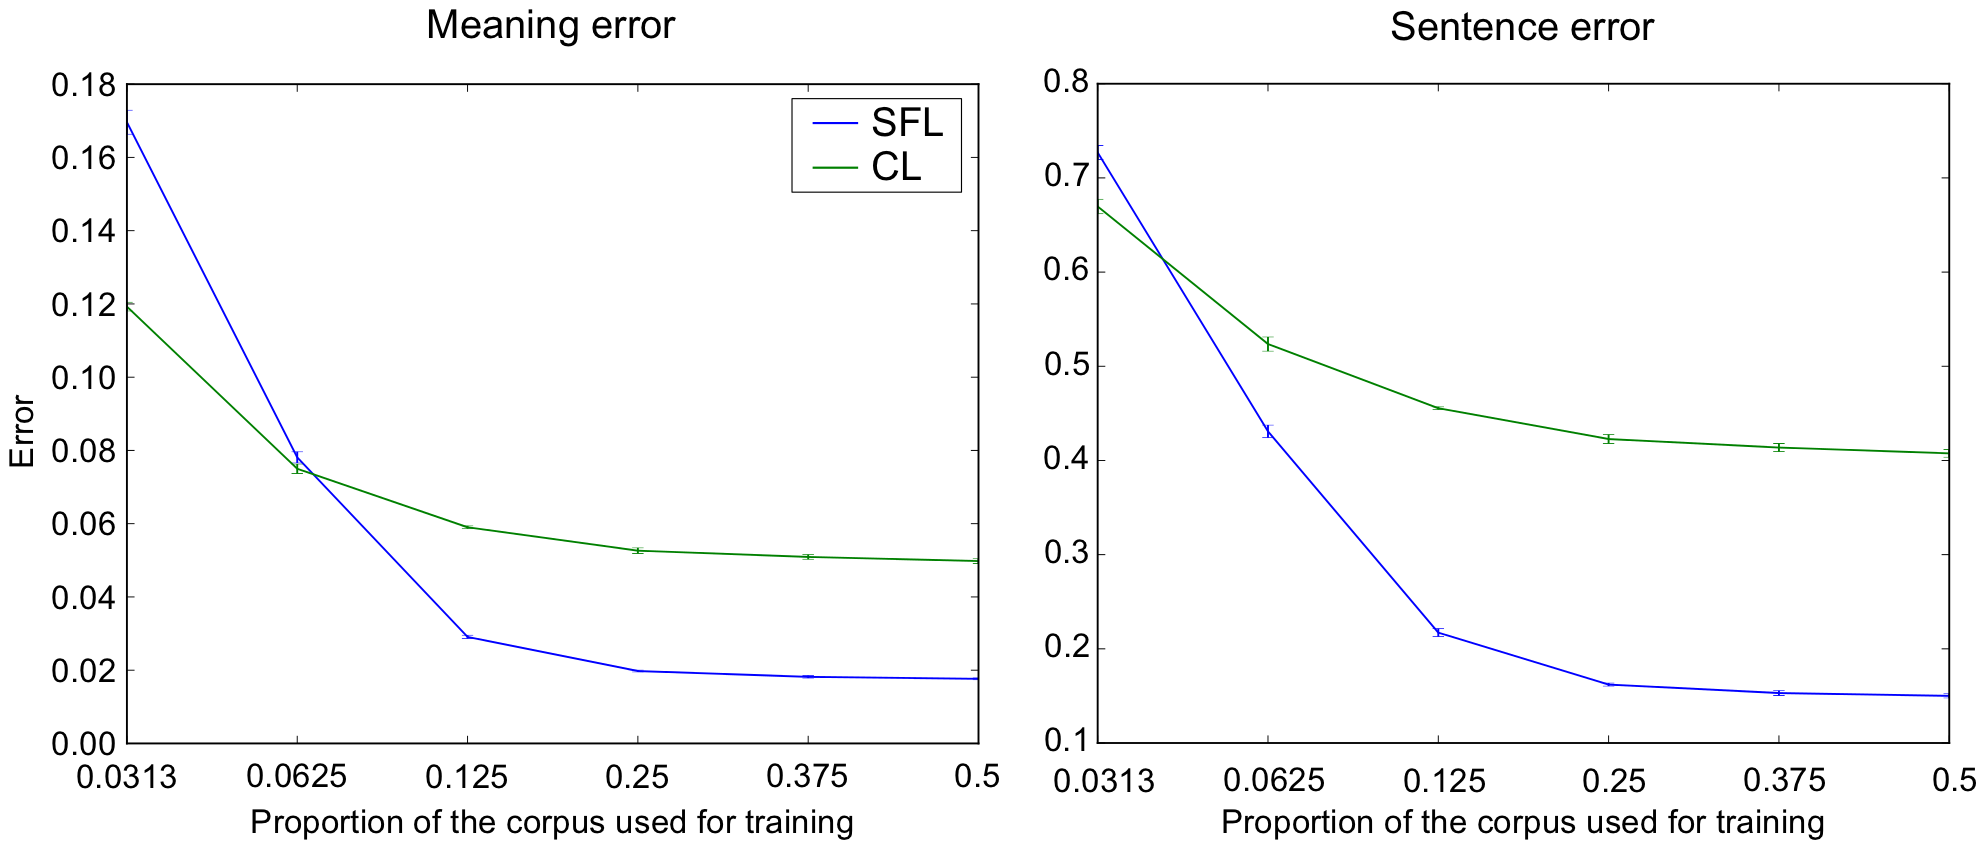
\includegraphics[width=1.0\linewidth]{corpus_size_xavier}
\caption[Effect of corpous size on $\theta$RARes model.]{Effect of corpus size on cross validation errors using $\theta$RARes model in SCL (legend CL) and SFL learning modes \cite{xavier:2013:RT}. NOTE: The x-axis represents the corpus-size used for training i.e. if sub-corpora size is $25\%$ then corresponding tick on the axis is 0.125 ($12.5\%$). The scale of cross-validation error for the meaning and sentence error are different.}
\label{fig:corpus_size_xavier}
\end{figure}

Comparing the effect of corpus size on Word2Vec-$\theta$RARes model (see fig. \ref{fig:corpus_size_1}) and the $\theta$RARes model (see fig. \ref{fig:corpus_size_xavier}), it can be observed that in SFL mode, with the increase in corpus size from $6\%$ to $25\%$, the meaning error in $\theta$RARes model dropped from $\approx 17\%$ to $\approx 3\%$ and the sentence error dropped from $\approx 70\%$ to $\approx 20\%$. Whereas in the Word2Vec-$\theta$RARes model, the meaning error dropped from $\approx 12\%$ to $\approx 5\%$ and the sentence error dropped from $\approx 55\%$ to $\approx 26\%$. Also, with the increase in corpus size further from $25 \%$, the cross-validation errors asymptotes in both the models with negligible improvement in error rates. Overall, with the increase in corpus size, the improvement in error rates with $\theta$RARes model in the SFL mode is higher as compared to Word2Vec-$\theta$RARes model.

Comparing the performance of both the $\theta$RARes and Word2Vec-$\theta$RARes model in the SCL mode, it can be seen that the meaning error in latter continuously drops when the corpus size is further increased from $12 \%$ whereas in the $\theta$RARes model the decline in meaning error is negligible. The sentence error in $\theta$RARes model drops by a small amount when corpus size is increased from $6 \% $ to $25 \%$, but asymptotes as the corpus size is further increased from $25\%$ whereas, it gradually drops in Word2Vec-$\theta$RARes model. From the lower to the upper limit of corpus size studied, the sentence error with the  $\theta$RARes model in SCL mode dropped from $\approx 65\%$ to $\approx 40\%$ whereas, in the Word2Vec-$\theta$RARes model it dropped from $\approx 55\%$ to $\approx 15 \% $. The meaning error in SCL mode, on the other hand, dropped from $\approx 12\%$ to $\approx 5\%$ in the $\theta$RARes model whereas, in the Word2Vec-$\theta$RARes model it dropped from $\approx 12\%$ to $\approx 2\%$.

Overall, in SCL mode, it can be seen that on the range of sub-corpora size investigated in the experiment, the Word2Vec-$\theta$RARes model performed better than $\theta$RARes model with all sub-corpora sizes. Whereas in SFL mode, the $\theta$RARes model performs better than Word2Vec-$\theta$RARes model. Another pattern which can be observed is that with all sub-corpora sizes, the Word2Vec-$\theta$RARes model performs better in the SCL mode than the SFL mode. Whereas in the $\theta$RARes model, with the increase in corpus size the model performs better in SFL model than SCL mode. 

\section{Experiment-6: Generalization on New Corpus}

One may argue that the previously used corpora (corpus-462 and corpus-90582), were artificially constructed using context-free grammar and may add a bias to the model, thus making it easier for the model to learn and generalize on these corpora for the TRA task. To answer this question, in this experiment, the corpus-373 containing the instructions collected from human participants in a Human-Robot Interaction (HRI) study of language acquisition (as discussed in section \ref{corpora}) was used.

\paragraph{Word2Vec-$\theta$RARes model:} To test the generalization of Word2Vec-$\theta$RARes model on corpus-373, the model was operated in SCL mode and tested using the LoO cross-validation method. The SCL mode and the LoO method were chosen so that the results of this experiment can be compared with that of obtained using $\theta$RARes model \cite{tra:xavier_hri}. Also, to make the results of both the model deterministically comparable, topologically modified coding was not utilized for this experiment (see section \ref{sec:w2v-esn_model}) and simulations were performed using ten reservoir instances. For this experiment, reservoir parameter space was not explored to identify the optimal reservoir parameters, instead, the previously optimized parameters obtained on corpus-462 with topological modified coded meaning was used i.e. $SR = 2.4$, $IS = 2.5$ and $LR = 0.07$ (see section \ref{grid_search}). Doing so will also enable us to test the robustness of these model parameters on the new corpus i.e. corpus-373.

Table \ref{tab:corpus_373} reports the mean sentence error and best generalization error values obtained with the Word2Vec-$\theta$RARes and $\theta$RARes model. The best generalization error here represents the percentage of sentences whose meanings were predicted incorrectly in common by all 10 model instances \cite{tra:xavier_hri}. In comparison to the $\theta$RARes model, the mean sentence error in the Word2Vec-$\theta$RARes model improved by $26.31\%$ and $17.97\%$  with the reservoir of size 500 and 1000 respectively. The best generalization errors also improved by $17.96 \%$ and $9.12 \%$ with the reservoir size 500 and 1000 respectively.

The Word2Vec-$\theta$RARes model generalized better with both the reservoir sizes (500 and 1000) as compared to the $\theta$RARes model. Notice the improvement in both the models with the increase in reservoir size from 500 to 1000 neurons. It can be seen that the improvement in cross-validation error in the Word2Vec-$\theta$RARes model is comparatively less than the $\theta$RARes model. With the increase in reservoir size from 500 to 1000, the mean sentence error and the best generalization error in $\theta$RARes improved by $10.7 \%$ and $9.65 \%$ respectively. Whereas with the Word2Vec-$\theta$RARes model, the mean sentence error and the best generalization error improved by $2.36 \%$ and $0.81\%$ respectively. This suggests that the generalization ability of the Word2Vec-$\theta$RARes model on corpus-373 is negligibly affected by the increase in reservoir size.  

\begin{table}
\centering
\begin{threeparttable}
\caption[Word2Vec-$\theta$RARes model generalizing on new corpus]{Generalization error in SCL mode on corpus-373.}
\label{tab:corpus_373}
\rowcolors{2}{gray!25}{white}
\begin{tabular}{llcc}
\hiderowcolors
\toprule
Reservoir              &  Error     &   Word2Vec-$\theta$RARes Model        & $\theta$RARes Model \\
\midrule
\showrowcolors                 
\textbf{500 N}    & mean (std.)         & 42.65 ($\pm$ 1.36)     & 68.96 ($\pm$ 2.03)  \\
                    & Best             & 26.54                 & 44.50  \\
\textbf{1000 N}    & mean (std.)         & 40.29 ($\pm$ 1.13)     & 58.26 ($\pm$ 1.37)\\
                    & Best             & 25.73                 & 34.85 \\
\bottomrule
\end{tabular}
\begin{tablenotes}
\small
\item 
Sentence and best generalization errors (in $\%$) obtained with the Word2Vec-$\theta$RARes model and the $\theta$RARes in SCL mode with reservoir of 500 and 1000 neurons. The results reported are mean and standard deviation of errors obtained with 10 model instances. The best generalization error here means the percentage of sentences predicted incorrectly in common by all 10 reservoir instances \cite{tra:xavier_hri}.
\end{tablenotes}
\end{threeparttable}
\end{table} 

Figure \ref{fig:373_stats_500} and \ref{fig:373_stats_1000} shows the number of erroneous sentences by number of model instances with reservoir size 500 and 1000 respectively. With a reservoir of 500 neurons (see fig. \ref{fig:373_stats_500}), all the ten instances of Word2Vec-$\theta$RARes and $\theta$RARes model correctly predicted the meaning of 146 and 35 sentences respectively. Whereas the meaning of 99 and 166 sentences out of 373 was wrongly predicted by all the ten instances of Word2Vec-$\theta$RARes and $\theta$RARes model. 

\begin{figure}[hbtp]
\centering
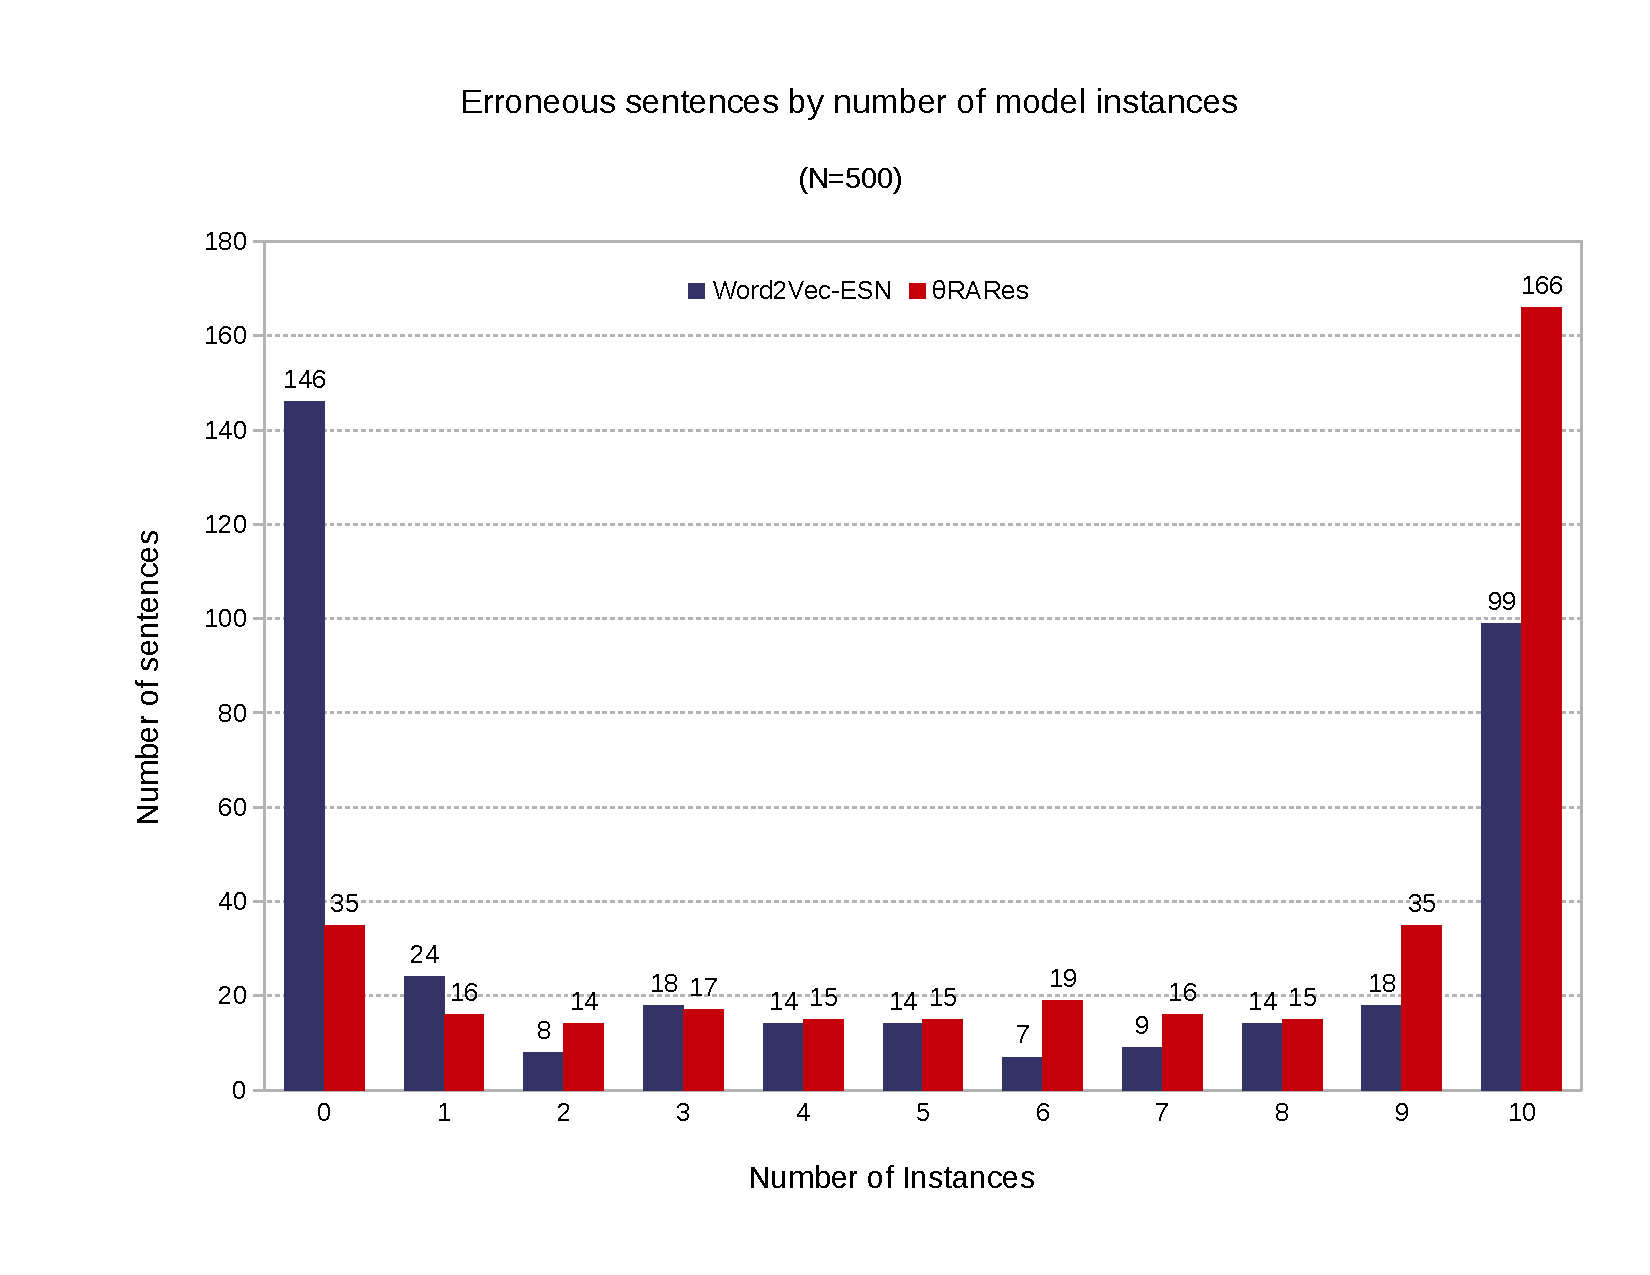
\includegraphics[width=0.9\linewidth]{500_res}
\caption[Sentence error count by number of model instances with reservoir size 500.]{Sentence error count by number of instances with reservoir of 500 neurons.}
\label{fig:373_stats_500}
\end{figure}

\begin{figure}[hbtp]
\centering
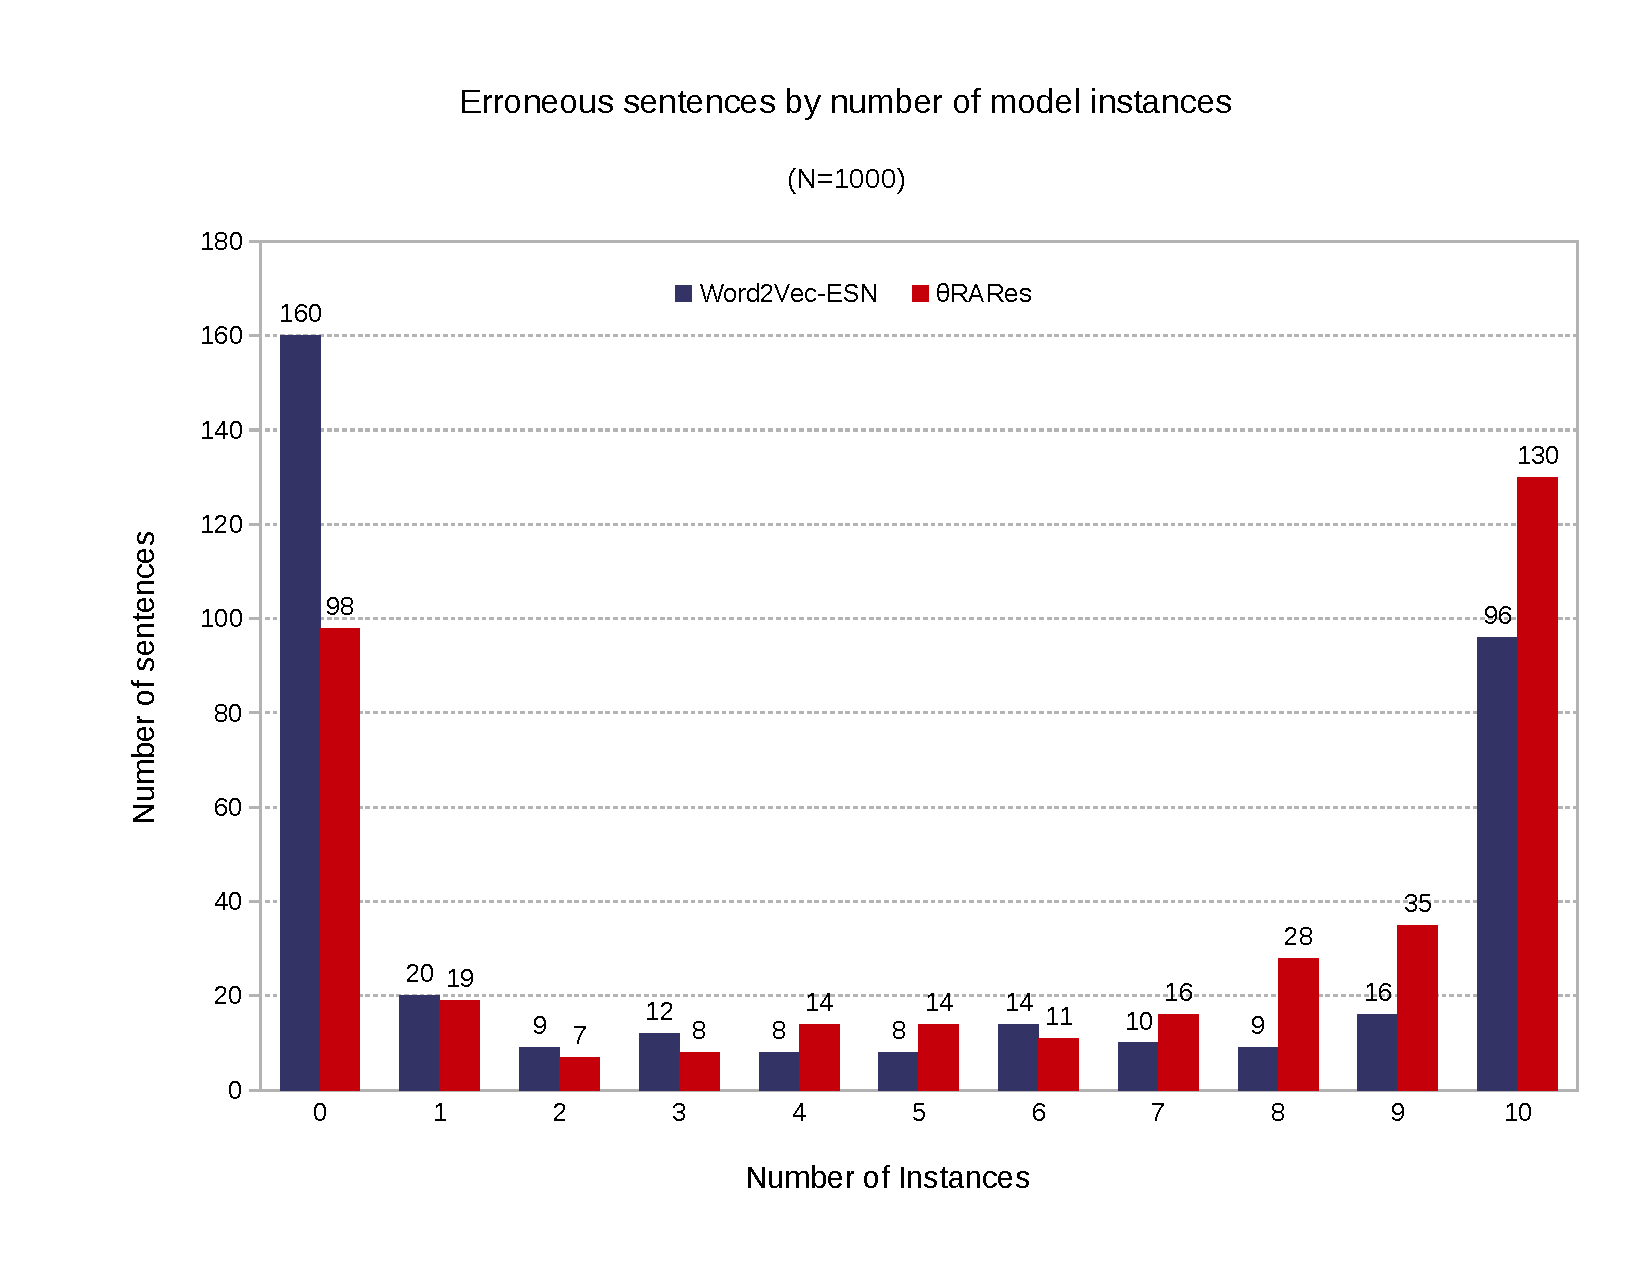
\includegraphics[width=0.9\linewidth]{1000_res}
\caption[Sentence error count by number of model instances with reservoir size 1000.]{Sentence error count by number of model instances with reservoir of 1000 neurons.}
\label{fig:373_stats_1000}
\end{figure}

With the increase in the reservoir from 500 to 1000 neurons, the number of sentences correctly predicted by all the instances of Word2Vec-$\theta$RARes and $\theta$RARes model increased respectively from 146 to 160 and from 35 to 98. Also, the count of sentences where all model instances failed to predict the meaning correctly dropped from 99 to 96 and 166 to 130 for Word2Vec-$\theta$RARes model and $\theta$RARes model respectively. Notice that with both the reservoir sizes, the number of sentences whose meanings were correctly predicted by all the model instances of Word2Vec-$\theta$RARes model is higher than the $\theta$RARes model. Whereas the count of sentences wrongly predicted by all model instances is lower in Word2Vec-$\theta$RARes model as compared to that of $\theta$RARes model.

\section{Experiment-7: Effect of Word2Vec Word Dimensions}

In all the previous experiments, the distributed word vectors of 50 dimensions were used. However, Mikolov et al. \cite{w2v:mikolov_2013_efficient, w2v:mikolov_2013_distributed} showed that the word vectors of higher dimensions (e.g. 300 in their case) perform better on word analogy task. Thus in this experiment, the effect of distributed word vector dimensions on the TRA task will be explored.

\paragraph{Word2Vec-$\theta$RARes model:} Recall that in section \ref{get_word_embeddings}, six Word2Vec models were trained to generate the word vectors of 20, 30, 50, 100, 200, 300 dimensions respectively. To test the effect of these word vector dimensions on the TRA task, each of these Word2Vec models was used with the Word2Vec-$\theta$RARes model. For this experiment, the sentences of corpus-373 without the topologically modified coded meaning were used (see fig. \ref{fig:model_variant_1}). Simulations were performed using ten model instances each with a reservoir of 1000 neurons. The model was trained and tested using LoO cross-validation approach in both the SCL and SFL mode, and all the reservoir parameters were kept identical to Experiment-2.

\begin{figure}[hbtp]
\centering
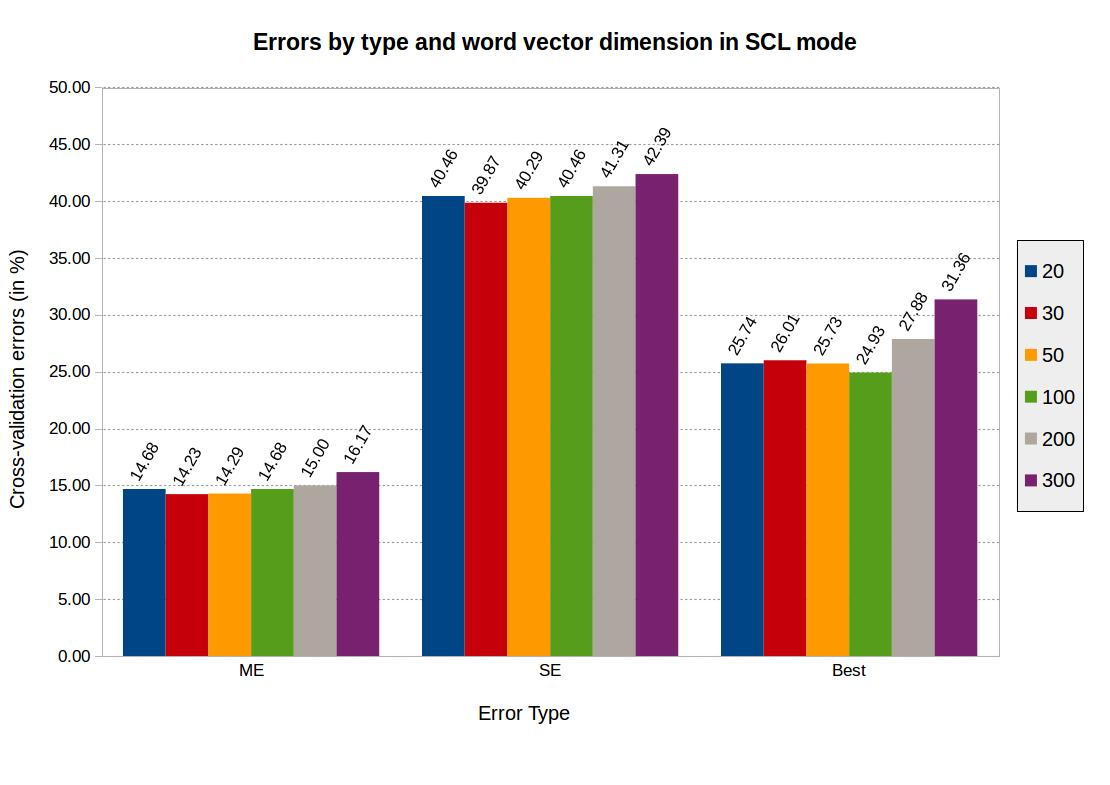
\includegraphics[width=0.9\linewidth]{word_dim_scl}
\caption[Effect of word vector dimensions on Word2Vec-$\theta$RARes model in SCL mode.]{\textbf{Effect of word vector dimensions on cross validation errors of Word2Vec-$\theta$RARes model in SCL mode: } {\small Cross-validation error are given in percentage. Error type includes ME: Meaning Error, SE: Sentence error, Best: Best generalization error.}}
\label{fig:word_dim_scl}
\end{figure}

\begin{figure}[hbtp]
\centering
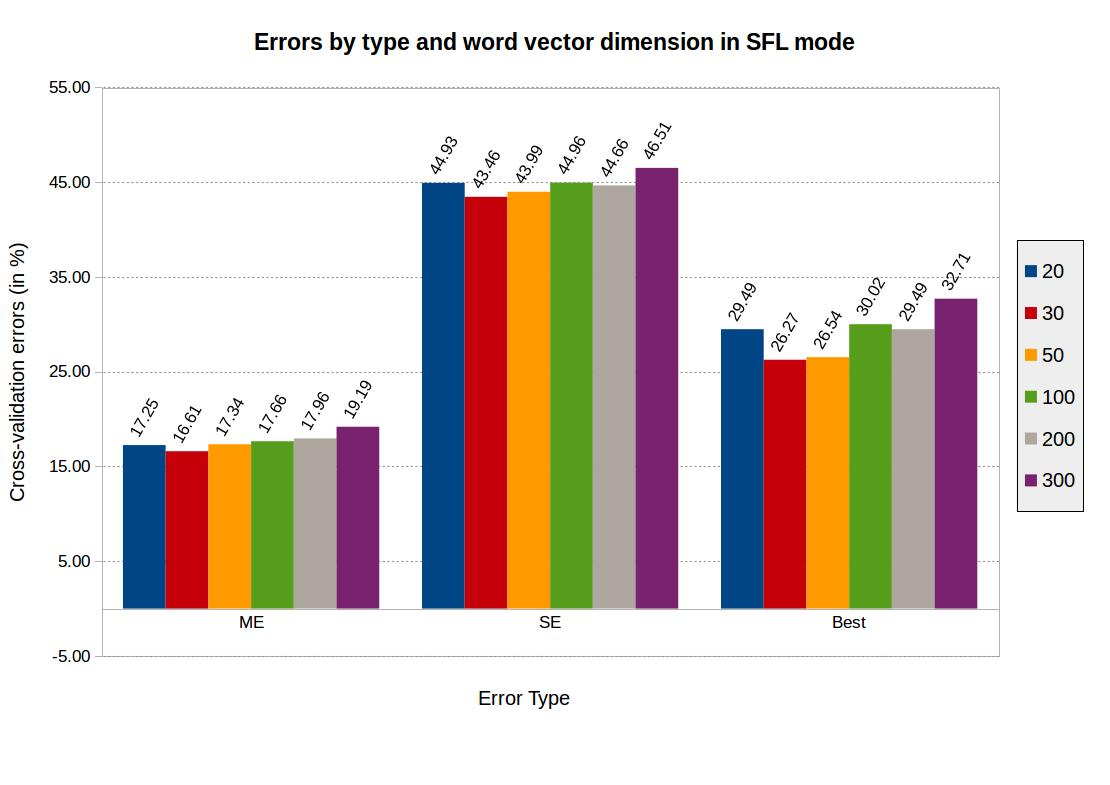
\includegraphics[width=0.9\linewidth]{word_dim_sfl}
\caption[Effect of word vector dimensions on Word2Vec-$\theta$RARes model in SFL mode.]{\textbf{Effect of word vector dimensions on cross validation errors of Word2Vec-$\theta$RARes model in SFL mode: }{\small Cross-validation errors are given in percentage. Error type includes ME: Meaning Error, SE: Sentence error, Best: Best generalization error.}}
\label{fig:word_dim_sfl}
\end{figure}

Figure \ref{fig:word_dim_scl} and \ref{fig:word_dim_sfl} shows the effect of word vector dimensions on the cross-validation errors of Word2Vec-$\theta$RARes model in SCL and SFL mode respectively. The corresponding errors are also reported in Table \ref{tab:word-vector-size}. In the figures, we can see that from lower to the upper limit of the word vector dimensions studied, all the error measures in both the learning modes increased approximately by $2\%$. Also, in the range of 20 to 200 dimensions, the cross-validation errors remained almost equivalent with negligible fluctuations. The minimum errors were obtained with word vectors of 30 dimensions i.e. $ME= 14.23$, $SE= 39.87$ in the SCL mode and $ME= 16.61$, $SE= 43.46$ in the SFL mode. Another interesting pattern which can be observed is that with all the word vector dimensions, the model in SCL mode always performed better as compared to SFL mode. The similar relation between SCL and SFL mode was also observed in the previous experiments as well. Overall, it was observed that the word vectors dimensions have a negligible effect on the performance of Word2Vec-$\theta$RARes model for the TRA task.

\section{Neural Output Activity of the Word2Vec-$\theta$RARes Model}

In the previous experiments, we observed that the cross-validation error rates dropped with the increase in corpus size. So, the 45 sentences of corpus-45 were added to corpus-462 to get the resultant corpus have 507 sentences (462 + 45). The readout activations of the Word2Vec-$\theta$RARes model were then analyzed for the sentences in the newly formed corpus of 507 sentences and corpus-373. This analysis of readout activation will allow us to have an insight on how the model is processing the distributed word vectors to generate the meaning of the sentences. It was observed that the model is re-analyzing the thematic roles of the input sentences across the time. The same behavior was also pointed out by Hinaut et. al \cite{tra:xavier_hri, xavier:2013:RT} with $\theta$RARes model.

\subsection{Output activity for sentences with topologically modified coded meaning}

Figure \ref{fig:act_analysis_1} shows the read out activations of the second noun in the following four sentences across time. Note that the sentences \ref{activation:sent-1} and \ref{activation:sent-2} are active constructions whereas \ref{activation:sent-3} and \ref{activation:sent-4} are passive constructions.

\begin{enumerate}[noitemsep]
\item The man \textit{gave}(V1) the \textit{book}(N2) to the boy. \label{activation:sent-1}
\item The man \textit{took}(V1) the \textit{ball}(N2) that \textit{hit}(V2) the glass. \label{activation:sent-2}
\item The boy \textit{caught}(V1) the \textit{ball}(N2) that was \textit{thrown}(V2) by the man.  \label{activation:sent-3} 
\item The ball was \textit{pushed}(V1) by the \textit{man}(N2).  \label{activation:sent-4}
\end{enumerate}

\begin{figure}[hbtp]
\centering
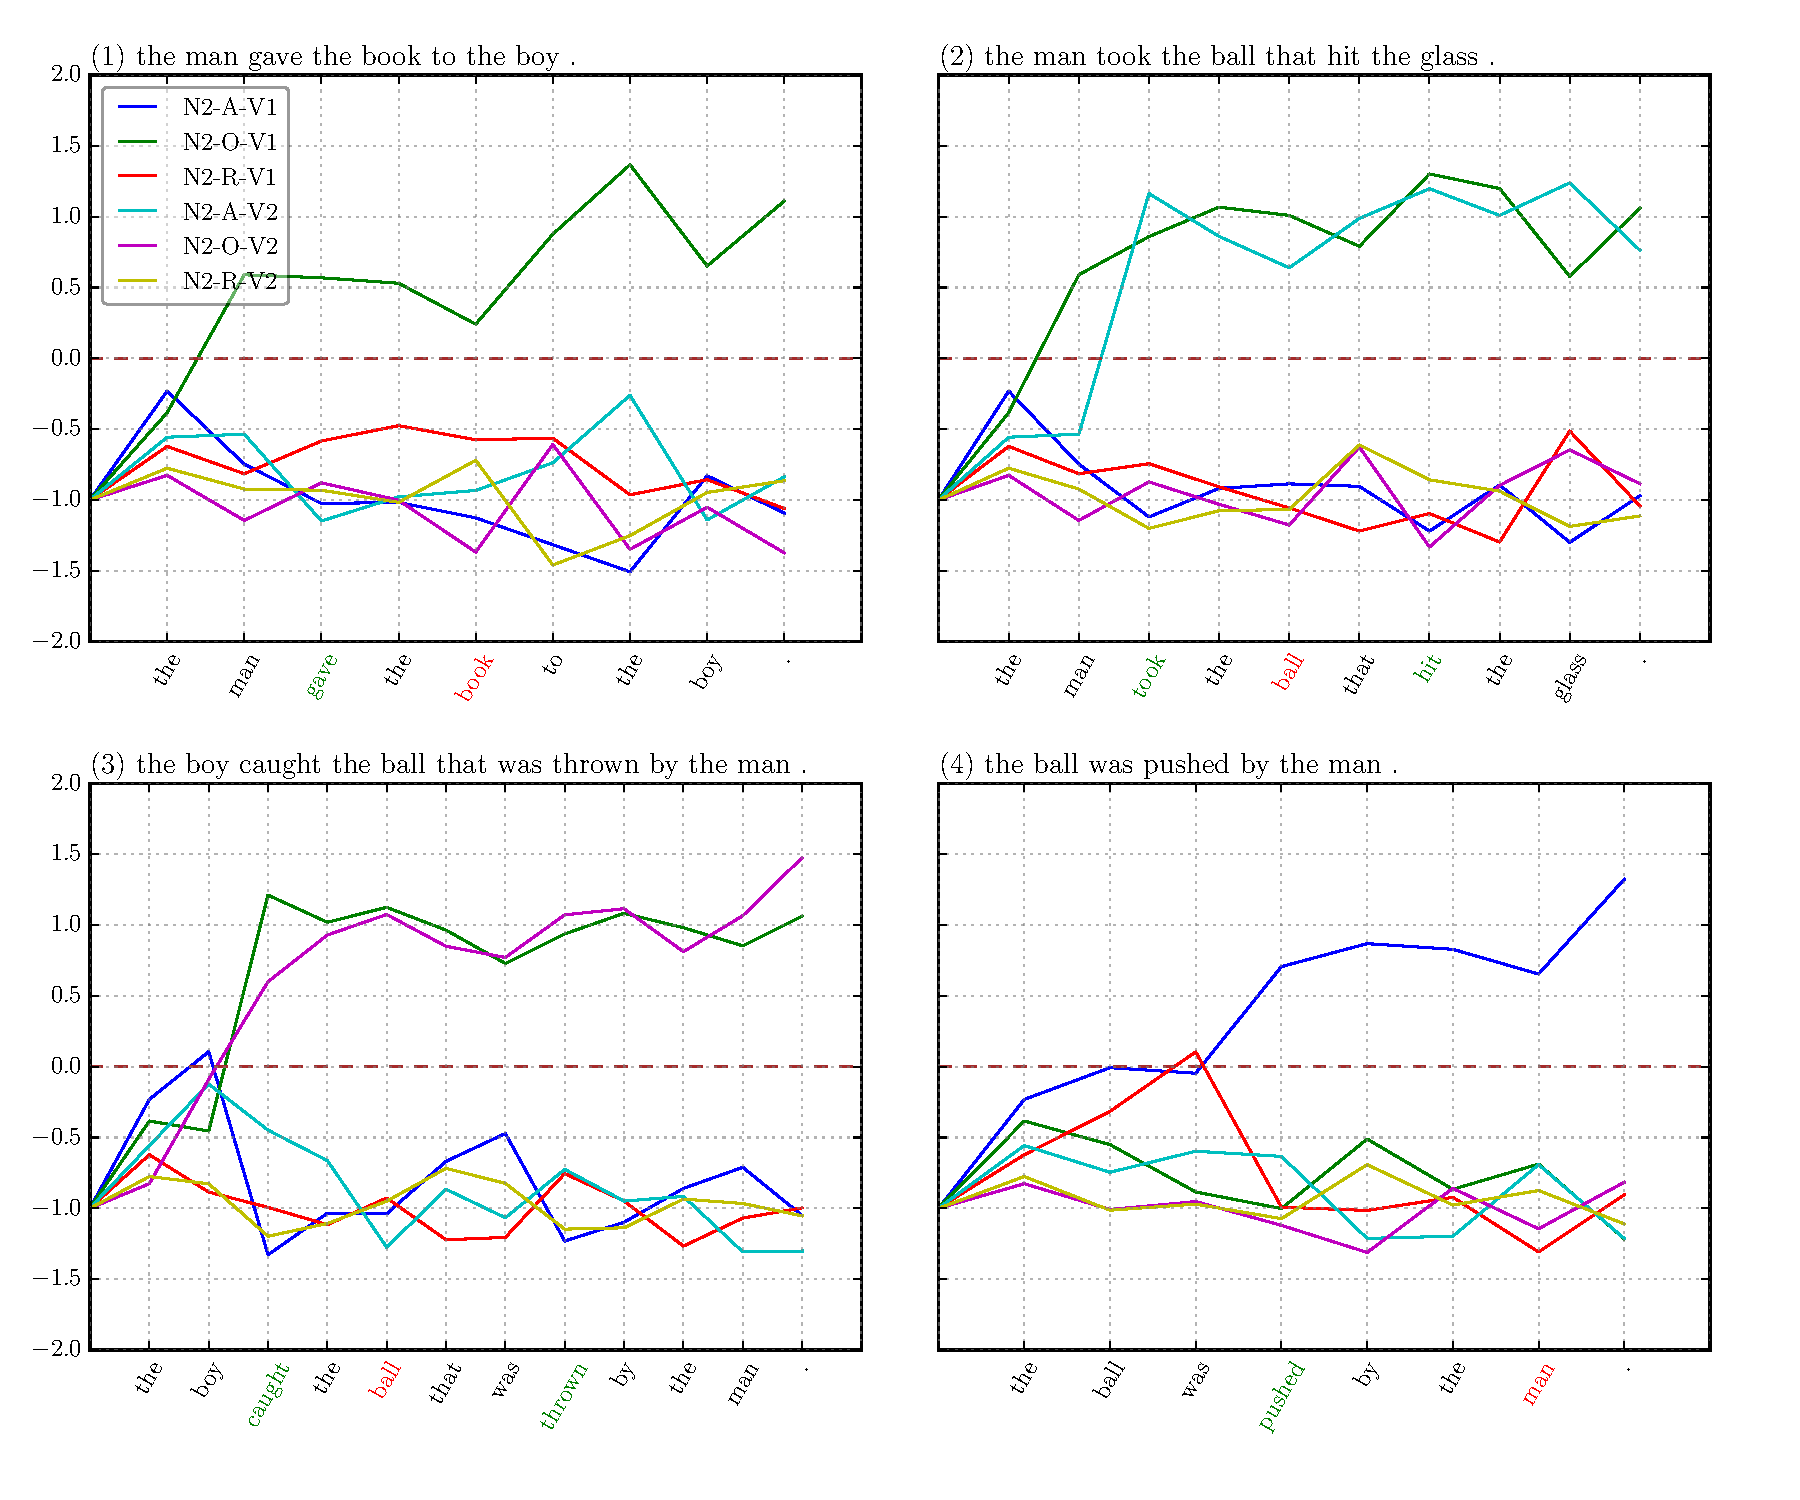
\includegraphics[width=1.0\linewidth]{act_analysis_1}
\caption[Readout activity of Word2Vec-$\theta$RARes model for a sentence with topologically modified coded meaning.]{\textbf{Readout activity of Word2Vec-$\theta$RARes model for a sentence with topologically modified coded meaning: } {\small Each coloured line shows the thematic role of Noun-2 (tick marked in red) with respect to Verb-1 and Verb-2 (ticks shown in green).}}
\label{fig:act_analysis_1}
\end{figure}

Each colored line in the graph (see fig. \ref{fig:act_analysis_1}) represents the possible thematic roles of the second noun (N2) which can have one of the three possible roles i.e. Agent (A), Object (O) or Recipient (R), with respect to either Verb-1 (V1) or Verb-2 (V2). N2 is marked in red and verbs are marked in green on the x-axis. In the figure, the role `N2-A-V1' can be interpreted as the second noun (N2) is the agent of the first verb (V1). 

As all the four sentences start with `the', the activations at this word is same for all four sentences. With the introduction of the first noun (`man') in sentences \ref{activation:sent-1} and \ref{activation:sent-2}, the readout activations of role N2 as object of V1 (N2-O-V1) goes above the threshold 0. Thus the model predicts that the N2 could be the object of V1. In sentence \ref{activation:sent-3}, with the arrival of the first noun (`boy'), the competition between roles N2-A-V1, N2-A-V2, and N2-O-V2 can be seen, but only the role N2-A-V1 (agent of verb `caught') managed to cross the threshold. Whereas, in sentence \ref{activation:sent-4}, the activation of role N2-A-V1 is higher when the first noun (`ball') is encountered, but with the arrival of `was' the role of N2 is changed as recipient of V1 (`pushed').

In sentence \ref{activation:sent-1}, the activation of role N2-A-V1 is maintained, and no other role managed to cross the threshold with the arrival of V1 (`gave')
Whereas in sentence \ref{activation:sent-2}, with the advent of the V1 (`took') the activation for N2-A-V2 goes above threshold, indicating the presence of V2 (`hit') in the sentence even before the model has encountered the second verb. In sentence \ref{activation:sent-3} and \ref{activation:sent-4}, with the arrival of V1 (`caught' and `pushed' respectively) one can notice the re-analysis made by the model. In sentence \ref{activation:sent-3}, the activation of N2-A-V1 goes below the threshold and takes the new role as the object of both V1 (`caught') and V2 (`thrown'), i.e., N2-O-V1 and N2-O-V2. In sentence \ref{activation:sent-4}, the previously predicted role N2-R-V1 goes below the threshold with the arrival of V1 (`pushed').

Throughout the rest of sentence \ref{activation:sent-1}, the prediction N2-O-V1 is maintained with some minor ups and downs. Similarly, in sentence \ref{activation:sent-2}, the predictions of N2 alternates between roles N2-O-V1 and N2-A-V2 but the activation of both the roles remains above the threshold. In sentence \ref{activation:sent-3} the model sees both N2-O-V1 and N2-O-V2 as the preferred predictions, both being almost with similar activations and only alternating slightly. In sentence \ref{activation:sent-4}, the prediction of role N2-A-V1 do not change again throughout the sentence ever since the arrival of V1 (`pushed').

It can be seen that, at the end of the sentences, the model predicted the meaning of all the four sentences correctly. Also, notice the early prediction of correct roles even before the sentence is completed. The distributed representation of words learned from the nearby words and possibly encapsulating the information about them can be credited for such behavior.

\subsection{Output activity for sentences without topologically modified coded meaning} 

Figure \ref{fig:act_analysis_2} shows the readout activations of the following two sentences taken from corpus-373. 

\begin{enumerate}[noitemsep,label=(\Alph*) ]
\item \textit{put}(X1) the \textit{cross}(X2) on my \textit{right}(X3) \label{activation:sent-a}
\item \textit{push}(X1) the \textit{triangle}(X2) to the \textit{left}(X3) then \textit{push}(X4) the \textit{cross}(X5) to the \textit{left}(X6) \label{activation:sent-b}
\end{enumerate}

\begin{figure}[hbtp]
\centering
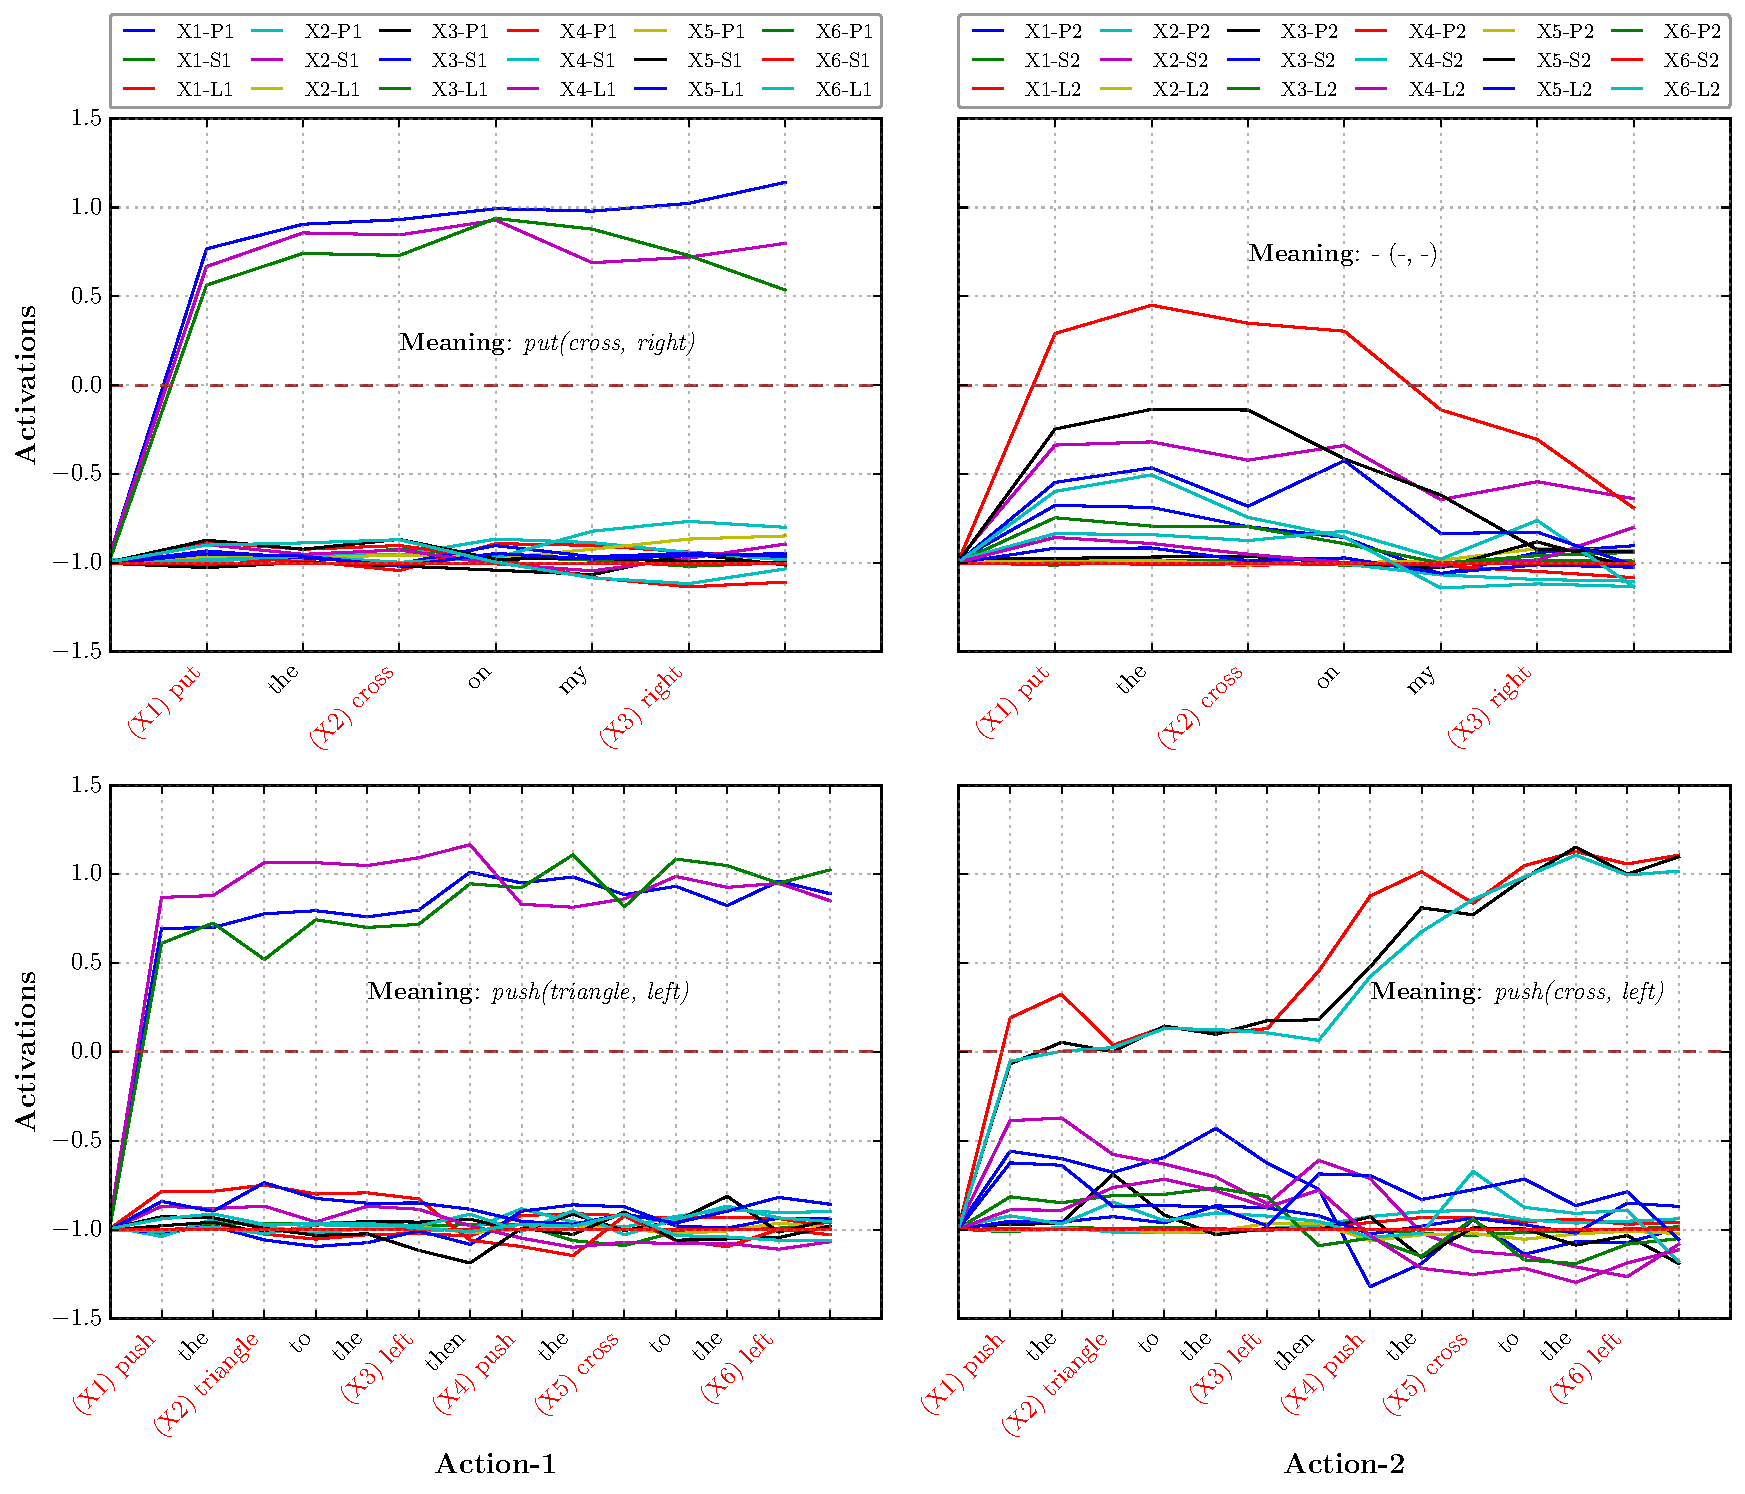
\includegraphics[width=1.0\linewidth]{act_analysis_2}
\caption[Readout activity of Word2Vec-$\theta$RARes model for a simple and complex sentence from corpus-373.]{\textbf{Readout activity of Word2Vec-$\theta$RARes model for a simple and complex sentence from corpus-373: }{\small First and second row shows the readout activation for a simple and complex sentence respectively. Each column in the figure shows the activation of the corresponding sentence with respect to an action.} }
\label{fig:act_analysis_2}
\end{figure}

Note that the sentence \ref{activation:sent-a} is a simple instruction to perform only one action and contains three semantic words (X1-X3). Whereas sentence \ref{activation:sent-b}, is a complex instruction to perform two actions and contains six semantic words (X1-X6). Each semantic word in the sentences can have a role with respect to a maximum of two actions (see corpus-373 in section \ref{corpora}). A role X1-P1, for example, is interpreted as the first semantic word (X1)  is the predicate of action-1. The roles predicate, subject and location are represented by `P', `S' and `L' respectively.

The first row of Figure \ref{fig:act_analysis_2} shows the readout activity of the model for sentence \ref{activation:sent-a} with respect to action-1 (left) and action-2 (right). One can see that for action-1, the model correctly predicts the meaning \textit{put(cross, right)}, whereas for the action-2, at the end of sentence all the neural activations go below the threshold 0. Thus, this indicates the presence of only action-1 in the sentence  \ref{activation:sent-a}. Also, for the action-2, notice the online re-analysis behavior of the model where the activation of role (X1-L2) goes above the threshold 0 at the beginning of the sentence but later drops below the threshold at the end of the sentence.

The second row of Figure \ref{fig:act_analysis_2} illustrates the readout activity of sentence \ref{activation:sent-b} for each action. The model correctly predicts the thematic roles of constituent semantic words (X1 to X6) for both the actions. For the action-1, the model makes early predictions of roles i.e. \textit{push (triangle, left)}, whereas, for action-2, the activation of correct roles are reinforced when the model encounters the second predicate (X4 = `push') in the sentence. Thus the model predicts the meaning of sentence for the second action as \textit{push (cross, left)}.

\section{Comparative Analysis of Sentences Meaning}

In the previous section, we saw the online re-analysis of sentences with and without the topologically modified coded meanings by the Word2Vec-$\theta$RARes model. So far, we have also seen the performance of Word2Vec-$\theta$RARes model in numbers. In this section, we will analyze for what type of sentences the Word2Vec-$\theta$RARes model correctly predicted the meanings, but the $\theta$RARes model failed. Also, we will see the kind of sentences for which the Word2Vec-$\theta$RARes model failed to predict the meaning correctly. This analysis was done on the results obtained in Experiment-6 using corpus-373.

While analyzing the sentences whose meanings were correctly predicted by all ten instances of the Word2Vec-$\theta$RARes model and incorrectly predicted by the $\theta$RARes model, a significant number of patterns were identified. Almost $85 \%$ of the sentences whose meaning were wrongly predicted by all the instances of $\theta$RARes model were either two action commands or redundant commands (see fig. \ref{fig:meaning_realtions}). For example, ``push the circle in the middle and put it in the right" and ``push the circle to the middle and then put it on the right".

Table \ref{tab:color_error} reports the example sentences whose meanings are correctly predicted by all the instances of Word2Vec-$\theta$RARes model and incorrectly predicted by at-least one instance of the $\theta$RARes model. The sentences in the table include only some examples to convey the findings. The Word2Vec-$\theta$RARes model correctly predicted the meaning of the sentences 
\begin{enumerate*}[(1)]

\item where the color of the objects to be moved is specified (sentences 1-5,11). In other words, the sentences where the adjectives, like \textit{`red'} or \textit{`blue'} are used with the semantic words

\item where the anaphoric reference word \textit{`it'} (sentences 6-8), pointing to a semantic word within the discourse of sentence is used

\item where an action to be repeated is specified using the anaphoric words `twice' or `two times' (sentences 9-12)

\item where a reference location is given with respect to the person instructing the robot (sentences 6, 13-14).
\end{enumerate*}
Whereas at least one instance of $\theta$RARes model incorrectly predicts the meaning of such sentences. 

% Please add the following required packages to your document preamble:
\begin{table}[hbtp]
\centering
\caption{Example sentences correctly predicted by all 10 instances of Word2Vec-$\theta$RARes model and mispredicted atleast once by  $\theta$RARes model. }
\label{tab:color_error}
\resizebox{\textwidth}{!}{%
\begin{tabular}{|c|l|l|l|}
\hline
\multicolumn{1}{|c}{\multirow{2}{*}{\textbf{S.No}}} & \multicolumn{1}{|c|}{\multirow{2}{*}{\textbf{Sentences}}} & \multicolumn{2}{c|}{\textbf{\begin{tabular}[c]{@{}c@{}}Actual  Meaning\\ Predicate(Object,Location)\end{tabular}}} \\ \cline{3-4} 
\multicolumn{1}{|c}{} & \multicolumn{1}{|c|}{} & \multicolumn{1}{c|}{\textit{\textbf{Action-1}}}& \multicolumn{1}{c|}{\textit{\textbf{Action-2}}}         \\ \hline

1&point the red cross and point the circle                           & point(cross, -)         & point(circle, -)     \\ \hline
2&put the red cross to the left and hit the blue circle              & put(cross, left)        & hit(circle, -)     \\ \hline
3&grasp the red cross and then point the circle                      & grasp(cross, - )        & point(circle, -)     \\ \hline
4&after putting the red cross to the left please hit the blue circle & putting(cross, left)    & hit(circle, -)     \\ \hline
5&please grasp the red cross                                           & grasp(cross, -)         &    -                \\ \hline
6&before grasping the triangle on my left point at it.     & point (triangle, -)  & grasping(triangle, -)   \\ \hline
7&before grasping the triangle point at it.                & point (triangle, -)  & grasping(triangle, -)   \\ \hline
8&before hitting the triangle point at it.                 & point (triangle, -)  & hitting (triangle, -)   \\ \hline
9&grasp circle two times                                     & grasp(circle, -)         & grasp(circle, -)          \\ \hline
10&point cross two times                                     & point(cross, -)         & point(cross, -)         \\ \hline
11&hit twice the blue circle                                 & hit(circle, -)         & hit(circle, -)         \\ \hline
12&grasp the circle twice                                     & grasp(circle, -)         & grasp(circle, -)           \\ \hline
13&point the circle on my left                              & point (circle, -)    & -                        \\ \hline
14&push the cross on my left and then grasp the circle      & push (cross, left)   & grasp (circle, -)     \\ \hline

\end{tabular}%
}
\end{table} 

So far, we have seen the upside of Word2Vec-$\theta$RARes model over $\theta$RARes model, but there are cases where Word2Vec-$\theta$RARes model fails as well. As reported in Table \ref{tab:common_error}, it was observed that in most of the cases, the meaning of the sentences with complex structures where the first action to be performed is specified after the second action using the phrase `after having' are predicted wrongly by the model (sentences 2-4). Also, the Word2Vec-$\theta$RARes model fails to predict the meaning of grammatically incorrect sentences in most of the cases (sentence 1). It was also noticed that the use of word contractions e.g. `youve', `weve' etc. in the sentences (sentences 5, 6) also leads to an error in meaning prediction by Word2Vec-$\theta$RARes model.

\begin{table}[h]
\centering
\caption{Example sentences for which the Word2Vec-$\theta$RARes model failed to predict the meaning correctly.}
\label{tab:common_error}
\resizebox{\textwidth}{!}{%
\begin{tabular}{|c|l|l|l|}
\hline
\multicolumn{1}{|c}{\multirow{2}{*}{\textbf{Sentences}}} & \multicolumn{1}{|c|}{\multirow{2}{*}{\textbf{Sentences}}} & \multicolumn{2}{c|}{\textbf{\begin{tabular}[c]{@{}c@{}}Actual  Meaning\\ Predicate(Object,Location)\end{tabular}}} \\ \cline{3-4} 
\multicolumn{1}{|c}{} & \multicolumn{1}{|c|}{} & \multicolumn{1}{c|}{\textit{\textbf{Action-1}}} & \multicolumn{1}{c|}{\textit{\textbf{Action-2}}} \\ \hline

1&in left push the triangle and the cross                  & push(triangle, left )   & push(cross, left)  \\ \hline
2&grasp the circle but before put the cross on the left    & put(cross, left )        & grasp(circle, -)    \\ \hline
3&touch the cross after having touch the triangle          & touch(triangle, -)        & touch(cross, -)     \\ \hline
4&put the triangle to the left after having touched it     & touched (triangle, -)     & put(triangle, left)   \\ \hline
5&touch the circle after youve pointed the triangle        & pointed(triangle, -)      & touch(circle, -)    \\ \hline
6&put the cross over to the left and then once youve & & \\ &done that grasp the circle   & put(cross, left ) & grasp(circle, -) \\ \hline

\end{tabular}
}
\end{table}
\cleardoublepage

\chapter{Conclusion And Future Work}\label{conclusion}

Previously, we saw the $\theta$RARes model which processes the sentences transformed to grammatical form and used the localist word representations to solve the TRA task \cite{xavier:2013:RT}. We have also seen the proposed neural-inspired language models (Word2Vec-$\theta$RARes and Word2Vec-ESN classifier) and the experiments performed using them. In this chapter, we finally conclude this research, first by summarizing the findings from the outcome of the experiments performed, then the possible future work identified during the development of this study.

\section{Conclusion}

This thesis started with the goal to test the hypothesis that distributed word representation in combination with a recurrent neural network could be used to achieve better performance on the TRA task. Thus, to test this hypothesis, Word2Vec-$\theta$RARes language model and Word2Vec-ESN classifier were proposed. Several experiments were performed using the proposed Word2Vec-$\theta$RARes model and the Word2Vec-ESN classifier. The outcomes of the experiments have led to the conclusion that follows.

\subsection{Generalization: Performance on unseen sentences}

One basic conclusion from this research is that the proposed Word2Vec-$\theta$RARes model using distributed word embeddings performs better than the $\theta$RARes model which processes the sentences transformed in the grammatical form using localist word vectors.

\paragraph{Performance on a limited number of sentences:} It was shown in Experiment-1, that the Word2Vec-$\theta$RARes model learned the sentences thoroughly when trained on limited sentences but failed to generalize on unseen sentences. Whereas, the  $\theta$RARes model was able to generalize better on the small corpus because of the generalization imposed in the data by replacing the semantic words with `SW' token while pre-processing. This leads us to a conclusion that $\theta$RARes model performs better on small corpus whereas Word2Vec-$\theta$RARes fails to do so. 

\paragraph{Performance on corpus-462 and corpus-90582:} Recall that the extended corpus-462 and corpus-90582 contain the sentences with the verb inflections (i.e. -ed, -ing, -s). For the same corpora, the $\theta$RARes model process the sentences transformed in the grammatical form using the localist word vectors. Thus, the input layer contains a unit for each closed class words, a unit to encode semantic word (`SW' token) and additional units to encode the verb inflections \cite{xavier:2013:RT}. Whereas, for the Word2Vec-$\theta$RARes model, the verbs with inflections in the corpora were replaced with the corresponding verb conjugations while preprocessing. The Word2Vec-$\theta$RARes model uses the topologically modified coded meaning for experiments with corpus-462 and corpus-90582. Use of verb inflections as an input to the $\theta$RARes model and topologically modified coded meaning with Word2Vec-$\theta$RARes model do not suffice the requirement of an end-to-end system. Both the $\theta$RARes and Word2Vec-$\theta$RARes model have to depend on a parser to extract the verb inflections and verbs respectively in a sentence. Thus the performance of the model becomes dependent on the accuracy of the parser. Assuming that the parser is 100 $\%$ accurate, the Word2Vec-$\theta$RARes model generalized on both the corpora but performed much better in the SCL mode as compared to that of the SFL mode, whereas it is vice-versa in $\theta$RARes model. Additionally, the Word2Vec-$\theta$RARes model outperforms the $\theta$RARes model in the SCL mode. The word embeddings learned from the nearby words and the capability of ESN to model the long-dependencies in the sentences can be credited for such behavior. In the SFL mode, the performance of both the Word2Vec-$\theta$RARes and $\theta$RARes model remained almost equivalent. So, it can be concluded that when both the models are dependent on a parser, the Word2Vec-$\theta$RARes model performs better than $\theta$RARes model.

The Word2Vec-ESN classifier also generalizes with high classification scores, when the raw sentences are processed using distributed words embeddings. When the sentences transformed in grammatical form and encoded using localist vector representation are used for processing, the classifier did not generalize well as shown by the low classification scores. Overall the results indicate that the distributed word embeddings improve the performance of the Word2Vec-ESN classifier over localist word vectors.

\paragraph{Performance on coprus-373:} As corpus-373 does not contain verb inflections, the $\theta$RARes model processes the sentences without using the input units for verb inflections. Also, the Word2Vec-$\theta$RARes model does not use topologically modified coding. This makes both the models independent of the parser and thus the performance of both the models can be compared. As shown in Experiment-6, the Word2Vec-$\theta$RARes model outperforms the $\theta$RARes model. Hence, it can be concluded that the semantic and syntactic information captured in distributed word vectors helps the Word2Vec-$\theta$RARes model to enhance the performance on the TRA task.

\subsection{Effect of reservoir and corpus sizes}

It was also shown that the generalization ability of the Word2Vec-$\theta$RARes model on the TRA task also increases with increase in reservoir and corpus size but asymptotes at a point. With the increase in both the reservoir and corpus size, the Word2Vec-$\theta$RARes model generalized better in SCL mode than in SFL mode. However, the generalization ability in both the learning modes becomes stable if the corpus and reservoir size is further increased from the asymptotic point. Overall, the conclusion which can be drawn from this is that with large corpus and reservoir size the Word2Vec-$\theta$RARes model generalizes better.

The Word2Vec-ESN classifier, on the other hand, achieved the high classification score even with the smaller reservoir of 250 neurons. The performance of the model does not deviate much with the further increase in reservoir size. Thus the model can be used with small reservoir size which makes it computationally cheaper for the TRA task.

\subsection{Structure of corpus}

The results of Experiments 2 and 3, shows that the Word2Vec-$\theta$RARes model generalizes well in both the SCL and SFL mode when the inherent grammatical structure is present in the sentences but fails to generalize when the word order in the sentences is scrambled. Thus we can conclude that the Word2Vec-$\theta$RARes model is not generalizing on any inconsistent regularity in the corpus but, instead, exploiting the inherent grammatical structure of the sentences to learn and generalize.

The Word2Vec-ESN classifier, on the other hand, generalized with high classification scores with the scrambled corpus in configuration-1 (with distributed word embeddings). However, this behavior is not surprising at all. The answer to this behavior lies in the way the Word2Vec-ESN classifier is trained. Recall that unlike Word2Vec-$\theta$RARes model, the Word2Vec-ESN classifier is trained to classify an argument-predicate pair to a role. So the model learns the mapping between the argument-predicate pairs and the corresponding roles. So even if the word order is changed, the model utilizes the semantic and syntactic information and also the information captured about context words in word embeddings, to classify the argument-predicate pairs correctly. Hence, it can be said that the Word2Vec-ESN classifier can perform better with distributed embeddings in the cases where sentences are not completely grammatically correct.

In configuration-2 (with localist word vectors), the Word2Vec-ESN classifier failed to generalize on the scrambled corpus. The reason is the transformation of sentences to grammatical form. The use of same `SW' token for all semantic words and encoding the words in localist fashion confuses the model to assign the appropriate thematic role to the input argument-predicate pair thus leading to failure in generalization. 

\subsection{Robustness of the model}

Recall that the Word2Vec-$\theta$RARes processes the corpus-373 without using the topologically modified coded meaning. However, it was shown in Experiment-6, that the model gracefully generalized well on corpus-373, using the same model parameters learned from corpus-462 with the topologically modified coded meaning. Thus, it can also be concluded that the model parameters are robust enough to generalize on new corpora for the TRA task. However, there is a possibility to optimize the performance further on corpus-373 with Word2Vec-$\theta$RARes model by optimizing the ESN parameters on this corpus.

\subsection{Dimension of word vectors}

Mikolov et al. \cite{w2v:mikolov_2013_efficient,w2v:mikolov_2013_distributed} showed that the higher dimensional word embeddings performed better on the word analogy task as compared to word vectors with lower dimensions. We have seen in the result of Experiment-7, that the dimensions of distributed word vectors,  do not affect the performance of Word2Vec-$\theta$RARes model significantly on the TRA task. However, the larger word vector dimensions increased the computation cost, but the performance gain was negligible. So, following Occam's razor principle which states that ``It is vain to do with more what can be done with fewer" \cite{razor:franklin_2002}, it can be concluded that the smaller word vectors should be preferred over larger ones with the Word2Vec-$\theta$RARes model for the TRA task.

\subsection{Online re-analysis of sentence meanings}

In addition to the generalization on unseen sentences, it was also shown that the proposed Word2Vec-$\theta$RARes model also do the re-analysis of the sentence meanings upon arrival of each word. The read-out activity of the model changes each time a new word is input to the model. The read-out activations at any time step can be interpreted as an estimated prediction of the sentence meaning for the input given so far \cite{xavier:2013:RT}. This behavior is not something new. The online re-analysis of sentence meanings was also observed with the $\theta$RARes model. However, the use of word embeddings learned from the context words and possibly encapsulating the information about neighboring words enables the Word2Vec-$\theta$RARes model to make a very early prediction of the sentences meaning. This behavior seems to be natural in humans when a sentence is being heard. A person listening to a sentence starts predicting the meaning of a sentence as soon as he/she listens to the first few words by making assumptions, gained from previous experiences. This advantage of early prediction can be useful for Human-Robot Interaction (HRI). A robot can start making actions, using the output activations even before the completion of the sentence \cite{tra:xavier_hri}.

The Word2Vec-ESN classifier considers the TRA task as a classification problem. The training objective of the classifier is to classify the argument-predicate pairs to the thematic roles. Thus, unlike the Word2Vec-$\theta$RARes model, the Word2Vec-ESN classifier was not teacher forced with the meaning of the whole sentence during training but, instead with the thematic role of the current argument-predicate pair. Thus it is not possible for the Word2Vec-ESN classifier to do the online re-analysis of sentence meaning.

\subsection{Word2Vec-$\theta$RARes vs Word2Vec-ESN classifier}

We have seen that the Word2Vec-$\theta$RARes model and Word2Vec-ESN classifier process the sentences differently and are evaluated using different metrics. As the performance of both the models is evaluated with different metrics, it would not be fair to claim which one of them performs better. However, it can be argued that both the models perform better when distributed word embeddings are used over localist word vectors. For the TRA task, both models could be employed. Each model has its own advantages and limitations which are stated below:

\paragraph{Input coding:} The Word2Vec-$\theta$RARes model process a sentence word by word. Thus the model takes a word as an input at each time step. Whereas, the Word2Vec-ESN classifier takes an argument-predicate pair as input. To identify the predicates (verbs) in a sentence, the Word2Vec-ESN classifier has to depend on a syntactic parser. Hence the performance of the Word2Vec-ESN classifier also depends on the accuracy of the parser. This is one of the limitations of Word2Vec-ESN classifier.

\paragraph{Output coding:} The output units of the Word2Vec-$\theta$RARes model encode the thematic roles of semantic words. Thus, in order to encode the thematic roles for all possible semantic words in any sentence, the maximum number of semantic words a sentence can have in the corpus should be known in prior. Also, the number of output units increases with the number of semantic words and the thematic roles a semantic word can have. The increase in the number of output units also increases the number of learnable reservoir-to-outputs weights ($W^{out}$) and hence the computational cost also increases. Unlike the Word2Vec-$\theta$RARes model, the number of output units in the Word2Vec-ESN classifier remains independent of the number of semantic words a sentence can have. The number of output units is always equal to the number of thematic roles which a word can have. Therefore, the limited number of output units makes the Word2Vec-ESN classifier computationally cheap. 

\paragraph{Reservoir size:} The Word2Vec-$\theta$RARes model requires a bigger reservoir for generalization, whereas the Word2Vec-ESN classifier generalizes with a small reservoir size. Generalization with the small reservoir size also makes the Word2Vec-ESN classifier computationally cheap and hence a preferable choice over Word2Vec-$\theta$RARes model.

\paragraph{Online re-analysis of sentence meaning:} As discussed earlier, the Word2Vec-$\theta$RARes have the capability to make online re-analysis of sentence meaning across time. In some cases, the model also predicts the meaning of sentences even before the completion of the sentence. This advantage of online re-analysis and early prediction is not possible with the Word2Vec-ESN classifier.

\section{Future Work}

In this research, the proposed Word2Vec-ESN classifier makes an assumption that the syntactic parser used to identify verbs is $100 \%$ accurate. It would be interesting to explore the behavior of the Word2Vec-ESN classifier with the most accurate syntactic parser like Stanford parser \cite{parser:stanford}, Charniak parser \cite{charniak_parser:2000}, Bikel parser \cite{parser:bikel:2004} or Berkley parser \cite{parser:berkley:2006}.

As described earlier, the Word2Vec model implementation has been modified to update the vocabulary of an already trained model. The new words can be added to the vocabulary and distributed embeddings can be learned for them. Thus the modified implementation of the Word2Vec model can be extended to make the proposed models, ever-learning systems for the TRA task. However, updating the Word2Vec model with every sentence was also attempted during this research work, but because the computational time was really high and the performance gain was negligible, it was left unexplored for the future work. It would be interesting to explore how the model can be updated in an online manner with the minimal computational time so that it can be feasibly implemented on the robotics platform. 

For this work, the combination of the Word2Vec model and ESN was used. The ESN has an advantage of modeling sequential data. Thus the sequential and temporal aspect of a sentence is taken into account in this study for thematic role assignment. However, the dependencies between the thematic roles of words in the sentences were not taken into consideration for learning. To model the conditional probability distribution of the thematic roles of words, Conditional Random Fields (CRF); a log-linear model; could be used \cite{crf:intro:sutton}. CRFs have been one of the most successful approaches used earlier as well for classification and sequential data labeling tasks \cite{end-to-end, esn:esn_crf}. Thus the Word2Vec-ESN classifier, proposed in this study, could be used with an additional CRF unit to model the temporal dependencies between the input sentences conditional on the corresponding thematic roles. Doing so allows the resulting model to capture the concealed temporal dynamics present in the sentences \cite{esn:esn_crf}. It is also important to know that addition of CRF with Word2Vec-$\theta$RARes model does not make any sense because, unlike Word2Vec-ESN classifier, the model takes the meaning of the whole sentence as teacher output to learn thematic roles. 

Distributed word vectors obtained by training the Word2Vec model on one language corpus (e.g., English) can also be translated to get the most similar word in any other target language (e.g., French). This translation is achieved by linearly projecting (rotation and scaling) the word vectors of source language on the target language \cite{w2v:language_similarities}. Thus the Word2Vec-$\theta$RARes language model can also be investigated further for multiple language acquisition \cite{hinaut_multiple_lang}. 
\cleardoublepage

%%%%%%%%%%%%%%%%%%%%%%%%%%%%
% Appendices:
% these are optional! For most Bachelor-theses and some Master-thesis none of them is needed. 
% Just comment them if not needed.
\appendix
\fancyhead[LO,RE]{}                      % Define the header style for the appendixpages

\fancyhead[LE,RO]{\it Appendix A. Complete Simulation Results}%Adapt letter!
  \chapter{Complete Simulation Results}\label{app:completeResults}


%NOTE: 08/09/2016 results are copied after the simulation and are final, no need to change.
\begin{table}
\centering
\begin{threeparttable}
\caption{Effect of reservoir size on Word2Vec-$\theta$RARes model in different learning modes.}
\label{tab:corpus-size}
\rowcolors{2}{white}{gray!25}
\begin{tabularx}{\textwidth}{llYYYY}
  \toprule
  \hiderowcolors   
  &  & \multicolumn{4}{c}{Word2Vec-$\theta$RARes Model} \\
  \cmidrule(lr){3-6}   
  
Reservoir size  &  & \multicolumn{2}{c}{SCL mode} & \multicolumn{2}{c}{SFL mode} \\
  \cmidrule(lr){3-4} \cmidrule(lr){5-6}   
    
	   			& 			& ME 	& SE 		& ME 	 & SE 			\\
  \midrule
  \showrowcolors
  \textbf{90} 	& mean 		& 38.30 & 92.52  	& 46.41  & 98.09	 	\\
   			    & std 		& 1.53  & 1.67 		& 1.02   & 1.29 		\\
   			    		
  \textbf{291} 	& mean  	& 17.68 & 60.26 	& 22.00   & 69.13 		\\
				& std  		& 0.80 & 1.74 		& 0.97   & 3.03  		\\
  			   			
  \textbf{493} 	& mean 		& 11.63 & 40.34 	& 13.60   & 45.61 		\\
  				& std 		& 0.65 & 2.58 		& 0.64   & 2.14 		\\
  				 		
  \textbf{695}	& mean  	& 9.76 & 32.56 		& 10.64   & 34.83 		\\
  			  	& std 		& 0.61 & 1.56		& 0.58   & 1.42  		\\
					
  \textbf{896}	& mean  	& 8.39 & 25.56 		& 9.79   & 28.70 		\\
  			  	& std 		& 0.32 & 0.73		& 0.50   & 0.60  		\\
					
  \textbf{1098}	& mean  	& 7.98 & 22.17 		& 9.41   & 26.09 		\\
  			  	& std 		& 0.56 & 1.45		& 0.26   & 1.14  		\\
  			  		
  \textbf{1776}	& mean  	& 7.57 & 19.65 		& 9.79   & 24.70 		\\
  			  	& std 		& 0.39 & 0.84		& 0.43   & 0.90  		\\
  			  		
  \textbf{2882}	& mean  	& 6.99 & 18.04 		& 10.85   & 26.22 		\\
  			  	& std 		& 0.55 & 1.00		& 0.90   & 1.61  		\\
  			  		
  \textbf{3988}	& mean  	& 7.20 & 17.74 		& 11.02   & 26.17 		\\
  			  	& std 		& 0.48 & 0.45		& 0.50   & 1.63  		\\
  
  \textbf{5094}	& mean  	& 7.07 & 17.83 		& 11.06   & 25.87 		\\
  			  	& std 		& 0.53 & 1.54		& 1.08   & 1.34  		\\
  \bottomrule
\end{tabularx}
\begin{tablenotes}
\small
\item 
Meaning (ME) and Sentence error (SE) in different learning modes with Word2Vec-$\theta$RARes model. The errors are given in percentage and averaged over several model instances. The reservoir size is shown in first column. SCL: Sentence Continuous Learning; SFL: Sentence Final Learning; std: standard deviations. Simulations were performed with 5 model instances. Model was tested using 10-fold cross-validation approach.
\end{tablenotes}
\end{threeparttable}
\end{table}






%NOTE: 08/09/2016 results are copied after the simulation and are final, no need to change.
\begin{table}
\centering
\begin{threeparttable}
\caption{Effect of reservoir size on Word2Vec-ESN classifier in two different configurations.}
\label{tab:corpus-size}
\rowcolors{2}{white}{gray!25}
\begin{tabularx}{\textwidth}{llYYYYYY}
  \toprule
  \hiderowcolors   
  &  & \multicolumn{6}{c}{Word2Vec-ESN Classifier} \\
  \cmidrule(lr){3-8}   
  
Reservoir size  &  & \multicolumn{3}{c}{Configuration-1} & \multicolumn{3}{c}{Configuration-2} \\
  \cmidrule(lr){3-5} \cmidrule(lr){6-8}   
    
	   			& 			& Pr 	& Re 		& F1		& Pr 	 & Re 		& F1\\
  \midrule
  \showrowcolors
  \textbf{50} 	& mean 		& 83.09 & 52.59		& 61.12  	& 61.78  & 46.31	& 51.23 	\\
   			    & std 		& 4.57  & 7.76 		& 8.10		& 1.00   & 4.05 	& 3.11	\\
   			    		
  \textbf{100} 	& mean  	& 92.47 & 84.67		&88.05 		& 61.90  & 61.26 	& 60.72	\\
				& std  		& 1.14 	& 1.87		&1.37 		& 0.19   & 1.22  	& 0.58	\\
  			   			
  \textbf{250} 	& mean 		& 96.35 & 91.35 	&93.58		& 61.84  & 65.24 	& 62.51	\\
  				& std 		& 0.39 	& 0.25 		&0.18		& 0.10   & 0.84 	& 0.36	\\
  				 		
  \textbf{400}	& mean  	& 97.04 & 91.62		&94.03 		& 61.87  & 65.54 	& 62.67	\\
  			  	& std 		& 0.34 	& 0.24		&0.19		& 0.05   & 1.43  	& 0.62	\\
					
  \textbf{600}	& mean  	& 96.88 & 91.77		&94.05 		& 62.00  & 66.98 	& 63.21	\\
  			  	& std 		& 0.13 	& 0.13		&0.10		& 0.08   & 0.54  	& 0.24	\\
					
  \textbf{800}	& mean  	& 96.69 & 91.83		&94.00 		& 61.94  & 67.10 	& 63.30	\\
  			  	& std 		& 0.19 	& 0.07		&0.10		& 0.04   & 0.51  	& 0.26	\\
  			  		
  \textbf{1050}	& mean  	& 96.73 & 91.80		&94.01 		& 62.03  & 67.77 	& 63.54	\\
  			  	& std 		& 0.13 	& 0.03		&0.07		& 0.03   & 0.29  	& 0.17	\\
  			  		
  \textbf{1600}	& mean  	& 96.57 & 91.70		&93.88 		& 61.92  & 68.37 	& 63.85	\\
  			  	& std 		& 0.17 	& 0.10		&0.13		& 0.02   & 0.57  	& 0.23	\\
  			  		
  \textbf{2250}	& mean  	& 96.29 & 91.52 	&93.62		& 61.82  & 68.33 	& 63.82	\\
  			  	& std 		& 0.13 	& 0.05		&0.09		& 0.07   & 0.83  	& 0.37	\\
  
  \textbf{3320}	& mean  	& 96.05 & 91.38 	&93.46		& 61.80  & 68.24 	& 63.83	\\
  			  	& std 		& 0.22 	& 0.19		&0.21		& 0.08   & 0.94  	& 0.39	\\
  			  	
  \textbf{3860}	& mean  	& 96.07 & 91.39 	&93.47		& 61.85  & 67.74 	& 63.57	\\
  			  	& std 		& 0.22 	& 0.11		&0.15		& 0.05   & 2.80  	& 1.19	\\
  			  	
  \textbf{4500}	& mean  	& 95.91 & 91.28 	&93.34		& 61.89  & 70.01 	& 64.42	\\
  			  	& std 		& 0.25 	& 0.03		&0.13		& 0.07   & 3.60  	& 1.51	\\
  \bottomrule
\end{tabularx}
\begin{tablenotes}
\small
\item 
Precision (Pr), Recall (Re) and F1-Score (F1) in different configuration of Word2Vec-ESN classifier. The scores are given in percentage and averaged over several model instances. Configuration-1: raw sentences are processed, and distributed vectors of the argument-predicate pairs are input to ESN. Configuration-2: Sentences transformed to grammatical form and localist word vectors are input to ESN. std: standard deviations. Simulations were performed with 5 model instances. Model was tested using 10-fold cross-validation approach.
\end{tablenotes}
\end{threeparttable}
\end{table}


%NOTE: 08/09/2016 results are copied after the simulation and are final, no need to change.
\begin{table}
\centering
\begin{threeparttable}
\caption{Effect of sub-corpora size on Word2Vec-$\theta$RARes model in different learning modes.}
\label{tab:corpus-size}
\rowcolors{2}{white}{gray!25}
\begin{tabularx}{\textwidth}{llYYYY}
  \toprule
  \hiderowcolors   
  &  & \multicolumn{4}{c}{Word2Vec-$\theta$RARes Model} \\
  \cmidrule(lr){3-6}   
  
sub-corpora size  &  & \multicolumn{2}{c}{SCL mode} & \multicolumn{2}{c}{SFL mode} \\
  \cmidrule(lr){3-4} \cmidrule(lr){5-6}   
    
	   					& 		& ME 	& SE 		& ME 	 & SE 			\\
  \midrule
  \showrowcolors
  \textbf{5 $\%$} 	& mean 		& 12.18 & 54.84  	& 11.96  & 54.15	 	\\
   			    	& std 		& 0.19  & 0.52 		& 0.35   & 1.28 		\\
   			    		
  \textbf{12 $\%$} 	& mean  	& 6.13 & 32.63 		& 6.89   & 34.92 		\\
  			   		& std  		& 0.03 & 0.46 		& 0.18   & 0.78  		\\
  			   			
  \textbf{25 $\%$} 	& mean 		& 3.74 & 21.48 		& 4.91   & 26.10 		\\
  				 	& std 		& 0.04 & 0.42 		& 0.12   & 0.78 		\\
  				 		
  \textbf{50 $\%$}	& mean  	& 2.96 & 17.25 		& 4.17   & 22.41 		\\
  			  		& std 		& 0.04 & 0.39		& 0.11   & 0.57  		\\
					
  \textbf{75 $\%$}	& mean  	& 2.72 & 15.98 		& 3.95   & 21.33 		\\
  			  		& std 		& 0.03 & 0.30		& 0.11   & 0.64  		\\
					
  \textbf{100 $\%$}	& mean  	& 2.60 & 15.40 		& 3.84   & 20.78 		\\
  			  		& std 		& 0.02 & 0.25		& 0.09   & 0.57  		\\
  \bottomrule
\end{tabularx}
\begin{tablenotes}
\small
\item 
Meaning (ME) and Sentence error (SE) in different learning modes with Word2Vec-$\theta$RARes model. The errors are given in percentage. The sub-corpora (first column) is randomly sampled from corpus-90582. SCL: Sentence Continuous Learning; SFL: Sentence Final Learning; std: standard deviations. Simulations were performed with 5 model instances each having a reservoir of 1000 neurons. Model was tested using 10-fold cross-validation approach.
\end{tablenotes}
\end{threeparttable}
\end{table}




%NOTE: 08/09/2016 results are copied after the simulation and are final, no need to change.
\begin{table}
\centering
\begin{threeparttable}
\caption{Effect of word vector dimensions on Word2Vec-$\theta$RARes model in different learning modes.}
\label{tab:word-vector-size}
\rowcolors{2}{white}{gray!25}
\begin{tabularx}{\textwidth}{llYYYYYY}
  \toprule
  \hiderowcolors   
  &  & \multicolumn{6}{c}{Word2Vec-$\theta$RARes Model} \\
  \cmidrule(lr){3-8}   
  
  &  & \multicolumn{3}{c}{SCL mode} & \multicolumn{3}{c}{SFL mode} \\
  \cmidrule(lr){3-5} \cmidrule(lr){6-8}   
    
	   				& 			& ME 	& SE  	&	Best		& ME 	 & SE 		& Best		\\
  \midrule
  \showrowcolors
  \textbf{20} 		& mean 		& 14.68 & 40.46 & 	25.74		& 17.25  & 44.93 	& 29.49	 	\\
   			    	& std 		& 0.58  & 1.58 	&	-			& 0.76   & 1.36	 	& -			\\
   			    		
  \textbf{30} 		& mean  	& 14.23 & 39.87 &	26.01		& 16.61  & 43.46 	& 26.27 	\\
  			   		& std  		& 0.53 	& 0.57 	&	-			& 0.67   & 0.70  	& - 		\\
  			   			
  \textbf{50} 		& mean 		& 14.29 & 40.29 &	25.73		& 17.34  & 43.99 	& 26.54		\\
  				 	& std 		& 0.34 	& 1.13 	&	-			& 0.36   & 1.38 	& -		\\
  				 		
  \textbf{100}		& mean  	& 14.68 & 40.46 &	24.93		& 17.66  & 44.96 	& 30.02		\\
  			  		& std 		& 0.58 	& 1.58	&	-			& 0.55   & 1.66  	& -			\\
					
  \textbf{200}		& mean  	& 15.00 & 41.31 &	27.88		& 17.96  & 44.66 	& 29.49		\\
  			  		& std 		& 0.73 	& 1.55	&	-			& 0.63   & 1.19  	& -			\\
					
  \textbf{300}		& mean  	& 16.17 & 42.39	& 	31.36		& 19.19  & 46.51 	& 32.71		\\
  			  		& std 		& 0.75 	& 1.46	&	-			& 0.64   & 1.34  	& -	\\
  \bottomrule
\end{tabularx}
\begin{tablenotes}
\small
\item 
Meaning (ME), Sentence Error (SE) and Best value  for different word vector dimensions in different learning modes with Word2Vec-$\theta$RARes model. The errors are given in percentage. SCL: Sentence Continuous Learning; SFL: Sentence Final Learning; std: standard deviations. Simulations were done using corpus-373, with 10 model instances each having a reservoir of 1000 neurons. Model was tested using LoO cross-validation approach.
\end{tablenotes}
\end{threeparttable}
\end{table}
\cleardoublepage

% ... add as much appendices as you need (one can also add source code, for example)

%\fancyhead[LE]{\it \leftmark}
%\chapter{}
\fancyhead[LE,RO]{\it Bibliography}       % A bibliography never have a letter or numbering!
    \bibliographystyle{plain}             % Style for presenting the literature
    \addcontentsline{toc}{chapter}{Bibliography}% Add to the TOC
    \bibliography{thesis,esn,word2vec}
\cleardoublepage

%%%%%%%%%%%%%%%%%%%%%%%%%%%%
% Formal page 1
\vspace{2cm}
\chapter*{Erkl\"arung der Urheberschaft}
\label{sec:urheber}
\fancyhead[LE]{\it Erkl\"arung der Urheberschaft}
Ich versichere an Eides statt, dass ich die \trtype{} im Studiengang \trcourseofstudies{} selbstst\"andig verfasst und keine anderen als die angegebenen Hilfsmittel -- insbesondere keine im Quellenverzeichnis nicht benannten Internet-Quellen -- benutzt habe. Alle Stellen, die w\"ortlich oder sinngem\"a{\ss} aus Ver\"offentlichungen entnommen wurden, sind als solche kenntlich gemacht. Ich versichere weiterhin, dass ich die Arbeit vorher nicht in einem anderen Pr\"ufungsverfahren eingereicht habe und die eingereichte schriftliche Fassung der auf dem elektronischen Speichermedium entspricht.

%Ich versichere an Eides statt, dass ich die vorliegende \trtype{} selbstst\"andig und ohne unerlaubte Hilfe Dritter angefertigt habe. Alle Stellen, die inhaltlich oder w\"ortlich aus anderen Ver\"offentlichungen stammen, sind kenntlich gemacht. Diese Arbeit lag in gleicher oder \"ahnlicher Weise noch keiner Pr\"ufungsbeh\"orde vor und wurde bisher noch nicht ver\"offentlicht.

\vspace{4cm}
\noindent Ort, Datum \hfill Unterschrift

%The backcover is always empty
\newpage
\thispagestyle{empty}
\hspace{1cm}
\newpage

%%%%%%%%%%%%%%%%%%%%%%%%%%%%
% Formal page 2
\vspace{2cm}
\chapter*{Erkl\"arung zur Ver\"offentlichung}
\label{sec:urheber}
\fancyhead[LE]{\it Erkl\"arung zur Ver\"offentlichung}
Ich erkl\"are mein Einverst\"andnis mit der Einstellung dieser \trtype{} in den Bestand der Bibliothek.

\vspace{4cm}
\noindent Ort, Datum \hfill Unterschrift

%The backcover is always empty
\newpage
\thispagestyle{empty}
\hspace{1cm}
\newpage

\end{document}
%EOF

